\chapter{Background} \label{chap:Background}
% Introduce this section - 1 paragraph
%This section focuses on the history of the \gls{mr} leading to a definition of \gls{ar}.
This section begins by exploring the history of human vision research, tracing its development to our current understanding of human perception and its integration with \gls{mr} hardware.
We then look at the research behind how depth perception and perception can be considered with \gls{mr} \glspl{hmd}.
Followed by a systematic literature review of \gls{ar} enabled \gls{X-ray Vision}.
The discussion then shifts to volume rendering, emphasizing human-centered research using \gls{dvr}, and concludes with an analysis of illustrative effects and their applications within \gls{dvr}.

%\section{Perception and How it Relates to Augmented Reality (AR) and Virtual Reality (VR)}

\section{Human Perception and Depth Perception}
\begin{figure}
    \centering
    \includegraphics[width=\textwidth]{Chapter2/Images/CuttingDepthGraph.png}
    \caption[This graph of depth cues and distance provides guidelines for depth perception in relation to the distance and key perception parameters.]{
    This graph of depth cues and distance provides guidelines for depth perception in relation to the distance and key perception parameters. Used with permission from Cutting and Vishton~\cite{Vishton1995}.
    }
    \label{fig:CuttingDepthGraph}
\end{figure}

% a very fast history of perception science
Understanding the mechanisms of how perception works has been a goal for humans long before computing or \gls{mr} devices.
Perception has been studied since Democritus conceived that sight was formed from small indivisible particles (460-371 BC). 
Since then, we have learned the anatomical structures of eyes and that sight is processed in the mind rather than the eye (1011 - 1021).
During the 18th century, we started to gain a more modern view of how people see light (based on the reflection of light off of other objects), and we began to learn about how we observe beauty, aesthetics, and apparent deceptions. 
Newton's particle theory in Optics (1704) proposed that light is composed of small particles that travel in straight lines. These particles change direction and speed when they hit a reflective surface, dispersing into different colors. 
This started a revolutionary shift in our perception of light. Later findings disproved the belief in pure white light despite Goethe's defense of Aristotle's theory (1810).
This understanding of vision enabled technologies like motion images (developed in 1932), leading to the first motion picture projector (the Phantoscope) in 1895. 

% psycho physics has some importance for your thesis
In 1889, Gustav Fechner~\cite{alma9911190913502466} coined psycho-physical, and we developed a metric for quantitatively determining changes in people's perception.
Their study involved seeing at what point a user could no longer determine if more or fewer dots were in a pair of images. 
All pairs of images had ten more or fewer dots than the other one. 
This study showed that the more dots placed on a page, the harder it is for someone to determine the difference, creating the foundation of psychophysics analytics~\cite{alma9911190913502466}. 
From this point, qualitative experiments on perception began to run, and it became possible to understand precisely how human perception functioned.
Leading to our current understanding of topics like depth perception.

\subsection{Depth Perception Fundamentals}
Throughout the late 19\textsuperscript{th} century and the 20\textsuperscript{th} century, psychologists began to study depth perception and came up with many factors to describe it.
Most of these findings believed that depth perception was created by utilizing accommodation, convergence, motion perspective, binocular disparities, height of the visual field, aerial perspective, occlusion, and the relative size and density of objects~\cite{Vishton1995}.
In 1995, Cutting and Vishton took over a century's worth of research and concluded that the human ability to determine what parameters of depth perception are required to be effective.
Notably, not all depth cues are equal, and many are situational.
\autoref{fig:CuttingDepthGraph} shows a breakdown of how these depth cues can be contrasted based on how far away they are from each other. The obvious difference between the depth of two objects is shown using the virtual axis, while the horizontal axis shows the distance or the depth away from the viewer's vision they are effective. 

\begin{figure}[tb]
    \centering
    \includegraphics[width=\columnwidth]{Chapter2/Images/ThesisDepthPerceptionImage.png}
    \caption[Several images showing various cases of Monoscopic forms of depth perception]{Depth cues and placements:
    Several images showing various cases of monoscopic forms of depth perception
    a) Shows an example of Occlusion trees that are occluded behind the main tree;
    b) An example of relative size where the larger trees a tree is the further in the foreground it seems to be;
    c) The field's height where the trees are located higher up in the image will seem farther away from the user. 
    }
    \label{fig:ThesisDepthPerceptionImage}
\end{figure}

% Talking about the different planes of depth perception 
Different forms of depth perception can be described by their utility in other spaces (Illustrated in \autoref{fig:CuttingDepthGraph}). 
Personal space refers to anywhere within 2m of the viewer, giving the viewer the required depth perception to interact with objects.
The action space relates to any distance between 2 and 25m where depth perception functions by using the optical relationship between different objects.
The vista space works by utilizing the changes of color in the horizon~\cite{Vishton1995}. 

% a paragraph talking about how the occlusion cue functions
Occlusion is considered to have the most influence over any depth perception technique~\cite{Vishton1995} and is effective as long as both the occluder and the occluded are in sight. 
The user can tell what object is closer to them~\cite{Vishton1995}.
%When one object hides another object, it tells the viewer that the occluded object is behind the occluding object, allowing users~\cite{Vishton1995}.
However, occlusion itself only reveals the order of these functions~\cite{Vishton1995}.
Occlusion power comes from it being such an obvious depth cue~\cite{Boring1942}, requiring only contrast, the opacity of objects, and the assumption that the object is not changing its shape without the viewer knowing about it. 

Relative size and density are based on the user's current knowledge of the world and only noticed a deduction in accuracy at distances past 5km away from the viewer~\cite{Bajura1992}. 
Relative size refers to someone's ability to determine depth based on how small it looks to them. 
Relative density refers to how densely these objects seem to be clustered together. 
\autoref{fig:RelativeDensityAndAerialPerspectiveExample} illustrates how together, these techniques discern the depth of field away from an object. 
If the users are familiar with an object, they can determine how far away it is. However, this is much more powerful when there is more than one object in the distance.
This depth cue, unlike occlusion, can be used to gain a more granular idea of depth. 

When looking off into the distance, objects may appear visibly lower the further away they are from the viewer.
This is the Height in the Visual Field shown in \autoref{fig:RelativeDensityAndAerialPerspectiveExample}.
This cue relies on the objects touching the ground, so things like airplanes are no good. 
This cue tends to work very well when an object is within several meters of a user (depending on its scale) and still works well up to about 1,000m away.

\begin{figure}[bt]
    \centering
    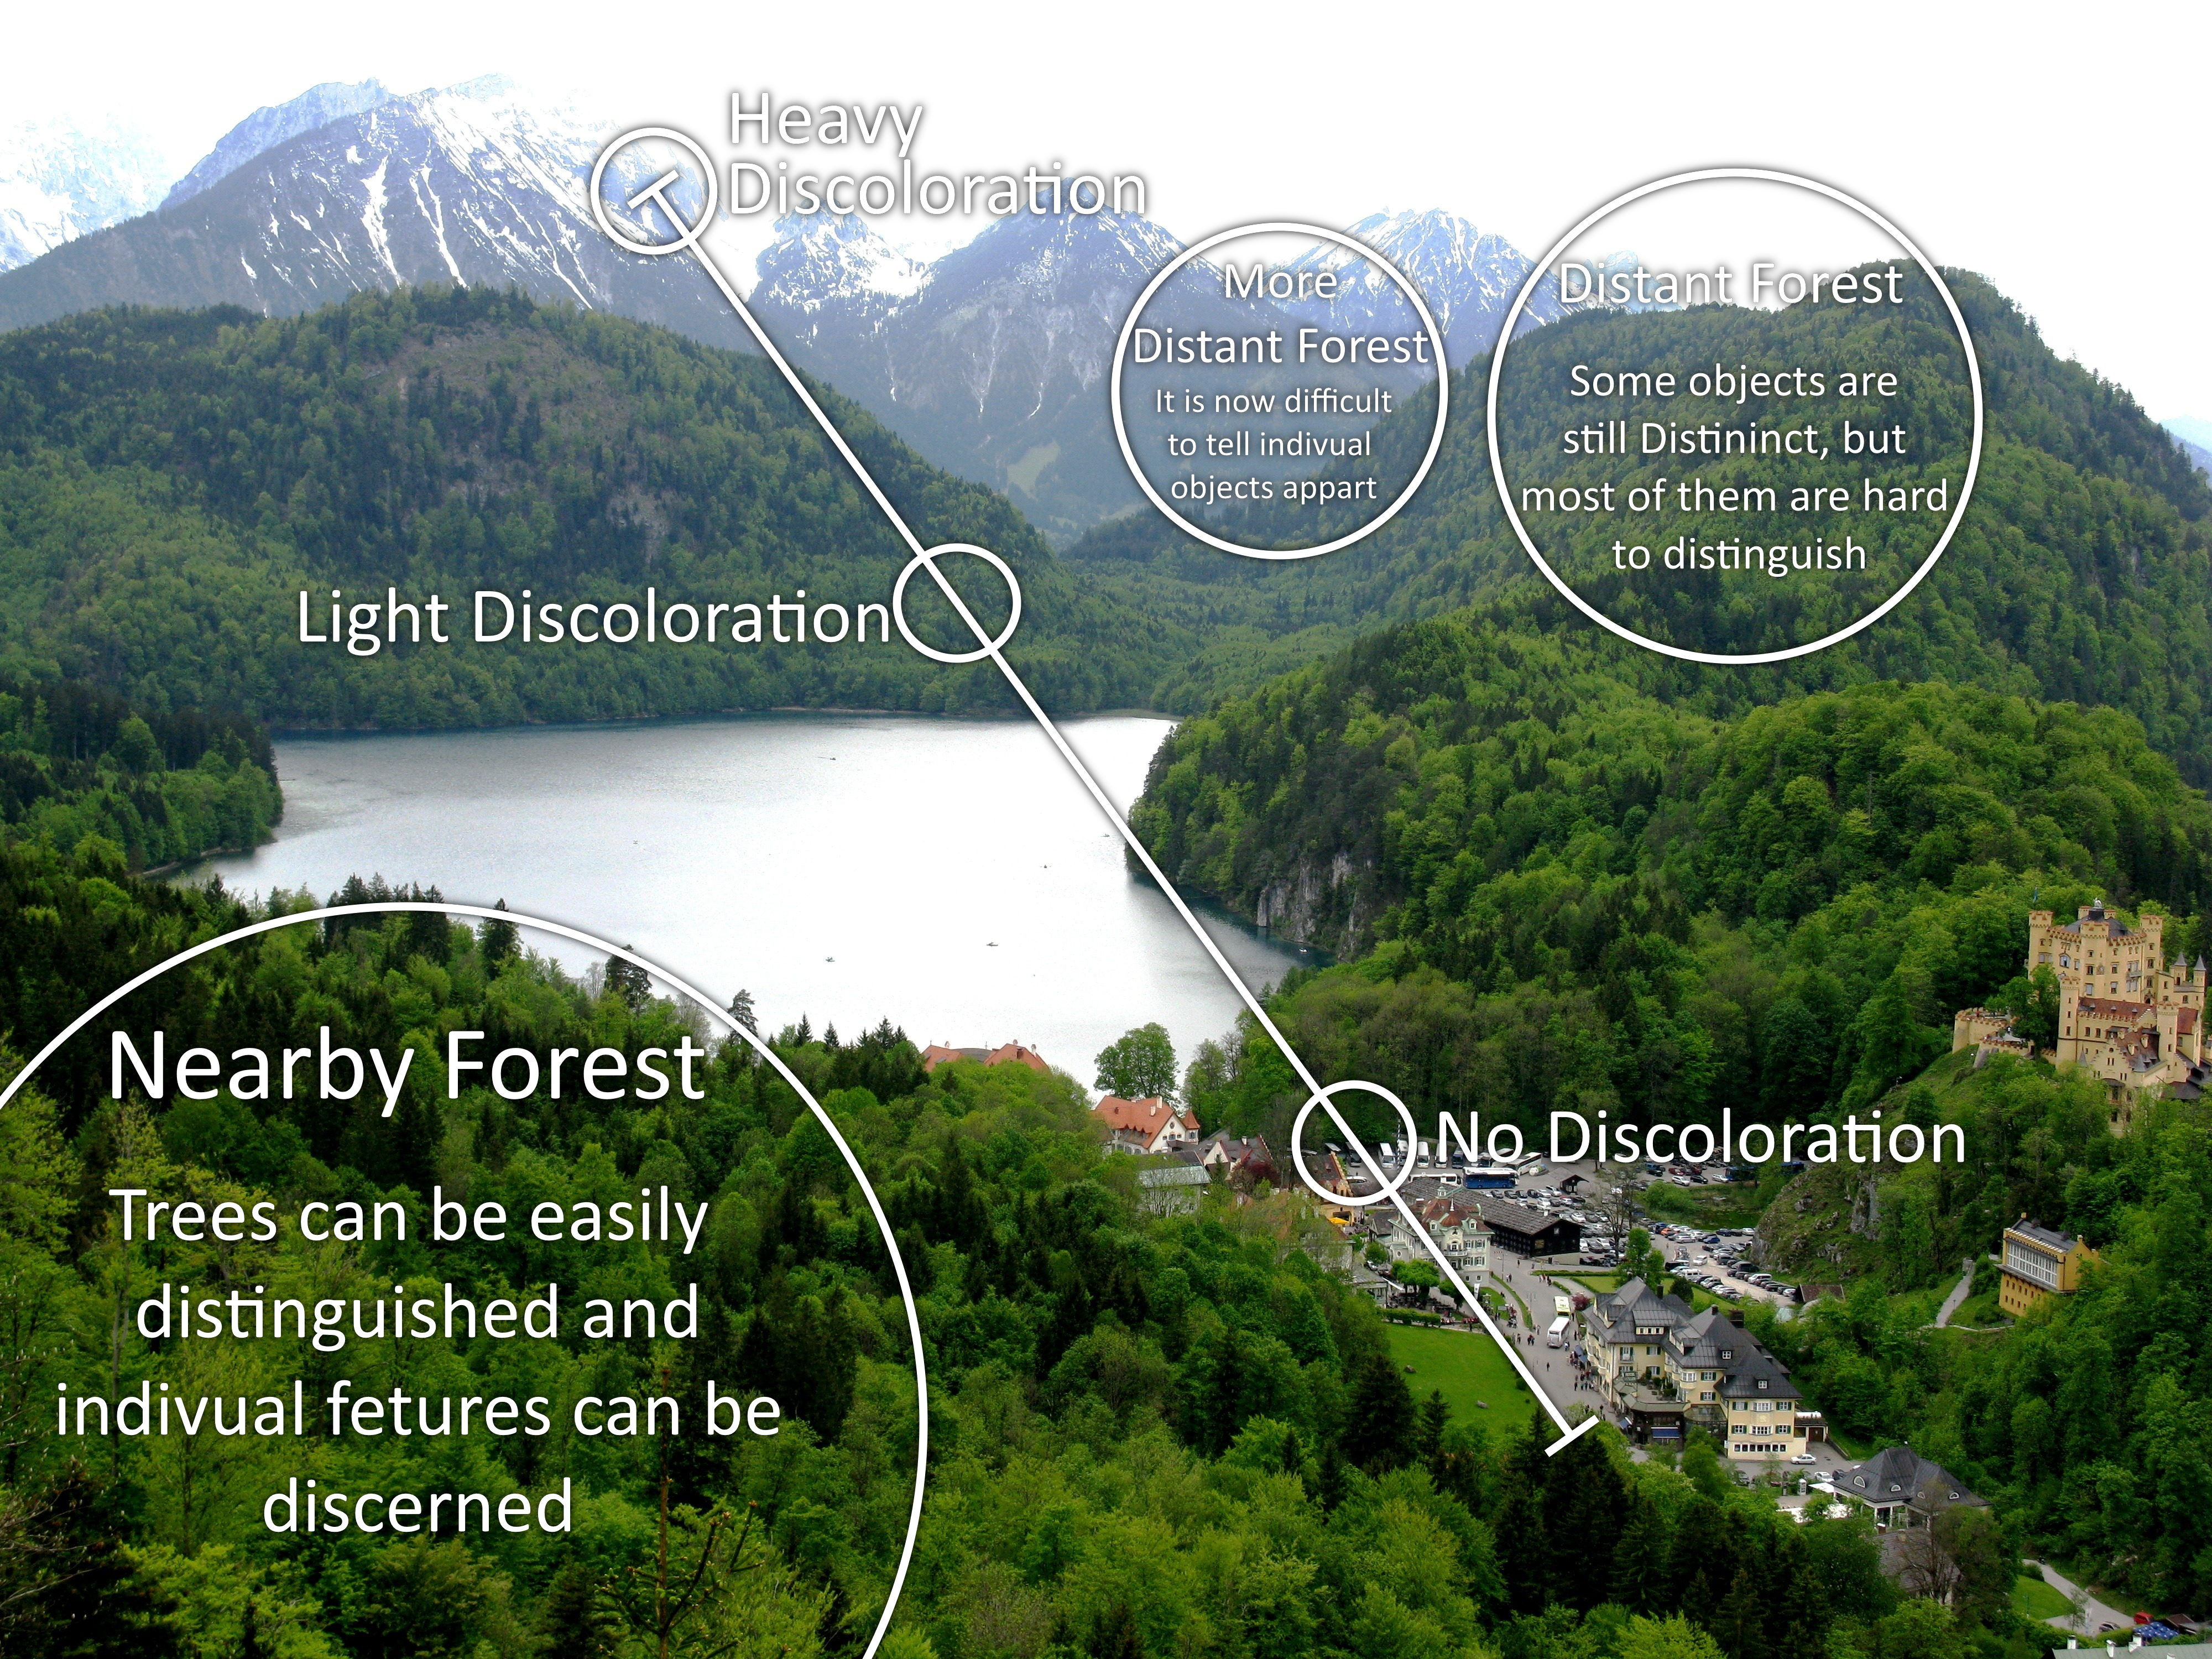
\includegraphics[width=\columnwidth]{Chapter2/Images/RelativeDensityAndAerialPerspectiveExample.png}
    \caption[Aerial Perspective, Relative Size, and Relative Density: An Image of a mountain view in Bavaria, Germany, with indicators to explain how monoscopic depth perception functions]{
        Aerial Perspective, Relative Size, and Relative Density: An Image of a mountain view in Bavaria, Germany. Several circles whose depths indicate how forests are viewed at various depths are shown. A line showing the gradual effects of the aerial perspective is also shown, indicating how it can be utilized to determine depth.
        The background image is licensed under a Creative Commons Attribution Universal 1.0 International license. 
        \footnotemark
    }
    \label{fig:RelativeDensityAndAerialPerspectiveExample}
\end{figure}

Aerial Perspective Refers to our ability to look through transparent objects. Generally, this refers to one's ability to look through the water in the air, making mountains look blue, and is also applicable underwater and when viewing gas-like elements~\cite{Vishton1995}.
Transparent objects can be pretty rare, so most of these elements will naturally be seen from a distance in \autoref{fig:RelativeDensityAndAerialPerspectiveExample}. 
This, however, may not be the need to be the case when using computer graphics~\cite{Vishton1995}.

\begin{figure}[tb]
    \centering
    \includegraphics[width=\columnwidth]{Chapter2/Images/Frenchetal.png}
    \caption[Depth Cues and Motion: Schematic illustration of motion components arising from observer translation and scene-relative object motion.]{Depth Cues and Motion: Schematic illustration of motion components arising from observer translation and scene-relative object motion~\cite{French2022}. (a) An observer fixates on a traffic light while moving to the right, as a car independently moves left. (b–d) Depiction of the car's image motion components related to self-motion and object motion. (d) accounts for image inversion by the eye's lens. (b) If the car is stationary, it shows a leftward image motion due to the observer's movement. (c) If the car moves left while the observer moves right, the car's image motion also includes an object motion component. (d) The net image motion of the car, vret, is to the right. This figure is licensed under a Creative Commons Attribution license and was produced by French and Deangelis~\cite{French2022}.}
    \label{fig:FrenchEtAl}
\end{figure}

\footnotetext{\url{https://pxhere.com/en/photo/965104}}
Motion parallax is considered the depth cue relating to how we perceive motion. 
This seems foundational to how we perceive depth~\cite{Lee1980}.
As seen in \autoref{fig:FrenchEtAl}, the motion perspective normally relies on the user viewer focusing on an object that is moving concerning them~\cite{French2022}. 
This could be looking at a ball they are about to catch or a house in the distance while a user passes it in a car or some other form of transport~\cite{French2022}.
Motion is an effective depth cue within 15 meters, but as \autoref{fig:CuttingDepthGraph} illustrates, the effectiveness lessens when the objects are further away from the viewer and declines when an object is within 2m of a viewer as they can't fully perceive the object~\cite{Shojiro1991}. 

People determine the depth perception of objects based on how their eyes are focused, which can also be a useful depth cue~\cite{Zannoli2016}.
\autoref{fig:AccomodationAndConvergenceInRealAndVirtualWorlds} illustrates how changing the accommodation and convergence allows us to focus on a given object.
Humans can change the disposition between their eyes~\cite{Berkeley1948}. 
Accommodation relates to the ability to change the shape for focus. 
Of the eye to see an object clearly and at different distances. 
Whereas convergence relates to the ability to turn the eyes to focus on nearby objects inwardly. 
These eye movement behaviours have a limited range, \autoref{fig:CuttingDepthGraph} shows at closer distances to us, this depth cue works the most effectively together, but it also shows as the eyes move farther apart, objects positioned further in front of or behind the focal point become increasingly blurred~\cite{Bajura1992}.

% needs a conclusion paragraph to this section
\begin{figure}[tb]
    \centering
    \includegraphics[width=\textwidth]{Chapter2/Images/AccomodationAndConvergenceInRealAndVirtualWorlds.png}
    \caption[A depiction of how convergence and accommodation work in the real world using Mixed Reality and OST AR.]{Convergence and Accommodation:
        A depiction of how convergence and accommodation work in the real world using Mixed Reality and OST AR. It consists of 4 diagrams showing how accommodation and convergence work together to better perception. The blured ducks indicate a point where a duck would not be in focus to the viewer based on the position sitting in this position due to the effect of convergence and accommodation. The frames below show examples of the resulting perceived images of the objects in each diagram. Each of the four diagrams showcases a human eye (the circular object) viewing some ducks. The point where the eyes meet is their vergence or the point of convergence (depicted by the line). The cone represents the accommodation, which focuses on the physical distance the viewer is from the display. This image was inspired by work by Rosedaler. This is licensed under a Creative Commons Attribution licence~\footnotemark.
    }
    \label{fig:AccomodationAndConvergenceInRealAndVirtualWorlds}
\end{figure}

Since both eyes have a different view of the real world, the image each eyes perceive is inherently different.
This enables humans with several different abilities that are processed in the brain: 
\begin{itemize}
    \item \textbf{Stereopsis :} Refers to our human ability to assemble a 3D image from two 2D images from each eye. Giving us the ability to see the world in 3D. 
    \item \textbf{Diplopia :} Also called double vision. This is what occurs with binocular disparity, which can't be completely fixed by Stereopsis, leaving the viewer with two images that are not correctly aligned.
\end{itemize}
These cues give viewers a clear indication of how the world is around them and are referred to in combination as binocular disparities. 
Binocular disparities are more effective when viewed closer to the viewer as the further they are away from each eye, the similar position they are in each eye~\cite{Vishton1995}. 

Other cues can give a viewer a better sense of depth. 
For example, it is possible to directly tell the viewer how far things are by presenting them with a neat grid texture. Explaining to a user exactly how big a world is can obviously present a high level of depth perception. 
Objects with a high amount of contrast can also be clearer to see; however, this can be seen as improving the relief size and density.
Finally, humans may process depth perception in ways we have yet to understand fully; it is quite possible there is an aspect to living on earth, like gravity, that may even have an effect on our sense of depth perception~\cite{Vishton1995, Watson1992}.

\footnotetext{\url{https://commons.wikimedia.org/wiki/User:Rosedaler}}

\subsection{Research into the Depth Perception of Color}
This dissertation utilizes several colorful objects in its evaluations and creates two studies that directly utilize someone's ability to discern color from a specified area. 
This particular section highlights the papers of note that researched the impact of colors on depth perception.
By understanding this research, the changes in depth perception that various colors can provide were mitigated across this dissertation. 

Ping et al.~\cite{Ping2020a} highlight the impact that colors can have on depth perception.
When talking about medical visualization in general, it is very common to have several transparent layers in a single visualization.
Some research has found that people tend to perceive different colors as being closer or further away than others~\cite{Aoi2020, Ping2020a}.
This section of the thesis discusses the research that has been factored into considerations regarding how color influences depth perception. 

\begin{figure}[bt]
    \centering
    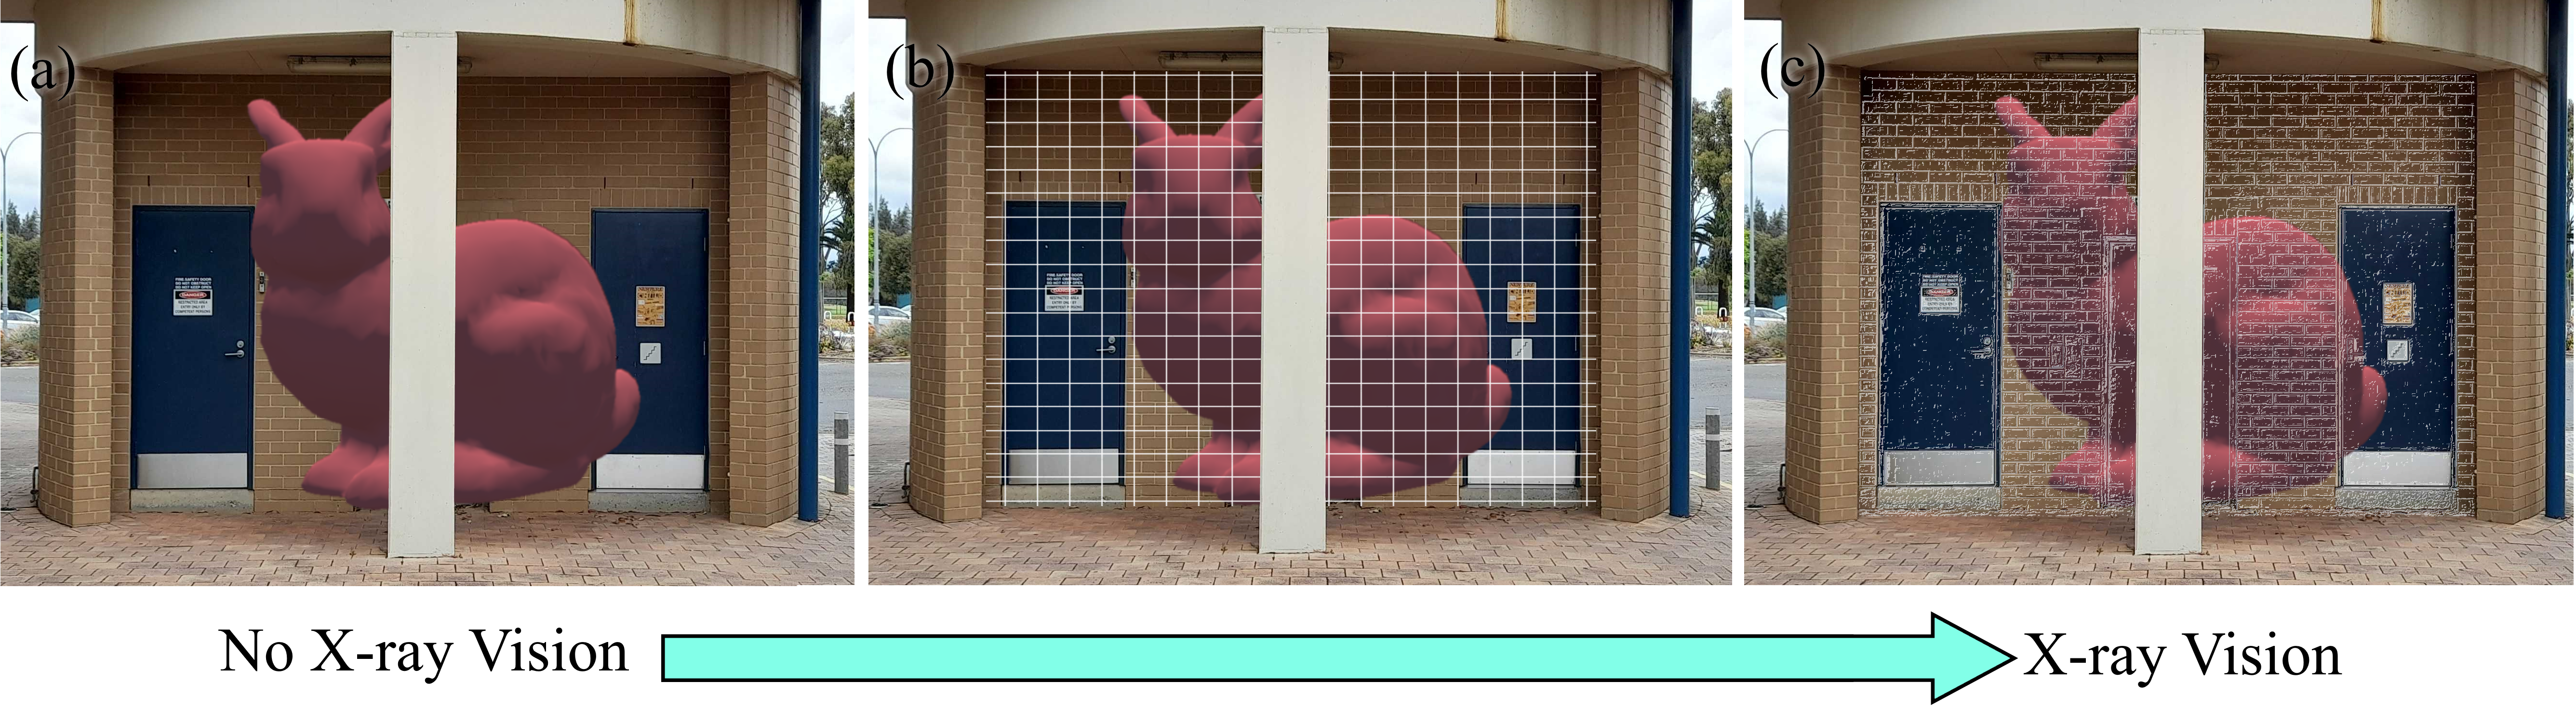
\includegraphics[width=\columnwidth]{Chapter2/Images/ARToXrayVision.png}
    \caption[Three images of the Stanford bunny sitting behind a wall, each using a different \gls{X-ray Vision} effect.]{Three images of the Stanford bunny sitting behind a wall, each using a different \gls{X-ray Vision} effect. To the left, a simple depth cue by placing the bunny behind a column. In the center, a virtual grid is placed over the physical wall to explain to the viewer that the bunny is behind the wall. On the right is highlighting the edge of the bricks with \gls{ar} using edge detection to indicate that the bunny is behind the wall.}
    \label{fig:ARToXrayVision}
\end{figure}

Aio and Li~\cite{Aoi2020} wanted to test how the luminance and Contrast affected the depth perception of transparent plans when viewed on a computer monitor.
The goal was to determine what methods could be utilized to make it more obvious which object was behind the other. 
They had two conditions to achieve this. They utilized luminance contact, testing the difference between changing the gradient between light and dark to dark to light.
They utilized four planes of different sizes to distinguish depth perception. 
This study was conducted using an autoscopic display, which allowed for the presence and absence of motion parallax and no binocular parallax, giving the participants extra depth cues.  
Throughout this study, Aoi and Li~\cite{Aoi2020} noticed participants underestimated depth perception but it could be improved by using either (or both) binocular parallax and motion parallax. 
They also noted that occluding darker or lighter colors did not make much difference.
Aio and Li~\cite{Aoi2020} next utilized the information from their prior study to test this data on medical data and less difference between the choices of different colors. 

\section{Illustrative Rendering Techniques}
Cutting and Vishton~\cite{Vishton1995} claim there are several real-world elements to create depth perception, which then need to be adapted for virtual displays~\cite{Cutting1997}.
However, artists have been able to establish depth perception even when illustrating non-realistic environments by using "Just Enough Reality"~\cite{Siegel2000} to determine depth accurately.

The latter part of this thesis looks at using \glspl{virt} as a method of \gls{X-ray Vision}. 
Building on these perceptual foundations, the challenge in computer graphics—and particularly in advanced visualization domains such as X-ray or mixed reality displays—is not just to replicate the cues found in natural vision, but to enhance and adapt them for clarity and insight. 
While perceptual mechanisms like stereopsis and texture gradients provide a basis for spatial understanding, there are scenarios where simply mimicking the real world is insufficient. 
Here, artistic illustrative effects become invaluable: by deliberately emphasizing, abstracting, or revealing underlying structures, these techniques enable viewers to "see" information that might otherwise remain obscured. 
In this way, the migration from perception-driven rendering toward illustrative approaches is not only a technical evolution, but also a creative one, leveraging artistic conventions to extend the capabilities of visual communication in graphics.


This section is going to look at how these effects have previously been used, what their impact has been on computer science, and what their utility has been when using \gls{mr} devices.
While this thesis only looks into a subsection of illustrative techniques, limiting itself to either Hatching, Stippling, or Halos, the actual definition of this is broader~\cite{Lawonn2018}.
Illustrative techniques can also include the scope of non-photorealistic rendering, like using cell-shading and the deformation of video footage to look like it was produced by a pencil or paintbrush~\cite{Lawonn2018}. 
This section will also examine some user studies that have investigated this effectiveness~\cite{Lawonn2018}. 

The largest examples of illustrative effects being used can be seen in scientific textbooks like Gray's anatomy~\cite{gray1877anatomy}.
This textbook utilized hatching's ability to communicate texture and depth using a black-and-white image.
These images were collected over years of diagramming the human body by directing unclaimed bodies from workhouses and mortuaries. Due to their clarity and accuracy, they are still widely used today. 

Early work in the field by Interrante et al.~\cite{Interrante1995, Interrante1997, Interrante1997a} looked at how illustrative effects can aid the perception of transparent objects.
Transparent objects make it difficult to understand the exact surface of the shape that a transparent object is formed as. 
This was done by pre-computing textures that used transparent and opaque regions.
The first work was done by creating several different textures, including multiple methods that depict valleys and ridges, grids, and curvature information~\cite{Interrante1995}. 

To improve the on their prior work~\cite{Interrante1995}, Interrante~\cite{Interrante1997a} created a visualization that utilized valleys, ridges, and curvature to explain the objects' flow. 
This texture was calculated by drawing lines around the parts of the mesh with the highest curvature and having them move toward the ridges and valleys of the shapes. 
This dissertation extends this research by creating a texture that could be viewed from all sides, requiring less computation when the object is viewed from different angles. 

The textures mentioned in Interrante et al.'s~\cite{Interrante1997} work were later tested with a tipping and a grid-based pattern on each. 
A user study was done to determine if the direction of the lines or opacity affected users' ability to determine the shape of the surface.
At the same time, the participant viewed the graphics on a stereoscopic display. 
This study tested whether participants could accurately determine the closest surface of one noisy sphere to another inside of it. 
The analysis did show that texturing the object improved depth perception compared to a base line condition of having no texturing effect, but there was no significant difference if participants could determine which shell was the closer to themselves. 

\subsubsection{Hatching}

The hatching which was developed in Interrante et al.~\cite{Interrante1997} was later extended by Hertzmann and Zorin~\cite{Hertzmann2000}.
Hertzmann and Zorin~\cite{Hertzmann2000} developed an algorithm that could translate hatching over to smooth surfaces by using a piecewise smooth subdivision to reconstruct a smooth surface from the mesh to compute the necessary qualities.
This allowed for a surface-based rendering technique that worked much like a shadow but also thinned the lines to the point of being invisible when they were in the direct view of the camera. 
They then used a combination of noise generation and denoising functions to create human errors that would be seen in a work of art. 

The system that Hertzmann and Zorin~\cite{Hertzmann2000} created was not designed for real-time interactions.
This means that even simple actions like rotating around the model are not possible. 
Praun et al.~\cite{Praun2001} pre-generated a tonal art map based on different levels and then used these tonal art maps to determine the direction of the hashes before drawing them on the objects themselves. 
This system allowed for a wide variety of different configurations.

This method of hatching was then furthered by Pelt et al.~\cite{Pelt2008} and applied to an iso-surface representing \gls{ct} data.
Their algorithm was modified to consist of just a geometry shader rather than a fragment shader, removing the need for preprocessing the hatching. 
Rather, this system is able to compute the curvature of the iso-surface and an appropriate direction for the hashing in real time while providing a relatively fast frame rate, which would then create a textured striped pattern over a 3D object.

Another system was created by Lawonn et al.\cite{Lawonn2013}, which could run at even faster rates than Pelt et al.'s~\cite{Pelt2008} work as long as it receives extensive pre-processing.
It first identifies key regions: contours, defined by surface normal and view vector perpendicularity, and feature regions, identified by maxima and minima in the mean curvature field.
Then, the direction of the lines is calculated directly from the direction of the curvature.

Hatching effects are also closely tied to brush-like effects, as they require the system to understand brush direction and stroke size. 
Gerl and Isenberg~\cite{Gerl2012} then furthered the possible interactions of hatching and painterly effects. 
This technique preprocessed a \gls{classifier_g} to segment areas of the 3D mesh, then it used a \gls{regression_analysis} to choose the most appropriate direction of the stroke directions.
To aid the AI methods, users were also given several interactions that allowed them to reconfigure the angle and direction of the effect~\cite{Gerl2012}. 

Lawonn et al.~\cite{Lawonn2017} furthered this technique and paired it with a visualization of a cylinder, making the illustrative effects inside of it more apparent than the effects outside. 
The cylinder gave a similar impression to \gls{X-ray Vision}, where the illustrative effects in the cylinder were clear and easy to see, while the effects outside the cylinder were duller. 
The hatching was modified to work on a set of vessels, and the caps of all the vessels and each location where the vessels split were identified so the vessels could be rendered differently.

Lawonn et al.~\cite{Lawonn2017} then ran a study comparing their version of hatching to the same cylinder from their previous study~\cite{Lawonn2017} with pseudo-chroma depth rendering and Phong shading.
Users were asked to define the model's depth tips of two vessels. 
pseudo-chroma depth rendering used the chroma colors to indicate depth, with more saturated colors being closer to the viewer and less saturated colors being further away whereas Phong shading used light and dark to indicate depth.
This study showed that while participants performed faster with the pseudo-chroma depth performed, they were more accurate at assessing the distances and felt more confident in their answers using the hatching condition. 
This shows that hatching may allow for better depth perception. 

\subsubsection{Stippling}
Lu et al.~\cite{Lu2002} furthered the stippling techniques shown by Interrante et al.~\cite{Interrante1997}. 
By looking at the curvature of the model, finding localized curvature of 3D models, and spacing out the dots between the various pixels on the screen. This effect created a realistic stippling effect for 2D images.

\begin{figure}[tb]
    \centering
    \includegraphics[width=\columnwidth]{Chapter2/Images/ImagesFromOtherWorks/PasterAndStrotthote.png}
    \caption[Examples detailing the stippling algorithm created by Pastor and Strotthote~\cite{Pastor2004}.]{Examples detailing the stippling algorithm created by Pastor and Strotthote~\cite{Pastor2004}. The top of this image shows how the stippling subdivision is implemented using a graph function. The bottom image shows an example of how this stippling appears when it is applied to the target object (The bones representing a human hand). A small amount of stipple can be seen on the left of the image where the stipple was evenly and sparsely placed, but there is more depth perception in the center and right images where stippling is more frequent and varied. 
    Used with permission from IEEE \textcopyright{} 2004.}
    \label{fig:PasterAndStrotthote}
\end{figure}

An issue with drawing the dots for stippling was that Lu et al.'s~\cite{Lu2002, Lu20} found that the distance between the dots requires to be randomly placed using a noise-based function rather than just at random. 
It was important space stippling randomly but evenly distributed. 
One solution for this was created by Pastor and Strothotte~\cite{Pastor2004}.
Their version of stippling created a 3D Voronoi pattern over the 3D model, then a graph would be created linking the starting point of all of the dots which shared a boundary. 
This allowed for a seamless decline in the number of \glspl{voxel_g} shown as they would be separated into groups based on the parent-child relationship seen in the upper part of \autoref{fig:PasterAndStrotthote}. 
This enabled the even stippling thresholds seen in the lower part of \autoref{fig:PasterAndStrotthote} creating a sense of depth and shape of the objects it was applied to.

Another way of creating even stippling while allowing for different angles is to utilize a geometry shader to further subdivide the mesh. 
This technique was initially proposed by Meruvia and Pastor\cite{MeruviaPastor2002}.
By doing this, you can subdivide each polygon to give each polygon a set number of dots within it and evenly distribute the dots inside of each polygon.
This system operates under the assumption that areas with more polygons will require a higher density of dots, whereas flat areas will not~\cite{MeruviaPastor2002}.

This method of stippling was later extended by Ma et al.~\cite{Ma2018} to allow for the stippling to be applied to a 3D model in real time that utilized pre-computation to speed up the process rather than a more complex shader.
%Ma et al.~\cite{Ma2018} later created a system to motivate further parts that belonged to be able to move but also by utan utilizing a similar pre-computation to Paster and Strotthote\cite{Pastor2004}.
The dot was placed using blue noise inside the Voronoi, adjusted in size to varying levels, and adjusted in tones based on where they appeared in parallel on the GPU.
This type of stippling allowed for the effect to be placed realistically onto 3D models even as they were changing their shapes. 

\subsubsection{Halo}
Outlines~\cite{Bui2015}, Boundary Enhancements~\cite{Svakhine2003}, feature lines~\cite{Lum2002, Lawonn2015}, and Halos~\cite{Ozgur2017} go by many other names, but they all relate to outlining either individual objects or highlighting areas of very high curvature from the perspective of the viewer. 
With traditional rendering, this tends to be done by viewing the distance between various pixels on the depth map~\cite{Ozgur2017, Lawonn2017} or by calculating the local curvature of the surrounding fragments~\cite{Bui2015, Svakhine2003}. However, this can be very different when working with \gls{dvr} in part to the lack of a defined surface making any surface based calculations challenging.

\subsection{Volumetric Illustrative Rendering Techniques}
In more recent years, many papers have been striving to take volumetric data and present it as illustrative images, with the belief that these images will be easier to communicate and understand in a 2D format.


% Talking about how methods to create these effects for to volumes work:
Initially Interrante et al.'s~\cite{Interrante1997} proposed two methods to convert their illustrative techniques to \gls{dvr}:
\begin{itemize}
    \item \textbf{Scan-Conversion Method: }Converts texture slabs into a grayscale volume. This method is efficient for generating multiple views but compromises stroke crispness due to volume data resolution limitations~\cite{Interrante1997}.
    \item \textbf{Geometric Definition Method: }Directly applies geometrical definitions of strokes during ray casting. This method maintains fine detail but is computationally expensive, requiring repeated intersection tests for each view~\cite{Interrante1997}.
\end{itemize}
Since this thesis is focused on real-time volume rendering for immersive \gls{mr} devices, a new volume was required to be generated each frame. This section will have more of a focus on papers that utilize the Geometric Definition Method. Which has since been heaver extended by other to now utilize techniques that are available on more modern \glspl{gpu} like fragment shaders.

Rheingans et al.~\cite{Rheingans2001} developed a method that was able to separately compute the expected color and the transparency.
This allowed the lighting to react to certain elements and allow different textures within the volume to have a different appearance even if the Hounsfield unit was similar at that \gls{voxel_g}. 
Rheingans et al.~\cite{Rheingans2001} \gls{dvr} algorithm was able to present an accurate texture representation of the various surfaces of the volume and allowed for objects to be presented without regard to density or realism.

Lu et al.\cite{Lu20} created a system that was able to apply stippling to a complete volume. 
This system used algorithms like ray marching similar to \gls{dvr} to perform this calculation.
Visualization focused on rendering the various surfaces to make their curvatures clear but also took into account the amount of density it would have required to reach a given surface. 
Surfaces that were facing the camera were faded out, and the lighting algorithm mentioned in Lu et al.~\cite{Lu20} allowed for shading to become an option to be utilized by the final visualization.

Work done by Bruckner et al.~\cite{Bruckner2007, Bruckner2006} proposed that one method to get around some unwanted details that are an issue with \gls{dvr} would be to utilize non-photo-realistic rendering.
This style of rendering utilized on the surfaces of different objects and rendered them based on their curvature~\cite{Bruckner2006}. 
From this, they developed a simple cartoon-like shading algorithm~\cite{Bruckner2006}, Stippling~\cite{Bruckner2006}, and Halos~\cite{Bruckner2007}.

When volume rendering is utilized in microscopy, it can be difficult to tell the difference between the different boundaries and the elements being visualized. 
Guo et al.~\cite{Guo2012} used a halo visualization to separate the different molecules that can be viewed, as well as two new techniques for promoting contrast in regions of the volume called  Phase Contrast Volume Rendering (PCVR) and Difference Interference Contrast Volume Rendering (DICVR).
PCVR enhances the contrast of almost visible parts of the volume, allowing for a higher contrast.
DICVR tries to extend PCVR further by using interference contrast based on microscopy principles.
They simplified the equation required to create these effects each time by performing multiple rendering passes. 
This work by Bruckner et al.~\cite{Bruckner2007, Bruckner2006} aimed at providing a more simplistic method for creating \gls{dvr} and extending its functionality in biology.

\section{Direct Volume Rendering (DVR)}
The other focus of this thesis is volume rendering. 
Volume rendering relates to the visualization of a volume of data, which is typically created using a \gls{ct} or \gls{mri} machine. However, it can also be used for other scientific visualizations, such as fluid simulations, meteorological data, and geological data. 
Preprocessed Volume Rendering will generally present surfaces of the volumes using polygonal structures utilizing iso-surfaces~\cite{Lorensen:1987:MCA}, but DVR does not require explicit surfaces to be precisely stated. \gls{dvr} can present the data within the natural format as a 3D image~\cite{Drebin1988}.
This allows the system to dynamically represent the volumes from within the system.
However, it does highlight the need for techniques like \gls{ct} and \gls{mri} to be directly aligned with the physical data source. An \gls{X-ray Vision} technique needs to be developed to meet this criterion. 
This section highlights the prior work in this area that influenced the research in this dissertation. 

\subsection{Visualizing Volumetric Data}
Generally, medical volumetric data is viewed using 2D slices of a human body.
After years of training, medical practitioners can be very precise when using these slices, but they are not intuitive to use or to learn how to use~\cite{Cheung2021}. 
Like other forms of 3D data visualizations, converting this data into a 3D version makes it more intuitive to read and interact with~\cite{Jurgaitis2008}. 
This process involves reconstructing 3D models from volumetric data, enabling more intuitive visualization and interaction compared to traditional 2D slice-based approaches.
%As noted earlier, in \autoref{sec:ApplicationsForStereoscopicDisplays} immersive \gls{mr} displays are better suited for helping their users see 3D data. 

\begin{figure}
    \centering
    \includegraphics[width=\linewidth]{Chapter2/Images/Cubrillies.png}
    \caption[A example of Cuberilles.]{A example of Cuberilles. The left side shows the armadillo in its original form. On the right, the same model is rendered using Cuberilles.}
    \label{fig:Cubrillies}
\end{figure}

% numbers in citations are for links to the Marching Cubes paper
Early methods to visualize volumes would focus on calculating the surface contours and calculating the exterior surface to match~\cite{Keppel1975}, which was problematic as it created ambiguity when there were irregularities on the slice data such as those caused by noise~\cite{Fuchs1977}, requiring user intervention to overcome~\cite{Christiansen1978}.
Herman et al.~\cite{Herman1981} tried creating a more automated surface by creating Cuberilles, which functioned similarly to Minecraft blocks~\autoref{fig:Cubrillies}. This was useful as it allowed for varying resolution~\cite{MEAGHER1982129}.
The continuation of this work was marching cubes~\cite{Lorensen:1987:MCA}. Unlike the rough surface afforded by utilizing Cuberilles, this algorithm made a smooth surface.
Marching Cubes utilized the fact that any six \glspl{voxel_g} neighboring \glspl{voxel_g} could be paired into 14 different symmetrical orientations if they were either inside or outside of the threshold.
This made it possible to create a 3D model of a \gls{ct} or \gls{mri} scan with a manageable polygon count that looked similar to the real volume.

% Wünsche~\cite{Wunsche2003} created a system that allows users to view medical 3D data on desktop devices, utilizing bicubic Hermite interpolation with linear interpolation in the radial direction to generate an iso-surface for most models, while the ventricles are created by tracing \gls{mri} contours.
% This system was then paired with a flexible UI, allowing for consistent color representation between models and the ability to incorporate mathematical models to segment the volume. A plane representing the axial and coronal planes also displays the segmented data around the 3D object in 2D.
% A follow-up system to this was later created, which focused on allowing \gls{dvr} to be utilized in a similar format, providing tools to aid users in working with histograms of the volume data while still being able to interact with it in the same math-based manner~\cite{Liu2010}.

Wünsche~\cite{Wunsche2003} introduced a visualization toolkit designed for the exploration of complex biomedical data, with a particular focus on curvilinear finite element data sets. Unlike conventional volume visualization approaches that assume regularly gridded data, curvilinear finite element models define geometry in material space, where grid lines are curved when mapped into world coordinates. The system derives iso-surfaces in material space and then renders them in world space, enabling accurate visualization of organs modelled  using FE techniques, such as the left ventricle of the heart. The toolkit provides several novel features: a modular design for comparing multiple models simultaneously, a generalized field structure allowing the creation and manipulation of scalar, vector, and tensor fields, and boolean filters for segmentation and icon placement. Additional innovations include global color map controls for consistent interpretation across models, and flexible element, plane, and point selection mechanisms. This framework allowed researchers to integrate and explore biomedical data ranging from scalar tissue properties to tensor fields derived from MRI, supporting both quantitative analysis and interactive visualization.

Liu et al.~\cite{Liu2010} extended this line of work by introducing a novel interface for \gls{dvr} aimed at making transfer function design more intuitive and accessible, particularly for non-expert users. Traditional DVR requires carefully crafted transfer functions to map volume data values to color and opacity, a task that can be challenging without specialized visualization knowledge. To address this, Liu and colleagues proposed a spreadsheet-style, constructive visual component-based interface that follows a “programming-by-example” paradigm. Their system automatically analyzes the Douglas–Peucker algorithm~\cite{Douglas–Peucker1973} histograms of the volume data using to detect meaningful structures, from which it generates “unit transfer functions” representing simple, recognizable features. Users can then combine, refine, and merge these units interactively to build more complex transfer functions. Preliminary evaluations demonstrated that even novice users were able to produce meaningful visualizations significantly faster and with less guidance than when using traditional transfer function editors, highlighting the potential of example-based interfaces for democratizing DVR in biomedical applications.

Iso-surfaces are still used widely today as they provide the most efficient means of displaying a shell; however, tasks like diagnostic exploration and interactive tasks are better enabled by \gls{dvr}~\cite{Meissner2000}.
Farrell~\cite{Farrell1983} found a method of using ray casting to create a surface method showcasing one of the first attempts at \gls{dvr}.
However, many of the concepts for this would later be formed by \gls{dvr}, which was initially developed in 1988 by Drebin et al.~\cite{Drebin1988}, who designed this type of visualization as a fix for the all-or-nothing approach that is possible when using an iso-surface. 
Drebin et al.'s\cite{Drebin1988} approach allowed for a realistic, transparent representation of the volume collected from a \gls{mri} or gls{ct} scanner~\cite{Ney1990, Kaufman2000}.
\gls{dvr} functionality was further refined by Engel et al.~\cite{Engel2001} to work with modern equipment. 
Allowing all of the models to be viewed with minimal issues. 
\gls{dvr} rendering was initially only designed for \gls{ct} and \gls{mri} data~\cite{Ney1990, Kaufman2000}, but it was later utilized in other fields.

\subsection{Use Cases for Direct Volume Rendering}

As with many fields, \gls{dvr} can be utilized for education.
MacDougall et al.~\cite{MacDougall2016} provide an example using a large 3D display wall of molecules for chemistry research and education.
These models used the traditional ball on a stick model and \gls{dvr}, which better represented depth and provided a more realistic or cloudy model of the quantum world. 
MacDougall et al.~\cite{MacDougall2016} found that elements of this system could help create new drugs for the future and proposed use cases that would encourage students to become more hands-on.

Hibbard~\cite{HibbardL.1986} talked about how the data from 2D plots is easier to view in 3D when using volume rendering. 
Hibbard~\cite{HibbardL.1986} then also conferred this data could be used to allow this data to be manipulated by using a time-variant, allowing phenomena like the wind to be simple to examine.
These techniques were then extended by Riley et al. ~\cite{Riley2003} to allow for realistic visualizations of cloud maps.
This was impossible using iso-surfaces, which tended to require a form of lighting that clouds did not utilize~\cite {Riley2003}.
~\gls{dvr} allows climate scientists to explore the internal patterns of the effect of time and space on weather phenomena~\cite{Wang2018}.

\gls{dvr} is also used while testing the quality of materials to visulize them. These materials can constis of metals alloys~\cite{Okuyan2014}, minerals~\cite{Okuyan2014} concrete~\cite{Okuyan2014}, resins~\cite{Nguyen2016}, and combinations of different materials used to create a single one~\cite{Groger2022, Okuyan2014}. 
Material science requires understanding materials' internal structures formed under different circumstances~\cite{Groger2022}.
This could be done in the way of running CT scans of being dented or folded, allowing for structural analysis of how different conditions can affect different materials~\cite{Groger2022}.
This can also be applied to the creation of different materials, like sponge-like materials that need to move in certain ways or quantum materials that will arrange atoms, creating some highly precise and gas-like materials~\cite{Okuyan2014, Grottel2012}.
Volume rendering can also be used to show how conducive liquids like resins are moving through non-conductive ones~\cite{Nguyen2016}, allowing for real-time testing of how to develop products using these materials and presenting communication methods with end users~\cite{Nguyen2016}.

Molecular Sciences also use volume rendering to visualize the output gathered from electronic microscopes~\cite{Nguyen2022, Goodsell1989}.
This allows the user to view the contents of a sample collected in 3D based on the different densities, much like \gls{ct} and \gls{mri} data.
Nguyen et al.'s~\cite{Nguyen2022} DiffTEM system adds to this by allowing denoising that utilizes many images of the data collected from different orientations before the data is rendered. 

Geologists can utilize \gls{dvr} to represent the values of radar data~\cite{Baker2007}.
They tend to do this by using ground-penetrating radar~\cite{Baker2007}.
Unlike the previous examples of use cases for \gls{dvr}, radar has many blank areas; Zehner~\cite{Zehner2021} states that \gls{dvr} can be used to both present a more full view of the area but to also better represent the level of uncertainty that can be viewed from this viewpoint.

\subsection{Human Computer Interaction (HCI) Experiments Using Direct Volume Rendering (DVR)}
% Start writing up the separate sections here
Understanding how people visualize or interact with \gls{dvr} is important to this research.
While being able to visualize various data using DVR is one thing, the user experience is more important than the act of being able to display the content because the content rendered by the \gls{dvr} needs to be a more pleasant experience than the alternative situations for it to have utility.
The following section looks at how various studies over time have evaluated systems using \gls{dvr}.

\begin{figure}
    \centering
    \includegraphics[width=\linewidth]{Chapter2/Images/Hui1993.png}
    \caption[Examples of  Hui et al.'s cursors on 3D planes.]{Examples of  Hui et al.'s~\cite{Hui1993} cursors on 3D planes. Right) Nail on plane, where the cursor has the ability to rotate around the volume; Left) Venetain blind, a non-flat plane, which allows the user to navigate easier on all dimensions using the cursor. Used with permission from IEEE \textcopyright{} 1993.}
    \label{fig:Hui1993}
\end{figure}

One of the first instances of human interaction being a concept using \gls{dvr} is the work by Hui et al.~\cite{Hui1993} on a cursor for these interactions.
This cursor is displayed in \autoref{fig:Hui1993} and works similarly to how a mouse works on a 2D plane, but it had the ability to be rotated on another plane using another 1D input, like the scroll wheel on a mouse, to rotate the plane the mouse cursor was sitting on.
To inform the user of the depth of the plane was highlighted on the outside of the volume, and a variation blind effect would be used to prevent the cursor from moving too much while still being able to get everywhere~\cite{Hui1993}. 

Kersten et al.~\cite{Kersten2006} performed one of the first studies ever to be done using \gls{dvr} using a 3D display.
This study was focused on how transparency affected depth perception when using \gls{dvr} on a stereoscopic display.
The type of transparency used was commonly associated with direct volume rendering. 
The study design would slowly rotate a cylinder filled with Perlin noise~\cite{Perlin1989} and then rotate it slowly in one direction.
To tell what direction a cylinder was rotating, users would have to understand the approximate position of elements in the noise.
Participants of this study had to do this when using a mono and stereoscopic display and between various amounts levels of opacity. 
Kersten et al.'s~\cite{Kersten2006} findings showed that \gls{dvr} is much more effective on stereoscopic displays.
This shows that the real use case for these techniques may be within the use of stereoscopic devices. 

Several years later, Kersten-Oertel et al.~\cite{Kersten-Oertel2014} looked at methods to tell depth within a sparse volume rather than an occluded one.
This was in the form of a set of Cerebral vascular volumes. 
Five different depth cues and a baseline were utilized throughout this study: Edge Detection (Halos), Pseudo-Chromadepth, Fog, Kinetic depth, and Stereo Vision.
Kersten-Oertel et al.~\cite{Kersten-Oertel2014} tested a combination of experts and novices separately on two different studies.
All of the studies utilized the same procedure, where two vessels were highlighted, and the participants guessed which one was closer to the participant.
One of these studies utilized each depth cue individually, while the other focused on their different combinations.
Individual Chromadepth, Fog, and Stereo were shown to be much more beneficial than the other cues when shown individually. 
While chroma depth and stereo seem to have showcased the most substantial values for the combination, Kersten-Oertel et al.~\cite{Kersten-Oertel2014} study again shows why Stereo-vision of \gls{dvr} is such a strong depth cue.

Another user study looking into the transparency created by using \gls{dvr} was done by Corcoran and Dingliana~\cite{Corcoran2012}. 
This system used two layers of volume rendering: an outer transparent layer and an inner occluded layer.
By having occluded surfaces, Corcoran and Dingliana~\cite{Corcoran2012} could provide lighting to parts of the volume that were occluded by rendering the image throughout multiple passes.
%From this, they then ran a user study that investigated using the user's preferences to compare their shadowed-enabled volume rendering to a version that didn't have any shadows.

To evaluate the effectiveness of placing shadows in \gls{dvr} Corcoran and Dingliana~\cite{Corcoran2012} ran a series of studies using a computer monitor running at approximately 20fps, each consisting of less than 20 participants.
The first one was designed to test the users' preferences. This was done by having the participants view the same object side by side. Participants were asked to say whether the shadowed-enabled or non-shadowed versions told them more about the volume. 
The next study looked at shape perception, which had participants arrange two images of similar body parts from two different datasets.
This shape perception study showed that raycasted shadows were not essential for shape perception, but instead, the \gls{ui} was because participants were able to orientate their depth perception by with the ability to rotate the object.
The next study looked at relative depth perception. One user chose a point on the screen that was closest to themselves, and they found that showing shadows significantly increased depth perception.
They note here that it was uncommon for participants to answer this incorrectly. 
The final experiment had users determine how far into a volume the point was by having them estimate the location of an artifact inside of the volume. 
This task found that depth perception was not affected by the distance or the presence of shadows inside of the volume; rather, it may hinder the absolute depth perception. 
Overall, Corcoran and Dingliana~\cite{Corcoran2012} show that shadows can help detail information in a Volume, but they don't necessarily improve perception if there are other depth cues present like motion.

Three studies to use \gls{dvr} with \gls{mr} were done by Laha et al.~\cite{Laha2013, Laha2012, Laha2012a, Laha2014} who looked at studies which were focused on determining the immersion of different \gls{mr} devices displaying volumetric information.
To best determine the amount of immersion when using \gls{mr} devices, they enabled and disabled head tracking and limited the area that was displayed to the user to $360^{\circ}$, $270^{\circ}$, $180^{\circ}$, $90^{\circ}$. 
These conditions allowed them to determine the required or appropriate level of immersion that was preferable for each task. 
All of their studies utilized a selection of open-source real-world data to do their studies and utilized a range of different tasks suited for each dataset on each one.
The first study was focused on testing if there was any noticeable benefit to \gls{mr} when needing to utilize a \gls{cave} using the restricted motion tracking~\cite{Laha2012}. 
This study which was focused on restricted head motion caused them to notice that any combination of the two conditions was able to grant better results.
Laha et al.'s~\cite{Laha2013} next study utilized the NVisor SX111 a (\gls{vst} \gls{ar} display) under similar circumstances. 
This study found that the performance of their participants was improved by providing the most immersion possible~\cite{Laha2013}.
The final study ran by Laha et al.~\cite{Laha2014} looked at what happened when iso-surfaces were used as the data set, requiring them to change the tasks required and also had them reintroduce stereo vision back to the conditions. 
This study observed that the combination of all of the results was the most suitable for the tasks required to interact with volumetric data visualizations. 

Afterward, Laha et al.~\cite{Laha2016} created a taxonomy of the different types of tasks that are possible when using \gls{mr}, with the goal of remove the domain dependency that exists with empirical studies.
This was done by consulting 167 people using a questionnaire regarding how this taxonomy should be shaped. 
This was done with the aim to allow basic types of interactions to be considered similar to other types of interactions for different fields. 
These different types were classified as:
\begin{itemize}
    \item \textbf{Searching:} Searching for the presence or absence of an object, or counting the amount of a given object.
    \item \textbf{Pattern Recognition:} Looking for trends like what side of the data set are there more blood vessels or repetition and asking the participant how many times certain items appear.
    \item \textbf{Spatial Understanding:} This section is for tasks that require the participant to understand the orientation or position of a feature in the dataset. 
    %Spatial understanding can be split into three subcategories:
    % \begin{itemize}
    %     \item \textit{Absolute} Participants Locate a feature in the dataset that is the highest, lowest, furthest, etc., from the participant viewpoint or in the dataset.
    %     \item \textit{Reative:} Participants Judge if one feature in the dataset is in front, behind, higher, or lower than another object.
    %     \item \textit{Intersection:} Participants are asked if two objects are intersecting with each other. 
    % \end{itemize}
    \item \textbf{Quantitative Estimation:} These focus on tasks that have the users estimate the properties of a feature of the dataset. 
    \item \textbf{Shape Description:} Requires the user to describe a shape they are viewing. 
\end{itemize}
They also note two possible viewing styles: Egocentric and exocentric. They also note how the different dimensionality of the data should be considered.
Overall, this study paper has informed the design process of the later studies. 

% sketch-based interactions
Sketch-based interactions allow for an easy interaction with volumes.
Shen et al.'s~\cite{Shen2014} split the various use cases this technique could be used into seven different categories: selection, cutting, segmentation, matching, coloring, augmentation, and illustration. 

An early version of volumetric hatching used in this dissertation was inspired by research from Feng et al.~\cite{Feng20152548}, which helped establish fundamental approaches to illustrative rendering.
Feng et al.~\cite{Feng20152548} created a system that projected a grid over the area of the volumetric area.
This was chosen to help highlight objects and clearly present the depth to different areas when faced with users who do not understand the depth of objects within the volume.
This system worked by projecting a 2D grid on the first available \gls{voxel_g} in the ray marching algorithm when it was in the range of the grid texture. 
They note in their findings that chroma color could be utilized to highlight depth perception.

\begin{figure}
    \centering
    \includegraphics[width=\columnwidth]{Chapter2/Images/ImagesFromOtherWorks/Grosset.png}
    \caption[
            The 6 datasets used in Grosset et al.'s~\cite{Grosset2013} research.
        ]
        {
            The 6 datasets used in Grosset et al.'s~\cite{Grosset2013} research: (a) aneurysm, (b) backpack, (c) bonsai, (d) flame, (e) Richtmyer-Meshkov instability \& (f) thorax. Used with permission from IEEE \textcopyright{} 2013.
        }
    \label{fig:Grosset}
\end{figure}

Almost all interactions with \gls{dvr} require good depth perception, even when they are using a 2D display. 
Grosset et al.~\cite{Grosset2013} created a user study that aimed to test if the depth of field could be utilized with \gls{dvr}. 
This study looked at replicating a person's ability to focus on an element based on how deep it was in the volume that they were focused on.
This was tested using a Dynamic and a Static experiment. 
The static experiment asked participants to judged which of two circled features in still images was closer in depth, testing whether Depth of Field and projection type affected speed and accuracy.
The Dynamic Experiment required participants to watch short videos where the focal plane swept through the scene and then judged which circled feature was closer, testing whether dynamic focusing improved depth accuracy.
The Dynamic Experiment allowed the user to control the depth of field by tracking their eyes. 
The other experiment by Grosset et al.~\cite{Grosset2013} set the focal points at the most optimal place.
While there was not much difference between the different conditions, both studies provided similar answers.
Whether this technique was static or dynamic didn't make much difference between various conditions. 
However, they did notice a difference between the different sets of data shown in \autoref{fig:Grosset}.
Each different dataset which was visualized had a different amount of depth perception, with the bonsai and thorax datasets being the easiest to determine depth, while the flame and Richtmyer-Meshkov instability datasets were the hardest to determine depth.
This was likely because each dataset they utilized presented a vastly different type of visualization, which utilized different depth cues to various levels~\cite{Grosset2013}.

Roberts et al.~\cite{Roberts2016} investigated the impact of different types of reconstruction filters for \gls{dvr} graphics using a questionnaire.
%The different reconstruction filters they used as the conditions for their study were: b-spline, Trilinear, CatMull-Rom, Int B-spline, and Welch.
These reconstruction filters included B-spline, Trilinear, CatMull-Rom, Int B-spline, and Welch filters.
Participants were asked to view several open-source datasets and rate their depth quality, layout, sharpness, and jaggedness. 
This paper did not have many major findings. B-spline was preferable for the tasks they suggested but not to a significant amount. 
What was interesting about this research was that the datasets seemed to have more of an impact than the conditions themselves did, much like Grosset et al.'s~\cite{Grosset2013} study.

\begin{figure}
    \centering
    \includegraphics[width=\columnwidth]{Chapter2/Images/ImagesFromOtherWorks/Englund2018.jpg}
    \caption[Conditions used in Englund et al.'s~\cite{Englund2016, Englund2018} studies.]{Conditions used in Englund et al.'s~\cite{Englund2016, Englund2018} studies.
    (a) Direct Volume Rendering (DVR), (b) Depth of Field, (c) Depth Darkening, (d) Volumetric Halos, (e) Volume Illustration, and (f) Volumetric Line Drawings. Used with permission from John Wiley and Sons \textcopyright{} 2016}
    \label{fig:Englund2018}
\end{figure}

To get around the issue of not being able to create a sated by Roberts et al.~\cite{Roberts2016} and Grosset et al.'s~\cite{Grosset2013}, Englund et al.~\cite{Englund2016, Englund2018} created 15 volumetric images in the shape of a cube and took photos of each of the sides these volumes, which allowed them to take 90 images of different volumes, which they then utilized in a questionnaire.
%A sample of these volumes can be seen in ~\autoref{fig:Englund2018}.
They then took these images with six different \gls{dvr} visualization techniques seen in \autoref{fig:Englund2018}
~\footnote{The descriptions used in Englund et al.'s~\cite{Englund2016, Englund2018} may be misleading when compared to other research. So the names they have used are in parenthesis.} : Depth Darkening (Depth Darkening),
Depth of Field (Depth of Field), 
Subtractive Color Blending (Volumetric Halos), 
Additive Color Blending (DVR), 
White Outlines(Volumetric Lines), 
Toon Shading (Depth Darkening), 
Black Outlines(Volume Illustration).
This questionnaire had participants perform \gls{twofc} questionnaire for multiple depth perception studies if participants could visually orient the images in the same positions and how attractive the different conditions they presented were~\cite{Englund2016}.
This study found that depth darkening and Halo's gave the best sense of depth perception out of all the conditions, and the occlusion cue-in seems to be the most effective way to determine depth perception based on it. Orienting the shapes was easiest to determine using the toon shading, as that method highlighted the shapes of the foreground objects the best. Most users preferred depth darkening~\cite{Englund2016}. 

The Englund et al.'s~\cite{Englund2018} study design and conditions were later consulted on by three experts. 
This clearly explains both the Subtractive Color Blending and Black Outlines. 
One main issue an expert noted was that as these sources of data only represented a single image, they didn't accurately represent the interaction that people would have with volume data, as this was expected to be utilized to properly view the data, like being able to rotate the volume. 
The same expert noted that the Toon shading hid aspects of the volume due to its high opacity.
One expert noted that the outlines would be better suited if they could react to the surfaces's outline.
Some of the most important expert findings from Englund et al.'s research~\cite{Englund2018} was that by highlighting the edges of the objects, depth perception was most improved by communicating to the user where the front and back of the objects were. 
These factors likely were likely why the black outlines performed as well as they did.


\section{An introduction to Augmented Reality (AR) and Virtual Reality (VR)}
% Millgrims AR
Augmented Reality or \gls{ar} refers to the ability to bring virtual objects into the real world \cite{Milgram1994}.
\gls{ar} technologies are part of Milgram et al.'s~\cite{Milgram1994} Mixed Reality Continuum (seen in \autoref{fig:MillgirmsMixedReality}), which represents the spectrum of technology that can augment the visual world. 
The more of the world that is the viewer's perception is moved towards only being able to sense the virtual world the more further along the scale it becomes until a user is fully immersed in a virtual world. 
%\gls{ar} refers to the ability to bring virtual objects into the real world by overlaying them on someone's vision.
\gls{mr} talks about the spectrum between the real and virtual worlds, not including them. 
Resulting in \gls{mr} to include many different types of displays, given the types of interactions ranging from \gls{hmd}s, \gls{cave}s, Handheld Devices, \gls{sar} displays, and even some large monitors can be used as mixed reality devices. 

\begin{figure}
    \centering
    \includegraphics[width=\textwidth]{Chapter1/MillgirmsMixedReality.pdf}
    \caption{A simple view of Milgram et al.'s Mixed Reality Continuum~\cite{Milgram1994}.}
    \label{fig:MillgirmsMixedReality}
\end{figure}

\subsection{Mixed Reality (MR) Hardware}
% Why is this section needed
This section covers the relevant hardware for this dissertation, focusing on devices that provide an \gls{mr} experience to gain an understanding of the experiences that are relevant and that combine real-world interactions with computer graphics.
%Medical, \gls{X-ray Vision} applications and Depth Perception studies have been developed for a large plethora of devices that can be found all across Milgram's~\cite{Milgram1994} Mixed Reality Continuum.
These devices have been designed for different applications and, as such, have different strengths and weaknesses across Milgram 's~\cite{Milgram1994} Mixed Reality Continuum.
This section focuses on the advantages and disadvantages of the hardware used in the relevant research for this dissertation. 

% Talking about the first AR and VR paper
%In 1968 AR
The first \gls{ar} system (seen in \autoref{fig:TheSwordOfDamaclies}) was created by Ivan Sutherland in 1968 "The Sword of Damocles"~\cite{Sutherland1968}. 
This modified a person's sight by adding computer graphics to it. 
By tracking where the user moved their head every 10ms, the system would update the images that the system presented to them within 3D space.
The position of the user's eyes in each lens would determine the direction of the 3D object, which was tracked by a collection of exterior sensors placed around the space users could walk around~\cite{Sutherland1968}.

\begin{figure}
    \centering
    \includegraphics[width=\columnwidth]{Chapter2/Images/TheSwordOfDamaclies.PNG}
    \caption[Ivan Sutherland's~\cite{Sutherland1968} "The Sword of Damocles" one of the first head-mounted \gls{ar} systems.]{Ivan Sutherland's~\cite{Sutherland1968} "The Sword of Damocles" one of the first head-mounted \gls{ar} systems. This image is a reprint published by~\cite{Baus2014} licensed under a Creative Commons Attribution licence. Permission of the original image is granted to make digital or hard copies of all or part of this work for personal or classroom use is granted without fee, provided that copies are not made or distributed for profit or commercial advantage.}
    \label{fig:TheSwordOfDamaclies}
\end{figure}

% the implications of Sutherlands system. 
Sutherland's~\cite{Sutherland1968} Sword of Damocles became the progenitor of all modern \gls{ar} and \gls{vr} \glspl{hmd}. 
In the following decades, researchers developed methods to interact with computers using hand gestures~\cite{Pizer1986} to interact with 3D desktop displays and found cheaper and more ergonomic ways to present this information~\cite{Wang1990}.
Research was done to shrink the size of these displays into a more portable size~\cite{Mann1997}.

% What is augmented Reality Used for
\gls{ar} can be found in many different industries~\cite{Park2021}.
Entertainment and gaming use \gls{ar} to create an experience that is based on navigation like Ingress or Pokemon Go~\footnote{\url{https://pokemongolive.com/}}, also first-person shooters, puzzle games, and board games~\cite{Park2021, Marto2022}.
Industrial maintenance uses \gls{ar} to instruct people on the maintenance of complex machinery~\cite{Kim2018}, 
Tour Guides use \gls{ar} to guide users around cities and buildings and to explain the contextual information to the end user ~\cite{Kim2018}.
\gls{ar} is also being used to extend existing telecommunications technologies, allowing volumetric communications to be possible between different groups of people~\cite{Kim2018}.

% An overview of smartphone technology
Modern smartphones and tablets provide a suitable platform for presenting video see-through mixed reality experiences that use the smartphone's camera to capture the physical world, which is augmented with digital content. The wide availability of smartphones has also made them a popular choice for \gls{mr} experiences. 
One advantage of this approach is the display's brightness, which often outperforms head-worn displays that can appear washed out compared to head-worn displays.  
Mobile devices don't provide an immersive experience; smartphones need to be held by the user, and they can allow for an \gls{ar} experience or require a stand during the operation. A use case that has been gaining popularity is for training or education applications where 3D content is presented as an adjunct to a paper-based medium.

% An overview of SAR-based systems
Projector-based mixed reality systems, also known as \gls{sar}, employ projectors to alter the appearance of physical objects that can be highly organic in shape instead of a typical projector screen. This form of augmented reality has received less attention compared to head-worn and hand-held solutions. However, projected information provides some unique features that have the potential for several applications. An advantage of projected information overlaid on physical objects is that multiple observers can be perceived as the same projection simultaneously and from multiple points of view. For example, visualizations of internal anatomical details directly projected onto the human body~\cite{Hoang2017}.

% Explaining caves in some detail
\glspl{cave} environments are another instance of \gls{sar}. Caves are three-dimensional cubicles that use several projected images to simulate an immersive 3D environment without users needing to wear a headset. As such, caves can provide a collaborative \gls{ar} experience for one or more medical professionals who wish to explore vast amounts of information collaboratively. For example, medical data can be visualized in the form of three-dimensional models that can be viewed collaboratively in a cave environment for diagnosis~\cite{Knodel2018}. \gls{dicom} files were processed into 3D models using an algorithm that converts voxels to polygons that are refined into visualizations to be viewed using 3D glasses in a collaborative environment.

% Talking about what are Head-mounted displays
\glspl{hmd} rely on placing the display of the headset as close to the user's line of sight as possible. 
They allow users to move around the virtual content and interact with it naturally through head movement. This offers a means of presenting mixed or virtual reality content suitable for medical visualizations, training, step-by-step guidance, and many other applications~\cite{Park2021, Ding2022}. 
Since Ivan Sutherland's \gls{hmd} in 1968~\cite{Sutherland1968}, it has been iterated on since, especially in the last several years since VR headsets have drastically lowered in price and become a consumer commodity~\cite{Xie2021, Ding2022}. 

% What is virtual reality
\gls{vr} \glspl{hmd} are available in many different forms. They are accompanied by supporting technologies such as position tracking, front-facing cameras, eye tracking, EEG sensors, and hand controllers to deliver compelling virtual experiences~\cite{Lee2008}. 
Desktop systems such as the Oculus Rift S and HTC Vive Pro offer high-quality display systems that, coupled with a high-end PC, present immersive 3D environments in real time. They also incorporate tracking systems that enable hand-held controllers to support interactions in virtual worlds. Standalone hardware options such as the Oculus Quest and Vive Focus have also become available, removing the need to be tethered to a PC and allowing for wide-area virtual environments to be configured. One of the advantages of head-worn displays is that they leave the operators’ hands free to perform other tasks, unlike hand-held technologies, such as smartphones, which require the user to hold the device during operation.

% Introduction into ocular see through 
\textbf{\gls{ar} \glspl{hmd}} tend to come in two distinct types: 
\gls{vst}, and \gls{ost} \gls{hmd}s. 
\gls{vst} \gls{hmd}s use exterior sensors (usually a camera) and an occlusive headset (typically a VR headset)~\cite{Zhan2020, Geng2013, Xiong2021}. 
While \gls{ost} \gls{ar} use a range of different transparent displays.

% Augmented Reality
There have been ongoing improvements in these devices' quality, ergonomic design, resolution, and capability. Early consumer-level displays, such as the Sony Glasstron (1996), provided an augmented reality display solution connecting to a desktop computer. 
This has since been taken to utilizing a Mobile platform with the Microsoft HoloLens (2016).
The HoloLens allowed the user to move around untethered and interact with the virtual environment. 
The system was able to react to the real-world environment, and it allowed for precise (~1.5 cm) spatial tracking.

% An explanation of Augmented Reality HMD's
\gls{ost} \gls{ar} \gls{hmd}s like the Microsoft HoloLens~\cite{microsofthololens} can also be used to display \gls{ar} content within the user's field of sight.
Objects should be locked into place in the real world, allowing users to move around the 3D virtual content while being able to view the real-world content. 
The HoloLens uses environmental information to locate the real world and brings virtual objects into the user's field of view. 

\subsection{Designing Applications for Stereoscopic Displays} \label{sec:ApplicationsForStereoscopicDisplays}
\gls{ar} devices require different types of interfaces based on the required context and functionality~\cite{Karambakhsh2019, Kim2022}.
This section presents design considerations that are important to understand when creating a display that accommodates \gls{X-ray Vision} in a medical setting, which is a key use case for this thesis. 

In their review by Akpan and Shanker~\cite{Akpan2019}, they investigated 3D data visualizations displayed on \gls{vr} headsets compared to 2D displays. 
This review presented studies that tested 3D visualizations identifying key performance elements:
\begin{itemize}
    \item Data can be easier to analyze with visualizations and promotes more experimentation with data sets in the correct situations. 
    \textit{This can be seen in Cordil et al.'s~\cite{Cordeil2017} work where users are encouraged to move around the different axes of graphs to create new ones, encouraging data analysis on a different level. Allowing for a rapid visual analysis with clear results};
    \item Aiding users in understanding the data at a faster rate. \textit{Tanagho et al.~\cite{Tanagho2012} has found that when guiding people using 2D and 3D interfaces for performing a Laparoscopic surgery, participants were faster and more accurate when using a 3D interface compared to a 2D one};
    \item Verifying data using a 3D format can help users to more rapidly verify models. \textit{Majber et al.~\cite{Mujber2004} found this to be the presenting simulation data to stakeholders for factory designs and layouts. The Interface and data visualized by the \gls{vr} device were understandable even to people who were not knowledgeable about the products or factories};
    \item The overall presentation of 3D data tends to be able interpreted more intuitively than 2D models such as graphs or slices. \textit{Qu et al.~\cite{Qu2010} found this when they were simulating the growth of an eggplant, where they found the simulations were made much easier to understand when the user was presented with a 3D graphic of an approximation of the predicted growth of the plant rather than 2D graphs}.
\end{itemize}
Similar findings can also be found in McIntire et al.'s ~\cite{McIntire2012} literature review on the utility of stereoscopic displays compared to conventional monoscopic displays.
McIntire et al.'s ~\cite{McIntire2012} found that stereoscopic display either improved or made no difference in spatial awareness, spatial understanding, classifying objects, spatial manipulation, navigation, and educational activities. 
There is evidence that 3D information made sense when viewed via a stereoscopic display.


Guo et al.\cite{Guo2019} noted that even if a \gls{vst} \gls{ar} \gls{hmd} could be perfectly calibrated to the real world, it still made surgeons nervous to really on an external device connected to the \gls{hmd} via a wired or wireless connection, because it could lose its calibration making the system inaccurate, or it could turn off and occlude the surgeon's vision altogether.
Andrews et al.~\cite{Andrews2021} note in their literature review that due to the HoloLens's gesture controls allow for operations within sterile environments. 
Making the headset functional in a clinical or surgical setting. 
When Rodrigues et al.~\cite{Rodrigues2017} asked two surgeons how best to create an \gls{mr} sweet of tools. 
Rodrigues et al.~\cite{Rodrigues2017} spent several months talking with two surgeons to choose the best hardware. 
Both opted to use the HoloLens over all other hardware choices.
Pratt et al.~\cite{Pratt2018} utilized the HoloLens to perform several surgeries where the patients \gls{ct} and \gls{mri} data was laid over the top of the patients. 
It is for these reasons that the research in this dissertation chose to use an \gls{ost} \gls{ar} \gls{hmd} (a HoloLens2) for this research.

\subsection{Volume Rendering In Mixed Reality}
Graphical capabilities on \gls{mr} \glspl{hmd} require more simultaneous processes than on traditional displays as they as they require the rendering of multiple displays which need to be redrawn from a slightly different angle each frame, eliminating current hardware acceleration approaches~\cite{Geng2013}.
This is made much harder as many modern \gls{ost} \gls{ar} headsets utilize mobile hardware even to produce the most simple 3D visualization~\cite{Zari2023}, resulting in only a few papers on this topic.
Authors have, however, found ways of getting this technique to function on \gls{mr} \glspl{hmd} by utilizing external devices and optimizing rendering through specialized GPU pipeline~\cite{Mejias2025,Gao2025}.
This has made possible research that spans gamification, medical assistance, collaboration, and high-fidelity graphics interaction, resulting in some interesting features.

% extend this part Ross note

\begin{figure}
    \centering
    \includegraphics[width = \columnwidth]{Chapter2/Images/ImagesFromOtherWorks/Cecottietal.png}
    \caption[The virtual scene created by Cecotti et al.]{The virtual scene created by Cecotti et al.~\cite{Cecotti2021} (a) the 3D data, (b) the sagittal (y-z), (c) coronal (x-y), (d): transaxial (x-z) planes. Used with permission from IEEE \textcopyright{} 2021.}
    \label{fig:Cecottietal}
\end{figure}

Gamification is often used to increase student retention in education. 
One system created by Cecotti et al.~\cite{Cecotti2021} allowed students to learn how to read medical images using 3D spaces as well as 2D ones. 
The scene shown in \autoref{fig:Cecottietal} shows the information presented to the students and how it allows them to map individual planes to a 3D object, allowing them to learn how various organs are seen using 2D planes.
This is currently integrated into their institution's anatomy curriculum.

Pelanis et al.~\cite{Pelanis2020} asked a series of surgeons to compare how using a 3D rendering of \gls{ct} data compared to a more traditional 2D representation of the same \gls{ct} data when using an \gls{ost} \gls{ar} \gls{hmd}.
The \gls{ct} data consisted of images of 150 different legions. 
The medical practitioners correctly accessed 89 of the 150 legions using both formats, and there was no real difference in the accuracy of the visualizations.
There was a difference between the time required, where MRI scans required an average time of 23.5 sections, while the \gls{ost} \gls{ar} \gls{hmd} only took practitioners an average of 6 sections to diagnose.
Pelanis et al.~\cite{Pelanis2020} highlights that there is still an advantage to using 3D graphics even when a person is highly trained. 

Cinematic Rendering is generally a costly method of viewing Volumetric data. It cannot be run in real time and requires a very powerful computer. 
Stadlinger et al.~\cite{stadlinger2021cinematic, Stadlinger2019} utilized a workaround for this method where they took many images of the volume and rendered them on 2D planes for the user to see.
This allowed this technique to be viewed using a lowered-powered machine. 
This made the processing so efficient that Steffen et al.~\cite{Steffen2022} could display cinematic rendering on the \gls{vr} headset.

Steffen et al.'s~\cite{Steffen2022} research had ten trained medical investigators look at ten patient cases using both a desktop display and \gls{vr} \gls{hmd}. 
When these users were asked to assess the volume details, they were more accurate when using a desktop. 
They also noted that desktop displays offered better depth perception when viewing cinematic rendering.

Heinrich et al.~\cite{Heinrich2021} performed a series of tests looking at the difference between depth perception between \gls{ar} and \gls{vr} when looking at volumetric vascular structures rendered as an iso-surface.
They then utilized three different depth cues: Phong Shading, pseudo-chroma depth shading, and surrounding the volume with a Fog.
Users would be presented with a set of spheres located at the ends of all of the blood vessels and asked if they could sort them from nearest to farthest.
Using Pseudo-Chromadepth shading or Fog techniques clearly improved desktops, as these showed the z-axis. 
However, VR users rarely make any errors. 
This was because they could freely use an array of other depth perception cues, such as Convergence, Binocular Disparities, Motion Perspective, and even, in the case of Fog and Aerial Perspective. In contrast, the desktop was limited to Occlusion, Real Size, and Density, which any display could also use.
However, this does show that just using a \gls{ar} device will improve the depth perception of a task using volume data, but it also indicated that the need limits required for testing medical data needed to become much more precise than before to enable the type of accuracy required by the medical field.

\section{Augmented Reality Enabled X-ray Vision} \label{sec:BackXRayVision}
One important aspect of \gls{ar} enabled \gls{xray} vision relates to the field of research looking at aligning the depth mismatch when virtual objects are placed inside of physical objects in \gls{ar}. 
As is shown in \autoref{fig:ARToXrayVision} since \gls{ar} superimposes the virtual objects over the real world it is difficult to make them look like they are behind an occlusive surface. 
It is to this end that many \gls{X-ray Vision} effects have been developed for different devices to solve these issues. 

The goal of this research is to determine methods where \gls{X-ray Vision} effects can work with \gls{dvr} on \gls{ost} \gls{ar} \glspl{hmd}. 
To ensure that this research in this dissertation has a solid basis for the lessons learned by the previous works, a systematic literature review was conducted. %An overview is provided in \Cref{app:XRayLitReviewMethodology}.
This literature review was inspired by the PRIMA 2020 SRC (Page et al. 2021) protocols checklist. It utilized five databases: 
ACM Digital Library~\footnote{\url{https://dl.acm.org/}}, 
IEEE Xplore~\footnote{\url{https://ieeexplore.ieee.org/Xplore/home.jsp}}, 
Pub Med~\footnote{\url{https://pubmed.ncbi.nlm.nih.gov/}}, 
Web of Science~\footnote{\url{https://www.webofscience.com/wos/}}, 
and Scopus~\footnote{\url{https://www.scopus.com/}} 
using the search terms:
\textit{“("X-ray vision" OR "X-ray visualization" OR ("occlusion" AND "perception") OR (visualization AND x-ray) OR "see-through vision" OR "ghosted views" OR "augmented reality x-ray") AND ("AR" OR "Augmented Reality" OR "Mixed Reality")”}
These terms were filtered by the paper’s Abstract, Title, and Keywords. A backwards and forwards snowball was conducted where each papers citations and references where each checked for overlaps on to the existing papers selected for the study which then produced either caused the final search to be adjusted (to the one mentioned earlier). Each time the search criteria was changed the search would begin again. If the papers were not located in the databases listed (grey literature) would be added if they passed all criteria and where papers cited by more than five papers were also considered for entry into this database (2 papers found and accepted). For a paper to be accepted, it needed to meet the eligibility criteria outlined below as determined by the single reviewer. The process and results of this review as depicted in \autoref{fig:X-LItReviewMethodology}

\begin{figure}
    \centering
    \includegraphics[width=\textwidth]{Chapter2/Images/LItReviewMethodology.pdf}
    \caption{The protocol utilized for this literature review with the matching results. }
    \label{fig:X-LItReviewMethodology}
\end{figure}

\subsubsection{Eligibility Criteria}
All papers in this review needed to meet the following criteria:
\begin{itemize}
    \item X-ray vision (XRV) needed to be explored in the research, placing virtual objects behind real-world objects.
    \item Mixed Reality Technologies other than VR must have been used.
    \item Papers that simply superimposed data over the real world and papers that did not focus on making the content appear on the other side of or within the real-world object were not included.
    \item Studies included in multiple papers were only recorded once all papers that highlighted the same research had been included in this review, as the content between both articles provides different amounts of information.
    \item If the focus on XRV was light compared to other study elements and two or more reviewers agreed on it, then the work would not be included in favor of more focused research. 
\end{itemize}

These criteria ensured that the X-ray visualization was more than superimposing a medical image onto a human subject. Any paper that did not utilize \gls{ar} was removed. This meant that some documents that utilized Virtual Reality technologies to test \gls{ar} in a completely virtual environment were not included.


\subsection{Observations from Systematic Literature Review}

\begin{figure}[bt]
    \centering
    \includegraphics[width=\textwidth]{Chapter2/Images/XRayResearchDoneOverTime.png}
    \caption[A bar graph representing the number of papers that were published between 1990 and 2023 focusing on \gls{X-ray Vision}.]{A bar graph representing the number of papers that were published between 1990 and 2023 focusing on \gls{X-ray Vision}, each categorized by the type of research undertaken.}
    \label{fig:XRayResearchDoneOverTime}
\end{figure}

This section presents the complete findings of all the \gls{X-ray Vision} papers that were found as of October 30, 2023. It discusses all the devices on which \gls{X-ray Vision} techniques have been used, along with the techniques for \gls{X-ray Vision}, their functional mechanism, and the research focus. Following this, I looked at how each user study was conducted and the parameters utilized for the various experiments. 

Of all the selected papers that were longer than two pages, 27 Technical papers were found (3 of which also included a case study), and another 29 papers were found that presented a user study. Three demonstrations have been showcased at conferences. Ten short papers have highlighted several methods of research, including a proposal, many of which detail pilot studies for some of the 29 user studies. Every task that required its own set of results was considered a study, and if no results were published for a given study, it was not included in our analysis. 

In recent years, peer-reviewed research proposals have become increasingly common compared to technical papers. Prior to 2010, the literature was predominantly technical in nature. This shift may reflect an evolving trend in the field, where research is expected to address a broader range of topics or where purely technical contributions are less frequently regarded as sufficient on their own. Importantly, research proposals continue to play a valuable role by introducing new ideas and approaches, guiding future investigations, and helping to shape the direction of the field. Over the past decade, our understanding of \gls{X-ray Vision} has advanced through a combination of user studies and research proposals that explore and refine emerging techniques. As shown in \autoref{fig:XRayResearchDoneOverTime}, the field has steadily matured, with a growing emphasis on evaluating the impact of these techniques and improving their effectiveness.

% Peer reviewed research proposals have become more frequent than technical papers in recent times. Papers prior to 2010 tended to be largely technical. This may indicate a new trend in the field where papers need to cover more topics now than previously or the technical reseach in this space may no longer be seen as a signficant contribution. Over the last decade or more, we have learned more about how \gls{X-ray Vision} works by focusing on user studies and research proposals detailing new techniques that might be used. This is detailed in \autoref{fig:XRayResearchDoneOverTime}, which illustrates the steady maturation of the field, moving away from novel techniques to understanding their effects and how they can be improved. 

\subsection{Research Exploring X-ray Vision}

Creating an effective \gls{X-ray Vision} solution for a task requires careful design, construction, and system validation to discover an appropriate balance among the possible solutions to address the challenges related to \gls{ar} and \gls{X-ray Vision} technologies. The literature contains research studies investigating depth perception, spatial awareness, interaction techniques, and usability of \gls{X-ray Vision} systems. \autoref{fig:LitReviewTypesOfResearchVsDevices} shows the prevalence of the different topics in the surveyed literature.

The effectiveness of visualizations and interactions for a given task may depend on the distance of the physical and virtual object(s) from the user. The human eye’s ability to perceive depth and fine detail may vary as a function of distance, and a human’s reach to manipulate physical (and sometimes virtual) objects is constrained by human anatomy. Perception and interaction have been studied in several settings, ranging from within arms’ reach distance to scenarios where distant objects are interrogated and manipulated. Depth perception \gls{ar} and \gls{vr} tend to look at methods of improving the user’s sense of space in an environment. Research into the depth perception of \gls{X-ray Vision} focuses on how to influence the impact on depth perception when looking through an object.

Depth perception and perception, more broadly, have received considerable attention in the research community since accurate depth perception is vital for \gls{X-ray Vision} user experience. 
A key focus of research has explored depth perception in \gls{X-ray Vision} as related to fixing the depth/distance offset caused by trying to place a virtual object on the other side of a real-world object in reference to the user's view point~\cite{Furmanski2002, Ghasemi2018, Sandor2010}. This makes the work in this field done with depth perception different from other forms of research on depth perception. Some works are looking into methods to enhance the depth perception of visualization~\cite{Martin-Gomez2021, Fischer2023}. The major finding that seems prevalent in this field is that partial occlusion is an effective tool to improve depth perception.

\begin{figure}[tb]
    \centering
    \includegraphics[width=\columnwidth]{Chapter2/Images/LitReviewTypesOfResearchVsDevices.png}
    \caption{A plot showing the studies that have been run on \gls{X-ray Vision} by device type.}
    \label{fig:LitReviewTypesOfResearchVsDevices}
\end{figure}

Spatial awareness concerns a user’s understanding of and ability to operate effectively in a physical environment augmented through \gls{X-ray Vision}. Findings in this field generally look at the impacts of using these visualizations on aspects like the general placement of an object or attempt to navigate around a foreign environment~\cite{Heinrich2021, Li2016}. \gls{X-ray Vision} can orient people using exterior landmarks across large buildings~\cite{Dey2012}.

Effective mechanisms to interact with and control an \gls{X-ray Vision} visualization are essential to the effectiveness and usability of an \gls{X-ray Vision} system. Making usability the second largest topic of research in \gls{X-ray Vision}. Creating interaction mechanisms that cater to the combined characteristics of physical and virtual elements in \gls{X-ray Vision} can be challenging. Interaction mechanisms, including gestures, button and menu commands, and eye tracking, have been proposed by Wang et al.~\cite{Wang2022, Wang2023} and Liao et al.~\cite{Liao2023}. 


\subsection{X-ray Vision Techniques}
% Needs to be changed
%Various approaches have been employed to create \gls{X-ray Vision} techniques. 
Partial occlusion is a very depth perception cue, while other techniques rely on other depth cues to allow the user to look through real-world objects such as stereopsis.
There are many variations of these effects; very similar effects have been categorized together in this section and will be discussed as a collection of work.

There are two main categories for \gls{X-ray Vision} effects: ones that typically utilize visualization to present occlusion techniques and others that utilize other cues.
There has been much more research within the visualization category, so this has been split into three different sections: Hole in the World-Based \glspl{X-ray Visualization}, Real-World Overlays, and Computer Vision Techniques.
Splitting the visualizations into these groups allows for a more explicit discussion of how they function in their current form.

\begin{figure}[bt]
    \centering
    \includegraphics[width = \columnwidth]{Chapter2/Images/MiscXRayVision.png}
    \caption[Examples of \gls{X-ray Vision} techniques that don't function using traditional techniques but rather label or indicate where objects should be located.]{
    Examples of \gls{X-ray Vision} techniques that don't function using traditional techniques but rather label or indicate where objects should be located.
    a \& b ) Cote and Mercier's~\cite{Cote2018} underground schematics visualized on the ground;
    c ) Eren et al.'s~\cite{Eren2013} labels designed to tell the user if a objects is above or below the ground;
    d ) Muthalif et al.'s~\cite{Muthalif2022} showcases the labels indicating how far below the ground an object is.
    Permission was granted for images a \textcopyright{} 2018, b \textcopyright{} 2018, and c \textcopyright{} 2022 from IEEE. Figure (d) is licensed under a Creative Commons Attribution licence.
    }
    \label{fig:MiscXRayVision}
\end{figure}

Graphs in this section will note an "other" \gls{X-ray Vision} category. 
These effects are used as baselines for various experiments but do provide an understanding that an object is supposed to be rendered underground. 
These effects include things like presenting a written definition of the location of an object displayed like a sign~\cite{Eren2013}.
Other options are a line between the user and the object~\cite{Gruenefeld2020} or a line between the ground and the object~\cite{Muthalif2022}.
Options that were not included but can give a similar form of information could be considered overlaying the ground with the schematics~\cite{Cote2018}. 
These solutions were not included as even though they gave a clear indication of where the user was, they were all complicated for the user, adding steps beyond looking at a 3D object and determining its location. These solutions make great base conditions as they are flawed and complicated, but they are robust. 

\subsubsection{\gls{X-ray Vision} Effects}
\gls{X-ray Vision} can also be achieved by utilizing other depth cues, such as accommodation convergence, relative scale, and density. 

\paragraph{Auxiliary Augmentation} utilizes the relationship between two objects, employing the depth cues of relative size and density and the effect of motion. 
Using another occlusive \gls{X-ray Vision} technique on one object provides enough information to inform the user of the position of the other object~\cite{Kyto2013}.
Auxiliary Augmentation effect should be possible on a 2D display as it uses relive scale and density as its primary depth cues. Still, it is also made more potent on a stereoscopic display like a \gls{hmd}. 
%By using a stereoscopic display, it should also be possible to utilize depth cues like binocular disparities. 

\paragraph{Vergence} 
\gls{X-ray Vision} is designed to have people change and move their focus away from the foreground to focus on the background image. 
This method simulates binocular distortion. By tracking a user's eyes, it is possible to tell when they are trying to look past an object. 
This can advise what should and should not be kept in view whilst creating and placing objects approximately where the users expect them to be. 
By taking advantage of that, it is possible to blur virtual objects when a user is not looking at them to present a viewing experience similar to real life using Accommodation and Convergence~\cite{Kitajima2015, Dunn2018}.

This effect has not seen widespread use only being utilized by Kitajima et al.~\cite{Kitajima2015} who manually created a depth based AR system where the plans were moved so a user could only focus on one to determine if they could regain tell if what was in front or behind.
This study did not find any significant difference in the depth perception of the objects, but they did note that the users found it easier to focus on one object at a time. 
One possible reason is that Accommodation and Convergence are difficult to track, and off-the-shelf \gls{ar} solutions do not provide this capability. 
%This has led to a relatively low amount of research that has taken use of it. 
It makes it a difficult version of \gls{X-ray Vision} to use fully~\cite{Kitajima2015}. 
%This effect seems more effective when used in conjunction with other \gls{X-ray Visualization}.

\subsubsection{Transparency Based X-ray Visualizations}
One form of \gls{X-ray Vision} used is the ability to adjust the transparency of a part of an image (as seen in \autoref{fig:ComputerVisionEffectsAndTransperency}). 
By configuring the transparency according to the current view, a user can be given the impression that the object is either in the foreground or that the transparency is low enough to feel as if they are looking inside the object.
This form of \gls{X-ray Vision} is called Alpha Blending. 

Three papers~\cite{Kameda2004, Ohta2010, Tsuda2005} have explored Alpha Blending and its possible applications when adapting it to security cameras, allowing for one line of sight to combine the information of several security cameras at once. Rather than having each security camera link to a single screen, their \gls{X-ray Vision} method makes the foreground object more transparent, presenting the content behind them. Early observations of this technique presented better information and insight when looking through buildings. Tsuda et al.~\cite{Tsuda2005} found that this technique works best when paired with another visualization technique. 
The inverse of this has also been used as a visualization technique by making the virtual object less visible when compared to the real world~\cite{Aaskov2019}.

Making the virtual world more transparent can help the user focus on the real world using the \gls{ar} system as a guide. 
This method is commonly used in medicine where users want to use \gls{X-ray Visualization} as a guide while still being able to concentrate on their work since they are not distinct~\cite{DePaolis2019, Erat2013, Pauly2012}.
However, when used from a stereoscopic viewpoint, these transparent effects don't seem to address the depth perception mismatch as they don't provide a clear depth cue to the user. 

\subsubsection{``Hole in the World'' X-ray Visualizations} \label{sec:HoleInTheWorld}
Hole-based \glspl{X-ray Visualization} focus on creating a sense of partial occlusion by allowing a user to look through an object. \autoref{fig:VirtualHoleAndVirtualWindowExamples} depicts the three ways this can has been achieved. 
These methods may use partial occlusion by simply having a user look through a 2D window (\autoref{fig:VirtualHoleAndVirtualWindowExamples} virtual window), while others use tunnelling~\cite{Avery2009} or cutaways~\cite{DePaolis2019, Feiner1992}. 
The most popular of these techniques is creating an open box for people to look into, allowing a sense of how far away the virtual object is placed in a real-life object. 
This provides the impression that the virtual object is inside a real-life object. 
This can be seen in \autoref{fig:VirtualHoleAndVirtualWindowExamples} where the armadillos seem to be sitting inside boxes inside the wall rather than superimposed in front of the wall. 

\begin{figure}
    \centering
    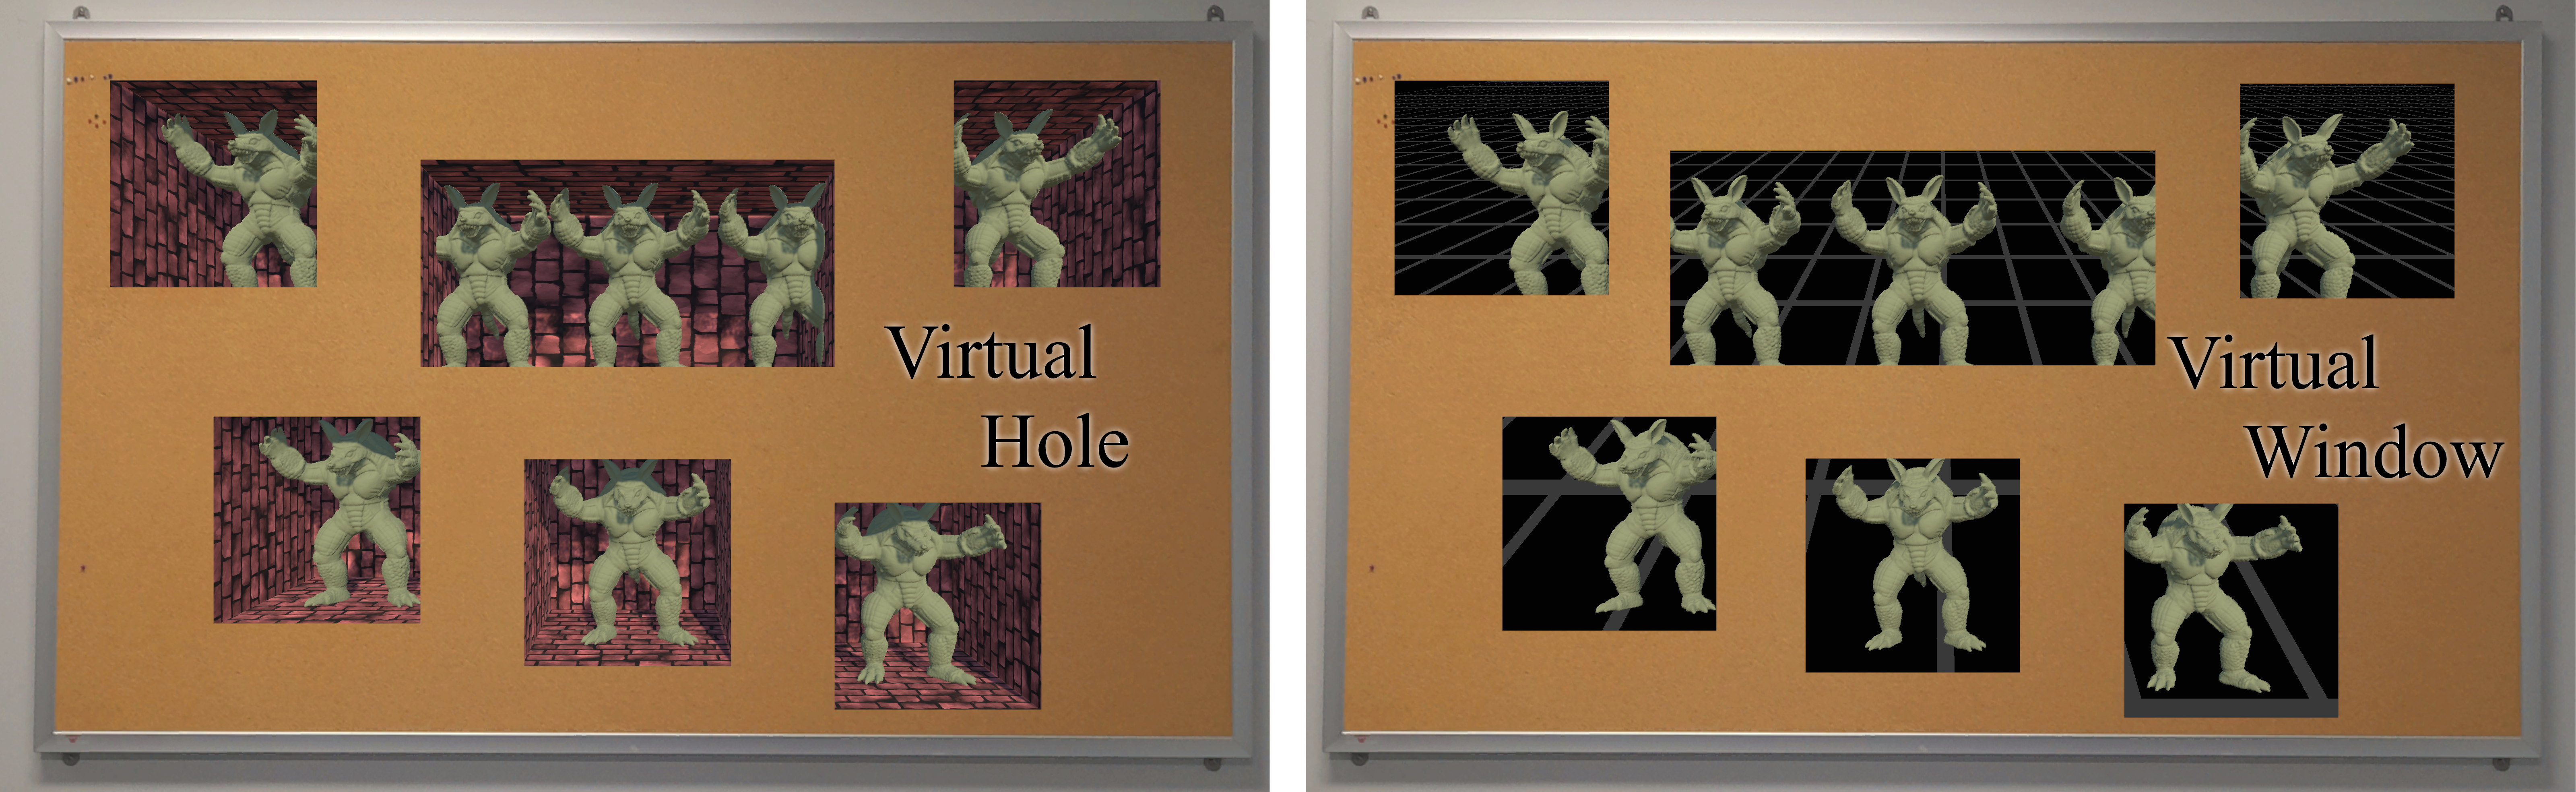
\includegraphics[width=\columnwidth]{Chapter2/Images/VirtualHoleAndVirtualWindowExamples.png}
    \caption[Armadillos sitting behind a corkboard in \gls{ar} with the same orientation using hole-in-the-worlds effects to function.]{Armadillos sitting behind a corkboard in \gls{ar} with the same orientation using hole-in-the-worlds effects to function. On the left are virtual holes, and on the right are virtual windows. }
    \label{fig:VirtualHoleAndVirtualWindowExamples}
\end{figure}

Although hole-in-the-world visualizations work quite effectively utilizing any \gls{ar} display~\cite{Bajura1992, DePaolis2019, Feiner1992, Avery2009, Muthalif2022, Habert2015}, they have a few limitations. Firstly, the visualization needs to be in a static position. 
It cannot rotate or change size relative to the user’s motions, so the hole should not react to the user's position. 
The user could choose to make the hole larger or smaller without breaking the effect. There is a limited field of view into the hole. 
Although the limited view creates the \gls{X-ray Vision} effect, it restricts the user's view of the data. 
One advantage of this \gls{X-ray Vision} method is that it can be viewed using any display.

\paragraph{Virtual Box/Hole:}

\begin{figure}[t]
    \centering
    \includegraphics[width=0.6\columnwidth]{Chapter2/Images/BajuraetalX-ray.png}
    \caption[A image of Bajura et al.'s~\cite{Bajura1992} \gls{X-ray Vision} technique.]{A image of Bajura et al.'s~\cite{Bajura1992} \gls{X-ray Vision} technique. Used with permission from ACM \textcopyright{} 1992. Permission to make digital or hard copies of all or part of this work for personal or classroom use is granted without fee, provided that copies are not made or distributed for profit or commercial advantage}
    \label{fig:BajuraetalX-ray}
\end{figure}

The Virtual hole \gls{X-ray Visualization} was the first type of \gls{X-ray Vision} to be implemented and was designed by Bajura et al.~\cite{Bajura1992} (seen in \autoref{fig:BajuraetalX-ray}). 
Who aimed to visualize a baby fetus inside of its mother's womb.
They accomplished this by presenting a box for the baby to be seen in, which would allow for some level of occlusion.
It is still one of the most used \glspl{X-ray Visualization} and is still being researched in modern studies due to their effectiveness and versatility~\cite{Blum2012, DePaolis2019, Phillips2021}. 
Virtual holes have been found to provide a relationship between virtual objects and the real world. 
%Kytö et al.~\cite{Kyto2013} found that users could better determine distance if they had a partially occluded object in the scene for users to use as a reference.

Research has also observed that introducing some particle occlusion alone may aid depth perception~\cite{Kyto2013}.
It has been observed by Kytö et al.~\cite{Kyto2013} that users could better determine distance if they had a partially occluded object in the scene for users to use as a reference or even using other virtual objects as a reference.
This was demonstrated in a study that partially occluded the edges of other objects and found that as long as some of the \gls{X-ray Vision} effects were covering part of the virtual scene, then it was possible to make smaller objects behind it appear to be a given depth behind as there was another object sitting in the front\cite{Kyto2013}.

\begin{figure}[tb]
    \centering
    \includegraphics[width=\columnwidth]{Chapter2/Images/AvvedutoEtAl.png}
    \caption[This image contains the \gls{X-ray Vision} study environment from Avveduto et al.~\cite{Avveduto2017}.]{This image contains the \gls{X-ray Vision} study environment from Avveduto et al.~\cite{Avveduto2017}. 
    a) shows a study setup that was utilized throughout this study, with the virtual objects present.
    b) shows the no \gls{X-ray Vision} condition used for this experiment from the participant's view.
    c) shows the \gls{X-ray Vision} conditions used for this experiment from the participant's view. 
    Used with Permission from Avveduto et al.~\cite{Avveduto2017}.
    }
    \label{fig:AvvedutoEtAl}
\end{figure}

\gls{sar} \gls{X-ray Vision} techniques papers utilize virtual holes as they work well with \gls{perspective_corrected_projection}~\cite{Avveduto2017, Heinrich2019, Heinrich2022}. 
The initial research in this space looks at what is required for a \gls{sar} based \gls{X-ray Vision} system. 
This was done by Avveduto et al.~\cite{Avveduto2017}, who asked participants to perform a mock biopsy like the one shown in \autoref{fig:AvvedutoEtAl}. 
Participants were then asked to attempt this procedure using either an image of a leathery surface or an image of buttons, which provided two different levels of contrast as backdrops for the virtual hole.
A virtual hole to a virtual hole with an occlusion mask against a baseline.
The authors found that using the occlusion mask and the virtual hole provided accurate results, with participants only being off by approximately 2.5cm (sd = 0.5), whereas in tasks where the participants used no \gls{X-ray Vision} 3cm (sd = 0.5). 


Heinrich et al.~\cite{Heinrich2019} later used virtual holes with \gls{sar} using \gls{perspective_corrected_projection} tested methods to illustrate depth perception with and without stereo vision. 
They compared using the conditions shown in \autoref{fig:Heinrich2019} (Phong Shading, Virtual Mirror, Depth-Encoding Silhouettes, Pseudo-Chromadepth, and Supporting Lines). 
This task asked participants to correctly identify the depth order of the cubes that can be seen in \autoref{fig:Heinrich2019}. 
This research found that the stereoscopic representation of SAR improved all conditions regarding time required and perceived difficulty. 
Pseudo-Chromadepth and Support Lines were the most effective \glspl{X-ray Visualization}, whereas Phong and the Virtual Mirror conditions were the most challenging. 

\paragraph{Cutaways and Tunnelling:}

\begin{figure}[!b]
    \centering
    \includegraphics[width=\columnwidth]{Chapter2/Images/ImagesFromOtherWorks/Heinrich2019.jpg}
    \caption[The conditions used in Heinrich et al.'s~\cite{Heinrich2019} investigation in to \gls{sar} based virtual holes.]{The conditions used in Heinrich et al.'s~\cite{Heinrich2019} investigation in to \gls{sar} based virtual holes. a) Phong Shading. b) Virtual Mirror. c) Depth-Encoding Silhouettes. d) Pseudo-Chromadepth. e) Supporting Lines. Used with permission from IEEE \textcopyright{} 2019.}
    \label{fig:Heinrich2019}
\end{figure}

Cutaways and Tunnelling present a hole through an object, revealing an object on the other side of the object~\cite{Avery2008, Avery2009, Feiner1992}. 
Both these techniques can be seen in \autoref{fig:JustTunneling}. They appear as a box with no back. 
The point of these visualizations is to give the sense of going through a real-world object.
These visualizations focus more on indicating where the data is in the real world rather than giving the user a better sense of depth when looking through a particular piece of data~\cite{Avery2009}.


Avery et al.~\cite{Avery2009} observed a slight offset to the perception of depth when tunneling is used on its own~\cite{Avery2009}. 
This can be improved by combining this technique with either a real-world overlay~\cite{Lerotic2007} or any Computer Vision-Enabled Technique~\cite{Avery2009} on either the front or back to help ground the visualization.
This allowed Avery et al.~\cite{Avery2009} and Lerotic et al.~\cite{Lerotic2007} to give their users the perspective of looking through a wall, whereas~\cite{Erat2018} used a smaller form of this to look through an individual wall. This smaller attempt would be considered a cutaway~\cite{Feiner1992}. 

Cutaways don't appear much in \gls{ar} literature however some notable works exist~\cite{Zollmann2012}. The smaller size of the effect means they may require another visualization to repair the depth offset. However, no research has been done to test whether this could be an issue.
Research from Erat et al.~\cite{Erat2018} did find that cutaways make for a very natural way to look through a wall to interact with something like a drone on the other side when compared to looking at the drone from a first-person's viewpoint, but little else is understood about using cutaways in \gls{ar} for \gls{X-ray Vision}.
When testing this use case, they found that technological limitations still held users back from utilizing \gls{X-ray Vision} to render objects underneath the ground~\cite{Erat2018}.

\begin{figure}[tb]
    \centering
    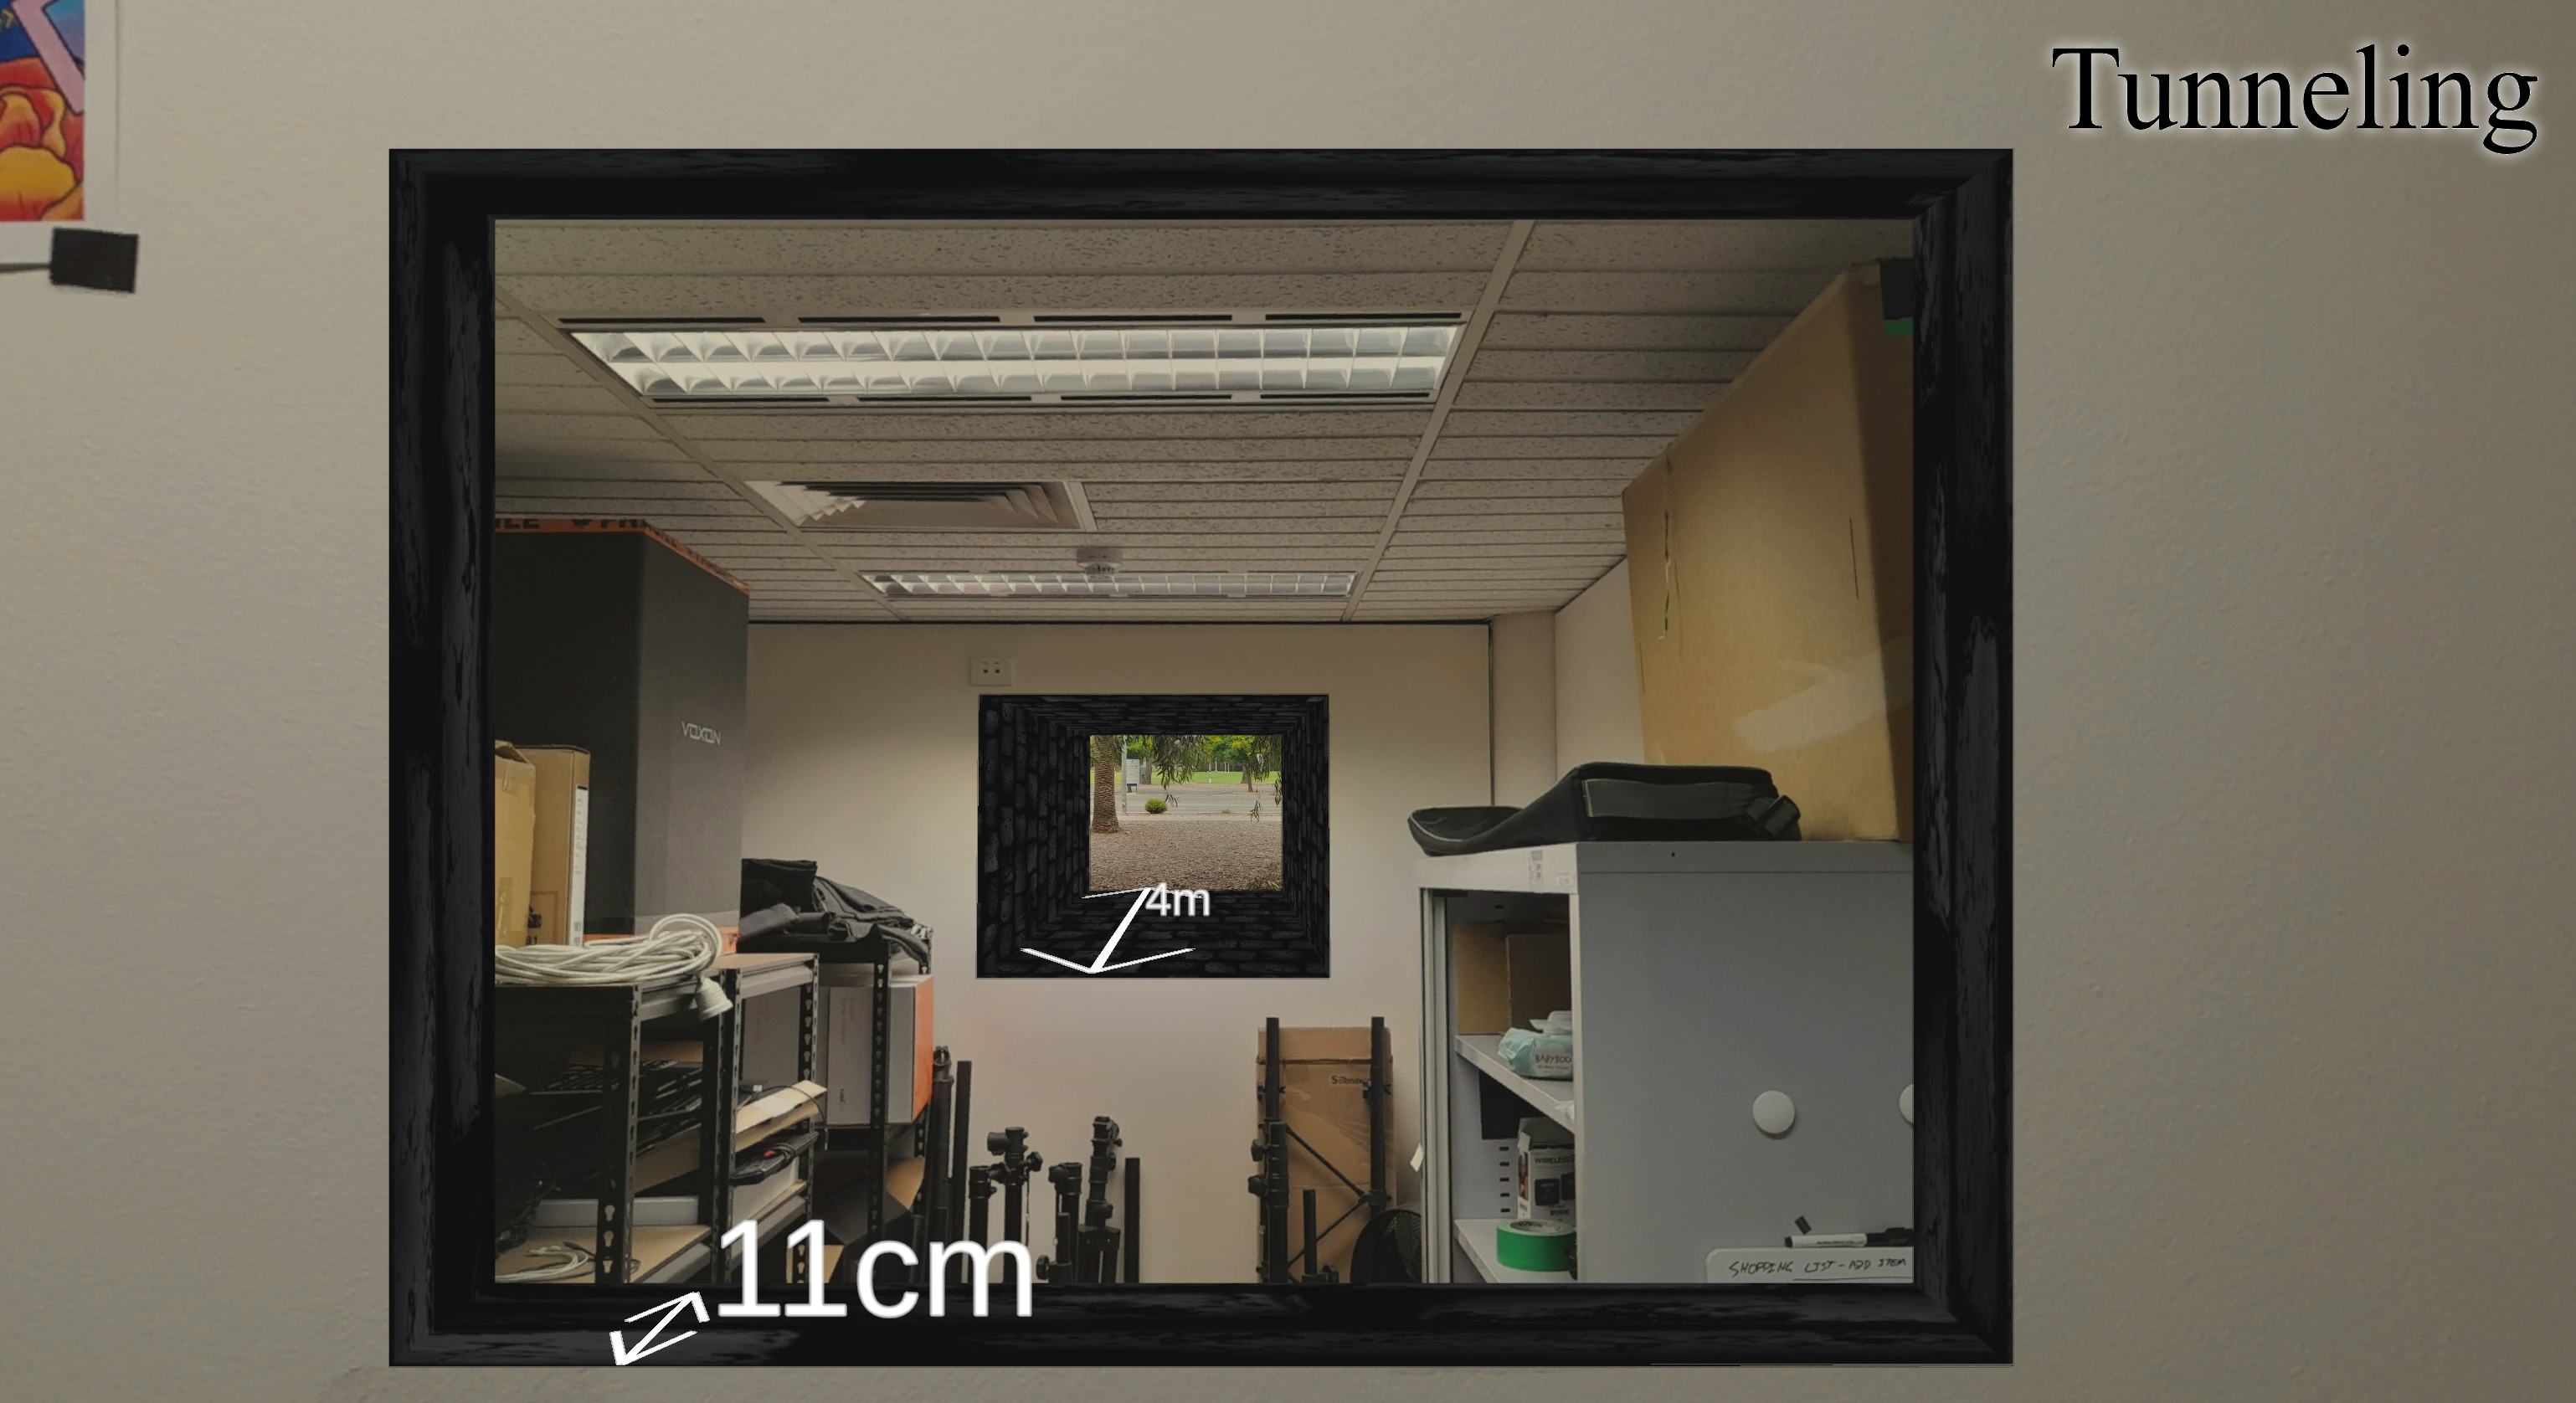
\includegraphics[width=\columnwidth]{Chapter2/Images/JustTunneling.png}
    \caption[A image of the tunneling x-ray visualization used to look through multiple walls.]{A image of the tunneling x-ray visualization used to look through multiple walls. The first arrow looks into a storeroom, whereas the second arrow looks out to the outside. White arrows showcase the depth of the tunnel.}
    \label{fig:JustTunneling}
\end{figure}

\paragraph{Virtual Windows:} 
Virtual Windows shows the user a perspective of a 2D hole in the wall. 
These are sometimes presented as a crack in the wall~\cite{Feiner1992} or will have a slight frame, but what separates this visualization from cutaways is that they ignore the content that is not known and start the virtual space immediately after the real-world surface~\cite{Phillips2022}.
This can be seen in \autoref{fig:VirtualHoleAndVirtualWindowExamples} , merging with the surface of a given material~\cite{Bichlmeier2007, Guo2022}. 

Guo et al.~\cite{Guo2022} utilized virtual holes to enable video games to take place in a \gls{non_euclidean_space}. 
The authors aimed to look at methods where \gls{X-ray Vision} could be made to be more interactive. 
Enabling people to play a game together regardless of their spatial requirements. 
Their experiment had them tag virtual objects that were to tag objects behind the physical walls, which showed to be almost as useful as giving the participants a virtual mini-map with the targets located on it.

Another form of virual windows has been titled "Contextual Anatomic Mimesis" by Bichlmeier et al.~\cite{Bichlmeier2007}. This is one of these windows designed to work autonomously with medical applications. 
The technique that blends virtual anatomical structures with the appearance of real tissue, gradually transitioning from realistic skin to virtual content.
It gradually moves from having the appearance of skin to looking more like the virtual content while still presenting a slight overlay based on the roughness of the skin~\cite{Bichlmeier2007}. 
The effects of Contextual Anatomic Mimesis were furthered by Martin-Gomez et al.~\cite{Martin-Gomez2021}, who have shown a significant improvement when paired with a another second effect to help represent the depth of an object.
Noting that using more than 1 depth cue is beneficial.
These effects ranged from hatching to applying shading to show shadows to the effect where it was found that hatching outperformed the other conditions (hole, ghosted mask, constant, shaded, black, chromatic, and bright)~\cite{Martin-Gomez2021}.
These results have led us to the understanding that illustrative effects may have a slight advantage when providing an understanding of the positioning of data for medical diagrams as they can not only provide a sense of depth perception but are also easy to understand for a general user. 

\subsubsection{Real-World Overlays} \label{sec:realWorldOverlay}
Another way of providing \gls{X-ray Vision} effects is to represent the physical environment using a virtual pattern such as a wireframe or a grid. 
This is typically done in two ways. One way is to place a pattern on the ground, allowing users to retain some knowledge of depth by using a constant geometric cue~\cite{Gruenefeld2020}. The other method utilizes overlaying the real-world object with a pattern of some sort. 
The second method is used when viewing virtual objects in stereoscopic displays, as it requires a level of geometric saliency to be perceptible. 
Binocular disparities are required for these types of visualizations to function~\cite{Otsuki2015}.

\begin{figure}
    \centering
    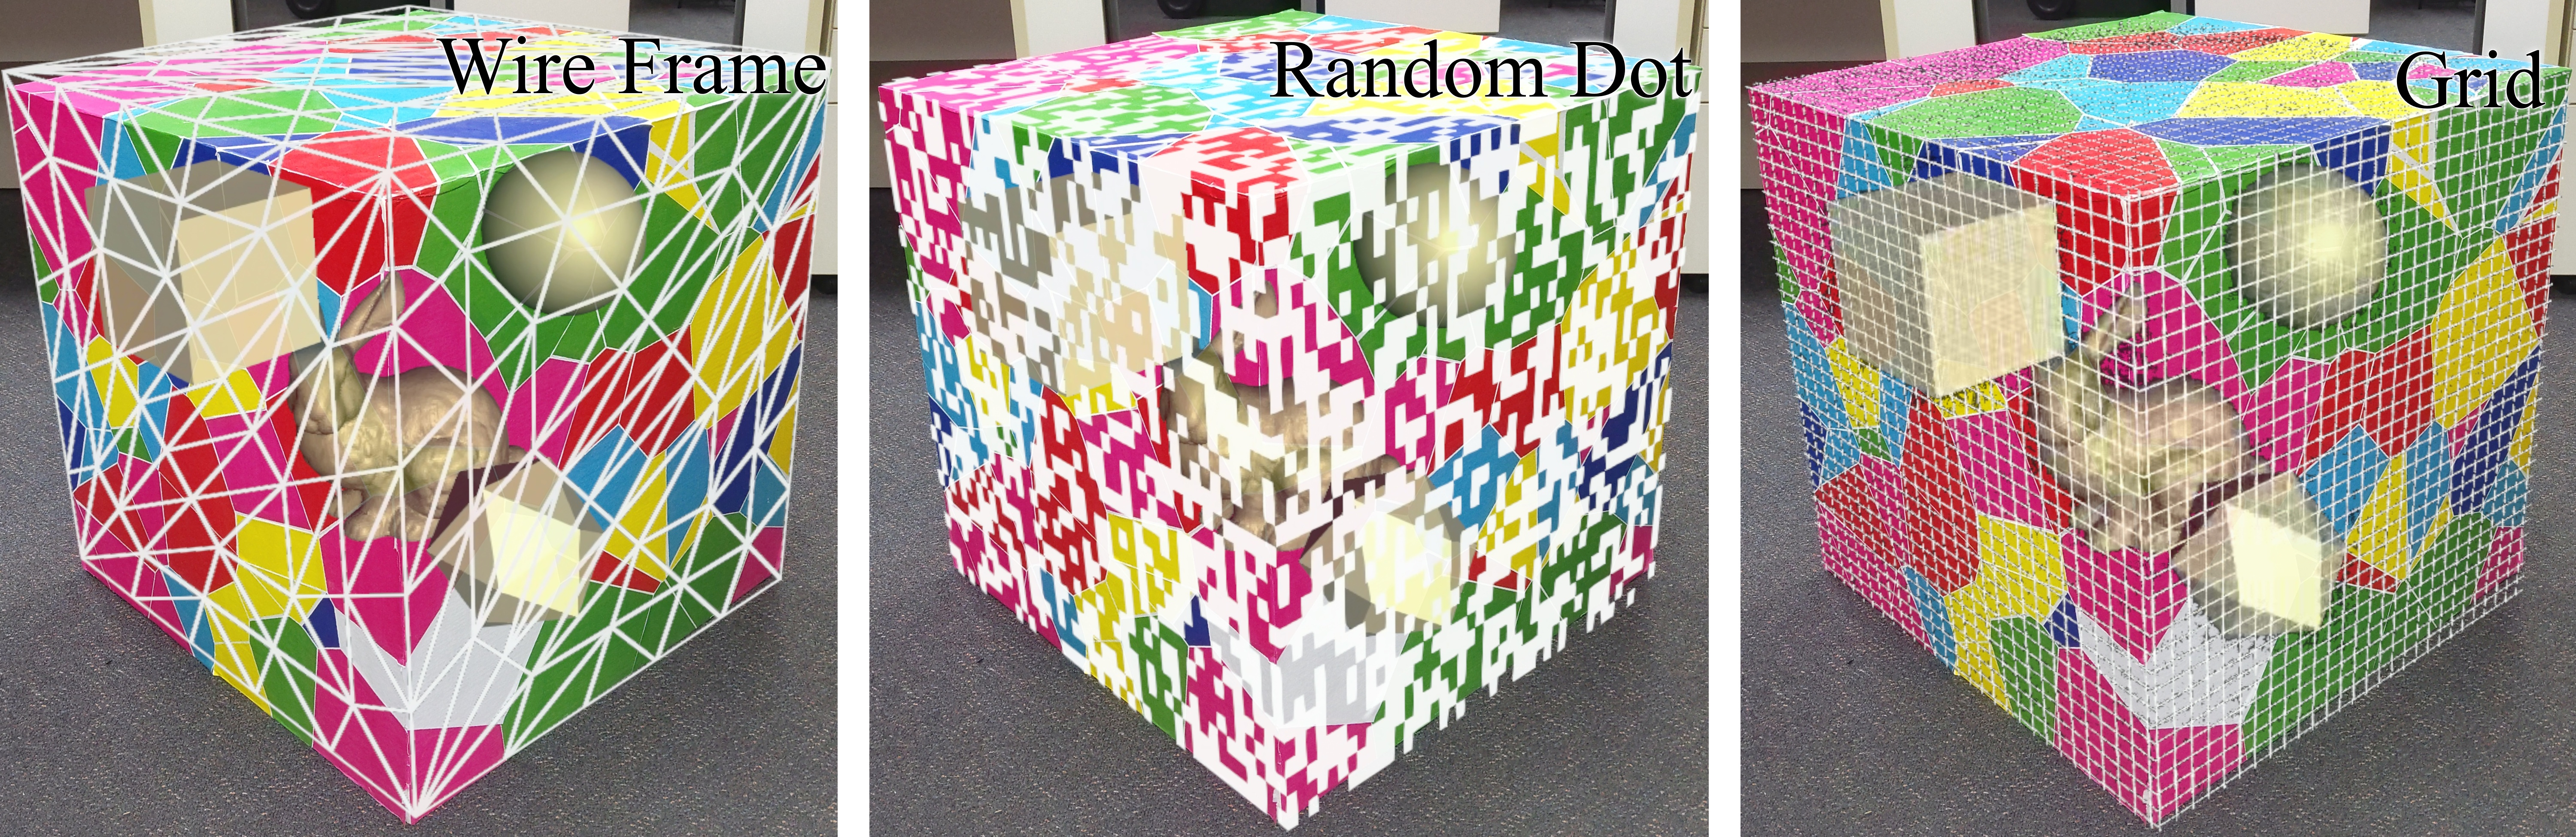
\includegraphics[width=\columnwidth]{Chapter2/Images/RealWorldOverlays.jpg}
    \caption[Wireframe, Random Dot, and Grid \gls{X-ray Visualization} over colorful patterned box with a virtual cube, sphere icosahedron, and a Stanford bunny rendered inside.]{This is a demonstration of real world overlay's and how they are utilized as forms of X-ray vision. the \glspl{X-ray Visualization} Wireframe, Random Dot, and Grid and are placed over colorful patterned box with a virtual cube, sphere icosahedron, and a Stanford bunny rendered inside. The image was taken using the HoloLens' screen view. }
    \label{fig:RealWorldOverlays}
\end{figure}

Overlaying a real-world overlay as a guide over the ground does not require any specific device since as long as the overlay is able to interact with the real world environment. 
It will perform better, however, when it is used with a binocular \gls{hmd} as this can better represent the surface~\cite{Otsuki2016}.
While they do provide a good occlusive cue, the main role they serve is to help the user locate the position of an object with reference to a real world object. 
The additional cues provided from that point moving forward should take note of what is required from that point moving forward. 

\autoref{fig:RealWorldOverlays} illustrates forms real-world overlays can take, for example overlaying grids~\cite{Becher2021, Heinrich2022, Heinrich2019, Johnson2014}, Wireframes~\cite{Chen2020, Gruenefeld2020, Tsuda2005} and Random Dots~\cite{Ghasemi2018, Otsuki2015, Otsuki2016, Otsuki2017}. All of these effects are designed to utilize partial occlusion to highlight the shape of the object and to help the user understand the orientation of the wall. This gives the user a better comprehension of the distance between themselves and the objects they are looking inside of. 

\paragraph{Grids:}
Grids allow for a persistent barrier between a given surface and provide a guide on where a surface is in an augmented world~\cite{Johnson2014, Heinrich2022}. 
Johnson et al.~\cite{Johnson2014} developed a surgical system that utilized a grid-based visualization to allow for \gls{ct} data to be viewed at the correct position within the patient when using a wearing an \gls{ar} \gls{hmd}.
A grid was utilized to represent different types of flesh and a 3D object. 
They had surgical students utilize this system with laparoscopic video to evaluate it, where it was received with a positive reception from the subjective study which was conducted~\cite{Johnson2014}. 

\begin{figure}
    \centering
    \includegraphics[width=\columnwidth]{Chapter2/Images/ImagesFromOtherWorks/Heinrich2022.png}
    \caption[The conditions utilized for Heinrich et al.'s~\cite{Heinrich2022}  research.]{The conditions utilized for Heinrich et al.'s~\cite{Heinrich2022} research. The first row shows how they were visualized using the HoloLens, while the second line shows the output from the \gls{sar} display. The columns represent the three visualizations they used in their study, which were then split into three, showing the difference between their visualizations for guiding the angle and depth required for the needle. Used with permission from IEEE \textcopyright{} 2022.}
    \label{fig:Heinrich2022}
\end{figure}

Grids also tend to be utilized to explain to the user where the background of the \gls{X-ray Visualization} can be seen. 
\autoref{fig:Heinrich2022} shows how Heinrich et al.~\cite{Heinrich2022} utilized a grid overlaying a virtual hole and tested how accurate a biopsy would be using this as visualizations between an \gls{ost} \gls{ar} and \gls{sar}. 
This required testing the accuracy of the initial insertion angle and the depth to which the user placed the device. 
Heinrich et al.~\cite{Heinrich2022} utilized two conditions without \gls{X-ray Visualization}. 
One was a target that showed and would change in color when the needle approached the target, and the other was a virtual needle for the users to match. 
%All the conditions are shown in \autoref{fig:Heinrich2022}.
%This method showed that the \gls{X-ray Visualization} was less effective than the glyph visualization, as the latter gave better feedback than being able to see the \gls{X-ray Visualization}. 
This method demonstrated that the glyph visualization was more effective than the \gls{X-ray Visualization}, as it provided participants with a more intuitive \gls{X-ray Vision} experiance.
However, both of them performed better than showing the visualization of the desired entry of the needle~\cite{Heinrich2022}. 

\paragraph{Random Dot:}
Random dot is another way of expressing more occlusion than other geometric pattern effects typically employed~\cite{Ghasemi2018, Otsuki2015}. This effect provides a partial sense of occlusion by providing a semi-occlusive layer over real-world objects~\cite{Otsuki2015}. 
This effect is one of the least computationally expensive but requires an immersive environment with flat surfaces. 
Highlighting various pixels on the surface of objects provides a stereoscopic effect of occlusion for the user and should technically allow for a better sense of depth. 

Ghasemi et al.~\cite{Ghasemi2018} conducted two studies to evaluate Random Dot visualizations. A psycho-physical depth perception experiment, which consisted of a series of thin circles, was run to determine the effectiveness of this \gls{X-ray Visualization}. 
Participants were given six different distances that ranged from 5mm in front and behind the visualization/wall.
The results study found that this effect is most effective when around 50\% of the space is filled using a random dot.
The amount of dots and their size could be altered, but it was most effective when more small dots were used up close and fewer larger ones up close and more remote. 
This distance could be increased if objects are further away from the wall, allowing for more depth perception. 

\paragraph{Halo and the Silhouette:}

% \begin{figure}[tb]
%     \centering
%     \includegraphics[width=0.75\columnwidth]{Chapter2/Images/JustHalo.png}
%     \caption{A directly rendered volume of a hierarchical set of spheres utilizing \gls{X-ray Visualization} that uses a silhouette/Halo \gls{X-ray Visualization}.}
%     \label{fig:JustHalo}
% \end{figure}
\begin{figure}[t]
    \centering
    \includegraphics[width=\linewidth]{Chapter2/Images/OzgurEtAl.png}
    \caption[Ozgur et al.'s~\cite{Ozgur2017} \gls{X-ray Vision} system using Halos.]{
    Ozgur et al.'s~\cite{Ozgur2017} \gls{X-ray Vision} system using Halos.
    The silhouettes are generated through orthographic projection onto the front and back planes, which are oriented based on the sight line passing through the tumor's center of mass. These planes are positioned at the points where the organ's surface intersects the sight line.
    Used with permission from IEEE \textcopyright{} 2017 and Ozgur et al.~\cite{Ozgur2017}
    }
    \label{fig:JustHalo}
\end{figure}

This effect goes by many names but is most commonly called Halo or Silhouette as it creates an outline of the virtual objects.
It will be referred to as the Halo visualization in this dissertation for simplicity.
The Halo \glspl{X-ray Visualization} as stated in Ozgur et al.'s~\cite{Ozgur2017} paper presents the effect as a bright light around the edges of the object of interest and use alpha blending to communicate depth~\cite{Ozgur2017}. 
%This is very similar to the silhouette effect found in medicine~\cite{Rheingans2001}, but since it is the only time this will be treated as if this is the termonlolgy for this effect in this thesis. 
This effect is very similar to what is referred to as the "silhouette" effect in medical visualization~\cite{Rheingans2001}. 
However, terminology varies across fields, and in this thesis, I will consistently use the term "Halo visualization" to describe this effect for clarity. 
\autoref{fig:JustHalo} show how the the halo is set to leverage the depth perception cue of relative size.
%In \autoref{fig:JustHalo}, it can be seen the halo's is set, allowing it to leverage the depth perception cue of relative size. 
This \gls{X-ray Vision} effect is unique due to its lack of occlusion, making it effective for surgical situations~\cite{Ozgur2017}. 
It has been tested using a monoscopic display in a study designed for minimally invasive surgeries. It can also exploit a color-based effect, applying visual language to communicate depth to the user~\cite{Ozgur2017}.

\subsubsection{Computer Vision-Enabled Techniques} \label{sec:ComputerVisionEnabledTechnqiue}
In computer vision, several methods are used to highlight salient features in an image. This is normally done by highlighting various salient factors within an image. 
These techniques are commonly used on monoscopic \gls{vst} devices as they provide a good sense of where an object is positioned relative to another in 2D. 
This is separate from the Halo technique as these do not generally utilize the image of the real world while the halo technique utilizes the shape of the object that has been inserted. 
To this date, the results lack the performance of Computer Vision-Enabled Techniques in stereo, with most of the publications found in this space either being demos or research proposals~\cite{Rompapas2014, Phillips2021}.

\begin{figure}[!b]
    \centering
    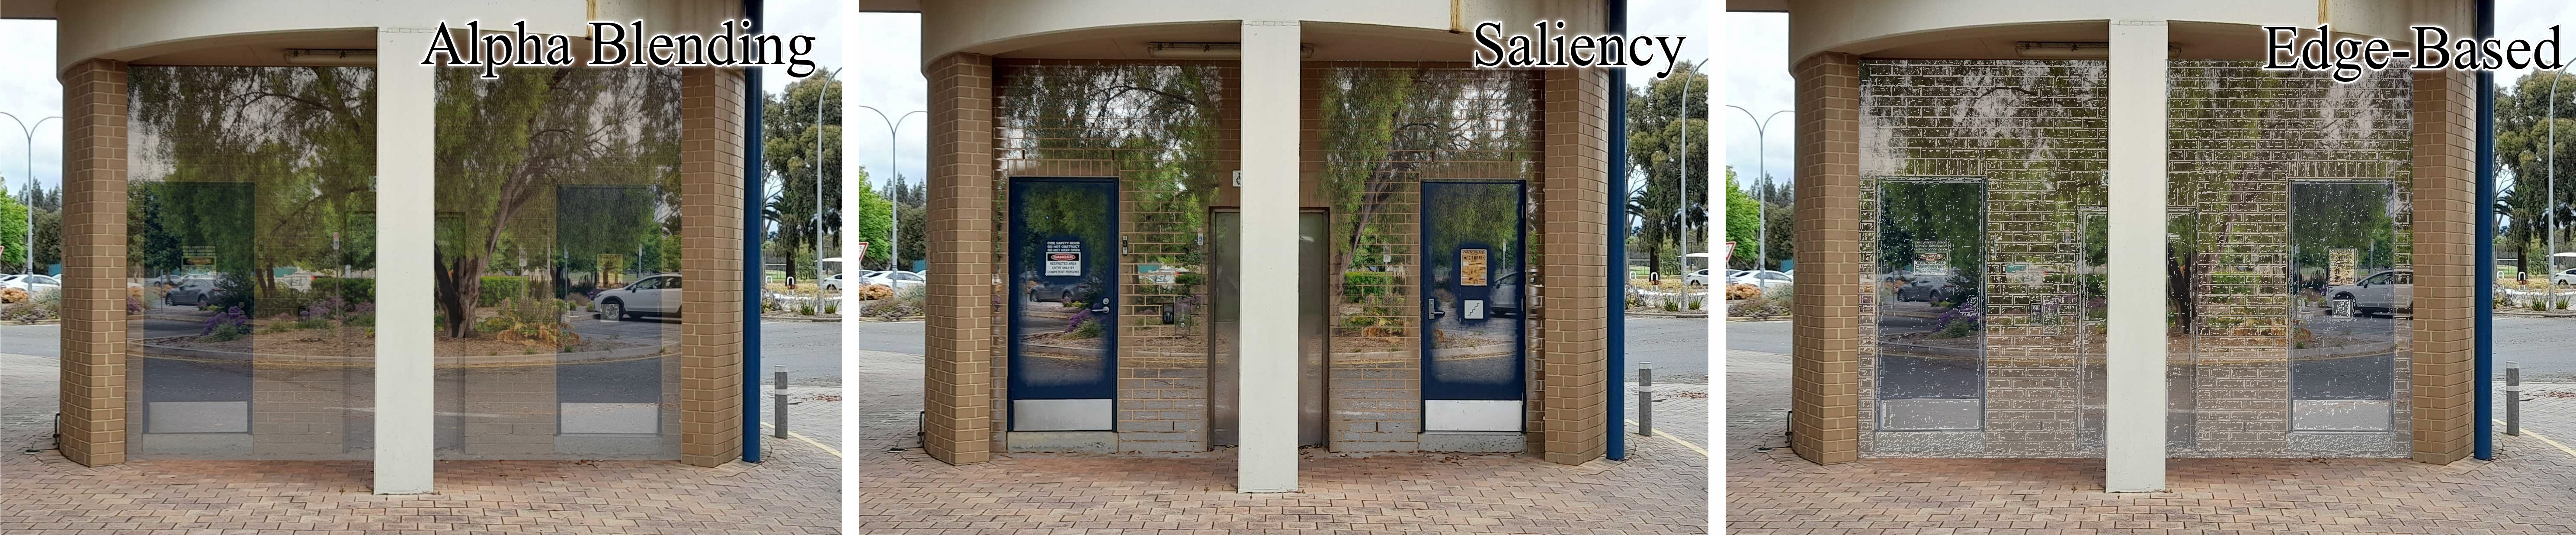
\includegraphics[width=\columnwidth]{Chapter2/Images/ComputerVisionEffectsAndTransperency.jpg}
    \caption{\gls{X-ray Vision} showing alpha blending, Saliency, and edge-based Visualizations (Shown left to right) looking through a building.}
    \label{fig:ComputerVisionEffectsAndTransperency}
\end{figure}

\paragraph{Edge-Based:}
Edge-based \glspl{X-ray Visualization} (depicted in \autoref{fig:ComputerVisionEffectsAndTransperency}) identify areas in the user’s view that contrast highly between neighboring pixels and highlight them. 
This high contrast effect tends to be regarded by most humans as salient, making it a reliable method for determining salient artifacts~\cite{Avery2009}. 
Created initially by Kalkofen et al.~\cite{Kalkofen2007} to allow for better image-based \gls{X-ray Vision}.
This visualization creates a predictable method for highlighting areas on an image (given that the surface has a high level of contrast) and makes it a popular way of showcasing \gls{X-ray Vision} on a monoscopic \gls{ar} device~\cite{Avery2009, Chen2010, Kalkofen2007, Sandor2010}. 
By highlighting the visible edges of an object, it is possible to create the appearance that an object is behind the object either through partial occlusion~\cite{Avery2009, Kalkofen2007} or by cutting out elements of the X-rayed object~\cite{Dey2012, Dey2014}.

\paragraph{Saliency:}
Saliency highlights areas of the real world that are likely to be of interest and makes the areas that are unlikely to be less apparent. 
\autoref{fig:ComputerVisionEffectsAndTransperency} shows one method of using saliency as an \gls{X-ray Visualization}. 
The visualization technique can vary between implementations because it can be done algorithmically~\cite{Sandor2010} or by training an AI model to detect the features a human is more or less likely to look at~\cite{Cong2019}. 
A user could naturally peer through objects using the saliency method, given that the camera could find some salient and non-salient areas of the image~\cite{Sandor2010}. 
As of the beginning of this thesis, Saliency has only been utilized with \gls{vst} \gls{ar}.

\paragraph{Ghosting:}
Ghosting utilizes the effects of visual saliency and focuses on allowing artistic approaches to partial occlusion~\cite{1238308, Zollmann2010}. Adaptive Ghosting is an extension that combines the salient effect of ghosting and edge-based \gls{X-ray Vision} effects. 

\begin{figure}[tb]
    \centering
    \includegraphics[width=1\linewidth]{Chapter2/Images/KalkofenEtAlSystem.png}
    \caption[A description of the \gls{X-ray Vision} system used by Kalkofen et al.~\cite{Kalkofen2013}]{A description of the \gls{X-ray Vision} system used by Kalkofen et al.~\cite{Kalkofen2013}. This image shows the various components of the graphics pipeline required to create the adaptive ghosting effect.
    (a) The occluder and occluded elements are combined into a ghosted view using state-of-the-art transparency mapping based on the importance map of the occluder. However, this initial ghosted view lacks is difficult to integrate into the real world seamlessly as it is either used to cover a area or it is not. To address this, a new importance map is generated for the resulting ghosted view which looks at area's of high contrast and places the visualisation on to them as well as over the rest of any are's close to virtual elements that need to be seen within the physical objects.
    (b) This new importance map is then compared to the original importance map of the occluder. Features that were marked as important in the occluder but are no longer prominent in the ghosted view are identified for enhancement.
    (c) By applying these enhancements to the adaptive ghosted view, the previously obscured important structures become clearly visible again.
    Used with permission from IEEE \textcopyright{} 2013.
    }
    \label{fig:KalkofenEtAlSystem}
\end{figure}

Zollman et al.~\cite{Zollmann2014} tested the effectiveness of Edge-Based, Ghosting, and Randomly occluding underground pipes.
Participants were asked to identify the depth of the pipes, which were located underground, based on a series of Images they received.
This study found that ghosting was better equipped than edge-based \gls{X-ray Vision} at identifying depth underground and noted that it was easy to use, but it did observe the details of the shape. 

Adaptive Ghosting technique to the current environment makes it less varied when viewing it from different directions~\cite{Kalkofen2013}.
\autoref{fig:KalkofenEtAlSystem} presents Kalkofen et al.'s~\cite{Kalkofen2013} system for Adaptive Ghosting, which normalizes the contrast of the input image to allow this effect to maintain a similar effect even in different lighting. 
This system combats one major issue with computer vision-enabled \gls{X-ray Vision} techniques: their inconsistency depending on changes to the scene and lighting. 
Adaptive Ghosting can cause unexpected artifacts and misleading visualizations, but it is still possible to notice this effect even when using Adaptive Ghosting.

\subsubsection{Comparisons Of X-ray Vision Effects}
% \begin{figure}[tb]
%     \centering
%     \caption{A heat map showing the frequency of pairwise comparison of different \gls{X-ray Vision} effects. The total number of studies for each effect is shown in the lower left to upper right diagonal.}
%     \label{fig:ComparisionsOFVisionInTheLiturature}
% \end{figure}

\begin{figure}[tb]
    \centering
    %\includegraphics[width=\columnwidth]{Chapter2/Images/ComparisionsOFVisionInThe Liturature.png}
    \includegraphics[width=\columnwidth]{Chapter2/Images/ComparisionsOFVisionInTheLiturature.pdf}
    \caption[A heat map illustrating how often different \gls{X-ray Vision} effects are compared to each other in the literature.]{
        A heat map illustrating how often different \gls{X-ray Vision} effects are compared to each other in the literature. The diagonal cells (from lower left to upper right) show the total number of studies for each effect, while the center row indicates studies that examined each effect individually without comparison.

        % A heat map showing the frequency of pairwise comparison of different \gls{X-ray Vision} effects found throughout the literature. The total number of studies for each effect is shown in the lower left to upper right diagonal. the center row is focused on the number of studies that did not compare the effect to another.
        }
    \label{fig:ComparisionsOFVisionInTheLiturature}
\end{figure}

Given all these methods of \gls{X-ray Vision}, it is quite common for people to try to compare them to determine the positive and negative aspects. 
Studies in this area have investigated:
\begin{itemize}
    \item The amount of occlusion density required for visualizations to create the \gls{X-ray Vision} visualisations and effective limits to the practicality of these effects~\cite{Santos2016};
    \item How different displays react to \glspl{X-ray Visualization} on Mobile Devices~\cite{Dey2012, Dey2014}.
    \item What is the impact of \gls{X-ray Vision} between different visualizations~\cite{Sandor2010, Zollmann2014, Martin-Gomez2021, Gruenefeld2020}.
\end{itemize}
These comparisons are detailed in \autoref{fig:ComparisionsOFVisionInTheLiturature}.

Partial occlusion is important to most \glspl{X-ray Visualization}. It shows how much occlusion is needed for a given technique and how much occlusion makes interactions impossible.
This was the question that Santos et al.~\cite{Santos2016} addressed for mobile \gls{ar} \gls{X-ray Vision} when using edge-based or saliency \gls{X-ray Vision} effects.
This study had participants look at a box wrapped in either wrapping paper or crumpled foil.
This study utilized two tasks: One looking at what thresholds were required to allow participants to see 2D objects using \gls{X-ray Vision} effects, and the other looking at the maximum allowable alpha values these effects could have~\cite{Santos2016}. 

Santos et al.'s~\cite{Santos2016} first tested how the user could see four objects placed inside the box and asked them to reveal the maximum decision cutoff (threshold).
The next task was to lower the alpha value of the visualization until participants could clearly see the object hidden behind it. 
Inside the box would be visualized an image of an object they were asked to see, which could either be a small or a large object about the box. 
Each second, the transparency of the visualization would decrease, asking them to press a button on the display to stop the visualization when they could identify the item.
The combination of Santos et al.'s~\cite{Santos2016} results indicates the clarity of the object was dependent on the size, color, and texture of the box rather than the visualization used. 
The study noted Saliency was slightly harder to see through but not to a significant level. 
This dissertation treats these results as a guideline and has based its use of transparency and contrast with \gls{X-ray Vision} on these results. 

Sandor et al.~\cite{Sandor2010} Compared Edge-based visualizations to their newer Saliency visualization by having participants try to find a target in four scenes. 
This study found little difference between saliency and edge-based visualizations, but participants preferred the edge overlay. 
After this, both these conditions were tested using an online survey where participants would look at images presenting the information where saliency was seen to be better for providing \gls{X-ray Vision} for images. 

Dey et al.~\cite{Dey2012, Dey2014} compared \gls{X-ray Vision} on different-sized mobile devices to determine the display size could impact the visualizations required for Mobile devices.
Firstly, they developed an \gls{X-ray Visualization} called Melt, which showed a part of the foreground and a part of the background together.
Their first experiment tested the Edge-based technique against the Melt X-ray technique from far distances using a 7-inch display.
This study found that Melt was a more accurate in-depth estimation but took the participants longer to judge, which was likely used to overcome the drawbacks of the visualization~\cite{Dey2012, Dey2014}.

Dey et al.~\cite{Dey2014} ran a user study comparing Edge-based and Saliency using a Mobile \gls{ar} display. 
They created three levels of each \gls{X-ray Visualization}, where they were more or less sensitive to environmental concerns.
These results indicated that users struggled to use \gls{X-ray Visualization} when the edges were too thick for the edge-based variable, and saliency struggled in bright environments. 

All of the comparisons explained in this section utilized similar \gls{X-ray Vision} visualizations and most focused on how \glspl{X-ray Visualization} worked in different areas.
All these examples utilize mobile devices, so how these would affect \glspl{hmd} in general is a question that is yet to be answered. 
Also, most of these comparisons have utilized various forms of computer vision techniques (except for one use of the Melt visualization). 
Currently, there are many unknowns that exist in this space.


\subsection{Applications of X-ray Vision}

\begin{figure}[tb]
    \centering
    \includegraphics[width=\columnwidth]{Chapter2/Images/ImagesFromOtherWorks/Eren2018.png}
    \caption[Eren et al.'s~\cite{Eren2013} different visualizations of underground pipe networks using \gls{X-ray Vision} techniques.]{Eren et al.'s~\cite{Eren2013} different visualizations of underground pipe networks using \gls{X-ray Vision} techniques. a) baseline, b) edge-based, c) virtual hole, and d) cross-sectional techniques. Used with permission from Springer Nature \textcopyright{} 2018.}
    \label{fig:Eren2013}
\end{figure}

X-ray vision has been applied across a wide range of domains where visualizing hidden or internal structures is valuable. Medical research has been a central focus, where overlays of anatomical structures can support diagnosis and guide surgical procedures by allowing clinicians to perceive organs, tissues, and bones in situ~\cite{Bichlmeier2007, Blum2012, Bajura1992}. While demonstrations have shown promise, challenges remain around depth perception and real-time performance, as highlighted in comparative evaluations of iso-surfaces, direct volume rendering, and alternative rendering effects~\cite{Sielhorst2006, Bichlmeier2007}. Outside of medicine, construction and maintenance tasks also benefit, with researchers exploring techniques for seeing into walls or underground pipe networks. Early work by Feiner et al.~\cite{Feiner1995} focused on gradually revealing occluded structures, and more recent studies (e.g., Eren et al.~\cite{Eren2013,Eren2018}, shown in \autoref{fig:Eren2013}) have evaluated different visualization methods for accurately perceiving underground utilities.

Beyond these domains, X-ray vision concepts have been investigated in security, navigation, and education. In security, transparency effects and perspective-corrected projections have been used to augment situational awareness, though evaluations suggest togglable, more occlusive effects may be most effective~\cite{Kameda2004, Tsuda2005, Ohta2010}. Navigation and tourism applications demonstrate how seeing through structures or into the past can improve wayfinding and enrich cultural experiences, with evaluations showing reduced cognitive load compared to traditional maps~\cite{Dey2011, Maia2016, Yamamoto2014}. In education, while the effects of X-ray vision itself remain underexplored, augmented reality has been shown to increase engagement and may support long-term retention in domains like anatomy~\cite{Akpan2019, Santos2015}.

Entertainment provides a final but growing space for X-ray vision. While formal research is limited~\cite{Guo2023}, several commercial AR games such as Microsoft’s RoboRaid and Dr. Grordborts Invaders (shown in \autoref{fig:DrGrordbortsInvaders}) have experimented with the concept, using it to merge real and virtual environments in playful, interactive ways. These applications highlight both the versatility of X-ray vision across domains and the ongoing challenges of designing visualization techniques that are perceptually effective, intuitive, and computationally feasible.

\begin{figure}[tb]
    \centering
    \includegraphics[width=\columnwidth]{Chapter2/Images/ImagesFromOtherWorks/DrGrordbortsInvaders.jpg}
    \caption[A promotional Image from Dr Grordborts Invaders made by Weta Workshop for the Magic Leap.]{A promotional Image from Dr Grordborts Invaders made by Weta Workshop for the Magic Leap. Used with permission from Weta Workshop.}
    \label{fig:DrGrordbortsInvaders}
\end{figure}


\subsection{Hardware For X-ray Vision}
\glspl{X-ray Visualization} can be split into two key components to enable \gls{X-ray Vision}: A display to view the visualization and sensors to collect the data for \gls{X-ray Vision}.
While many studies have utilized collected information, allowing them to require only devices to collect pre-rendered devices, others have utilized a display. 
%Even then, \gls{X-ray Vision}, the type of \gls{X-ray Vision} used, tends to be influenced by the display utilized.

\glspl{X-ray Visualization} rely on two essential aspects: the availability of data representing the internal or hidden structures, and the means to visualize this data effectively. While many studies utilize pre-existing or independently collected datasets, others focus on the development and evaluation of display technologies for presenting \gls{X-ray Vision}. It is important to note that data acquisition is typically a separate process from visualization, and in most cases, data is gathered without a specific visualization method in mind.
However, the choice of data acquisition can limit the types of visualizations that can be effectively employed. For instance, real-time data acquisition methods may restrict the complexity of visualizations due to processing constraints, while pre-collected datasets allow for more intricate and computationally intensive visualization techniques.

\begin{figure}[tb]
    \centering
    \includegraphics[width=\columnwidth]{Chapter2/Images/DispalyModesUsedForXRayVis.png}
    \caption{A bar graph of the type of display used to visualize the various \gls{X-ray Vision} effects.}
    \label{fig:DispalyModesUsedForXRayVis}
\end{figure}

\subsubsection{Displays}
% \gls{X-ray Vision} is possible on any augmented reality device, ranging from phones to head-mounted displays, but can also extend to systems of static screens in the real world that react to gesture-like commands~\cite{Park2021}. 
% In this field, many different displays have been used to create different display technologies from varying perspectives and display types. 
\gls{ar} displays come in different variations, each with its own benefits.
These different types of displays can be generalized as \gls{ost} \gls{ar}, \gls{vst} \gls{ar}, and \gls{sar}.
\gls{ost} \gls{ar} works by projecting the image on a transparent reflective display, creating a transparent display which is generally used for \glspl{hmd}.
\gls{vst} \gls{ar} displays utilize one or more cameras and display them with graphics overlaid on them. 
\gls{sar} uses projectors to place computer graphics to overlaid onto reality.
\autoref{fig:DispalyModesUsedForXRayVis} shows there are preferences between different types of \gls{X-ray Vision} devices to an extent due to the individual benefits and drawbacks caused by these displays which have been laid out in \autoref{tab:XRayVisionDeviceComparison}.
\autoref{fig:ARTypesAndVisUsage}, shows real-world overlays are much more common than computer vision techniques, but real-world visual techniques are less common on monoscopic displays. 



% Define a compact list environment for tight bullet spacing
% Define compact list environment with sublist support
\newlist{titemize}{itemize}{3}
% Level 1 (top level)
\setlist[titemize,1]{label=--, left=0pt, itemsep=1pt, topsep=2pt, parsep=0pt}
% Level 2 (sublists)
\setlist[titemize,2]{label=$\ast$, left=1.5em, itemsep=1pt, topsep=1pt, parsep=0pt}
% Level 3 (sub-sublists, optional)
\setlist[titemize,3]{label=$\circ$, left=3em, itemsep=1pt, topsep=1pt, parsep=0pt}


\begin{table}[ht]
    \small
    \centering
    \caption{Advantages and Disadvantages of Devices Used for X-ray Vision}
    \label{tab:XRayVisionDeviceComparison}

    %%%%%%%%%%%%%%%%%%%%%%
    % Device 1
    %%%%%%%%%%%%%%%%%%%%%%
    \begin{tabular}{p{0.45\linewidth}|p{0.45\linewidth}}
        \hline
        \multicolumn{2}{c}{\textbf{OST AR Head-Mounted Displays (Optical See-Through)}} \\
        \hline
        \textbf{Advantages} & \textbf{Disadvantages} \\
        \hline
        \begin{titemize}
            \item Direct view of real world with overlays
            \item Maintains natural depth cues and peripheral vision
            \item Good for tasks needing situational awareness (e.g., surgery)
            \item Hands-free operation
        \end{titemize}
        &
        \begin{titemize}
            \item Limited brightness and contrast
            \item Smaller field of view vs. VST
            \item Alignment/calibration issues
            \item Optical distortion of virtual content
            \item Lower graphical fidelity
        \end{titemize} \\
    \end{tabular}
    \vspace{1em}

    %%%%%%%%%%%%%%%%%%%%%%
    % Device 2
    %%%%%%%%%%%%%%%%%%%%%%
    \begin{tabular}{p{0.45\linewidth}|p{0.45\linewidth}}
        \hline
        \multicolumn{2}{c}{\textbf{VST AR Head-Mounted Displays (Video See-Through)}} \\
        \hline
        \textbf{Advantages} & \textbf{Disadvantages} \\
        \hline
        \begin{titemize}
            \item High graphical fidelity and brightness
            \item Easier integration of computer vision
            \item Wider field of view possible
            \item Flexible virtual content manipulation
        \end{titemize}
        &
        \begin{titemize}
            \item Camera-mediated view
            \begin{titemize}
                \item Latency
                \item Distortion
            \end{titemize}
            \item Lower situational awareness
            \item Reduced situational awareness
            \item Can cause motion sickness
            \item Heavier, bulkier hardware
        \end{titemize} \\
    \end{tabular}
    \vspace{1em}

    %%%%%%%%%%%%%%%%%%%%%%
    % Device 3
    %%%%%%%%%%%%%%%%%%%%%%
    \begin{tabular}{p{0.45\linewidth}|p{0.45\linewidth}}
        \hline
        \multicolumn{2}{c}{\textbf{Mobile Devices (Phones/Tablets)}} \\
        \hline
        \textbf{Advantages} & \textbf{Disadvantages} \\
        \hline
        \begin{titemize}
            \item Widely available, easy to use
            \item Bright displays
            \item Portable for quick tasks
            \item Stable, high-quality graphics
        \end{titemize}
        &
        \begin{titemize}
            \item Less immersive
            \item Must be handheld
            \item Smaller screens limit detail
            \item Hardware fragmentation
            \item Limited spatial interaction
        \end{titemize} \\
    \end{tabular}
    \vspace{1em}

    %%%%%%%%%%%%%%%%%%%%%%
    % Device 4
    %%%%%%%%%%%%%%%%%%%%%%
    \begin{tabular}{p{0.45\linewidth}|p{0.45\linewidth}}
        \hline
        \multicolumn{2}{c}{\textbf{Spatial Augmented Reality (SAR) / Projectors}} \\
        \hline
        \textbf{Advantages} & \textbf{Disadvantages} \\
        \hline
        \begin{titemize}
            \item Projects info directly on objects
            \item Multiple users at once
            \item No wearables needed
            \item Limited multi-user suitability
        \end{titemize}
        &
        \begin{titemize}
            \item Needs precise calibration/tracking
            \item Works best in controlled environments
            \item Sensitive to lighting/surface
            \item Limited multi-user suitability
        \end{titemize} \\
    \end{tabular}
    \vspace{1em}

    %%%%%%%%%%%%%%%%%%%%%%
    % Device 5
    %%%%%%%%%%%%%%%%%%%%%%
    \begin{tabular}{p{0.45\linewidth}|p{0.45\linewidth}}
        \hline
        \multicolumn{2}{c}{\textbf{Desktop/Fixed Screens}} \\
        \hline
        \textbf{Advantages} & \textbf{Disadvantages} \\
        \hline
        \begin{titemize}
            \item High computational power
            \item Stable, high-quality graphics
            \item Large display for detail
            \item Comfortable for long use
            \item Good for collaboration
            \item Easy integration with systems
        \end{titemize}
        &
        \begin{titemize}
            \item Not immersive
            \item Stationary, low spatial interaction
            \item Requires looking away from real world
            \item Limited field of view
            \item Not mobile-friendly
        \end{titemize} \\
    \end{tabular}

\end{table}

\renewlist{titemize}{itemize}{1}
\setlist[titemize,1]{}


% \begin{table}[ht]
%     \centering
%     \caption{A table describing the Advantages and Disadvantages of Devices Used for X-ray Vision}
%     \begin{tabular}{l|l}
%         \hline
%         \textbf{Device Type} & \textbf{Advantages} & \textbf{Disadvantages} \\
%         \hline
%         OST AR Head-Mounted Displays (Optical See-Through) &
%         \begin{itemize}
%             \item Allows direct view of the real world with virtual overlays
%             \item Maintains natural depth cues and peripheral vision
%             \item Suitable for tasks requiring high situational awareness (e.g., surgery)
%             \item Hands-free operation
%         \end{itemize} &
%         \begin{itemize}
%             \item Limited brightness and contrast of virtual content
%             \item Smaller field of view of virtual objects compared to VST
%             \item Alignment/calibration issues can affect accuracy
%             \item Distortion of virtual content due to optics
%             \item Lower graphical fidelity due to transparent displays
%         \end{itemize} \\
%         \hline
%         VST AR Head-Mounted Displays (Video See-Through) &
%         \begin{itemize}
%             \item High graphical fidelity and brightness
%             \item Easier to integrate advanced computer vision techniques
%             \item Can provide a wider field of view
%             \item More flexible for virtual content manipulation
%         \end{itemize} &
%         \begin{itemize}
%             \item Real-world view is mediated by cameras (can introduce latency and distortion)
%             \item Reduced situational awareness and peripheral vision
%             \item Potential for motion sickness or discomfort
%             \item Heavier and bulkier hardware
%         \end{itemize} \\
%         \hline
%         Mobile Devices (Phones/Tablets) &
%         \begin{itemize}
%             \item Widely available and easy to use
%             \item Bright displays, good visibility
%             \item Portable for quick tasks
%             \item Stable, high-quality graphics
%         \end{itemize} &
%         \begin{itemize}
%             \item Less immersive
%             \item Must be held by user
%             \item Smaller screens limit detail
%             \item Too many different hardware specifications
%             \item Limited spatial interaction
%         \end{itemize} \\
%         \hline
%         Spatial Augmented Reality (SAR) / Projectors &
%         \begin{itemize}
%             \item Overlays info directly onto physical objects
%             \item Multiple users can view simultaneously
%             \item No wearable device needed
%         \end{itemize} &
%         \begin{itemize}
%             \item Requires precise calibration/tracking
%             \item Best in controlled environments
%             \item Limited by lighting and surface properties
%             \item Not suitable for multiple users.
%         \end{itemize} \\
%         \hline
%         Desktop/Fixed Screens &
%         \begin{itemize}
%             \item Allows for high computational power
%             \item Stable, high-quality graphics
%             \item Large display area for detail
%             \item Comfortable for long-term use
%             \item Good for collaborative tasks
%             \item Easily integrated with existing systems
%         \end{itemize} &
%         \begin{itemize}
%             \item Not immersive
%             \item Stationary, limited spatial interaction
%             \item Requires user to look away from real world
%             \item Limited field of view for spatial tasks
%             \item Not suitable for mobile tasks
%         \end{itemize} \\
%         \hline
%     \end{tabular}
%     \label{tab:XRayVisionDeviceComparison}
% \end{table}

\gls{X-ray Vision} systems can be supported by display devices, including mobile phones, head-mounted displays, computer screens, and projectors~\cite{Kim2018}. Devices range from traditional computer screens and mobile personal devices, head-mounted displays to projectors. 
Most earlier devices only accommodate monocular vision, while recent head-mounted displays can support stereoscopic vision. \autoref{fig:LitRevewDeviceFrequencyPlot} shows that the choice of technology is often a result of technological advances and emerging products. It can be observed that mobile screen-based displays were most popular following the release of powerful mobile phones in 2007, underpinned by emerging computer vision techniques for tracking and the generation of visualizations. Similarly, stereoscopic head-mounted displays have gained popularity because of increased capabilities, technology maturity, and general availability in recent years.

Recently, research utilizing Microsoft HoloLens 1 and 2 has been widely used in \gls{X-ray Vision} research because of their advanced display tech and gesture recognition, making them a useful device for security and medical operations~\cite{Phillips2020, Martin-Gomez2021, Rodrigues2017, AlJanabi2020}. \glspl{hmd} shine in medical settings, offering a sterile work environment. Medical applications use screens for remote interactions, like controlling robotic arms in minimally invasive surgery~\cite{Kalia2019}. In contrast, the construction and maintenance industries employ diverse devices due to their varied environments~\cite{Muthalif2022, Eren2013, Eren2018, Becher2021}.

\begin{figure}[bt]
    \centering
    \includegraphics[width=\columnwidth]{Chapter2/Images/ARTypesAndVisUsage.png}
    \caption{A bar graph displaying The types of \gls{ar} that was used to visualize the different types of \gls{X-ray Vision} effects.}
    \label{fig:ARTypesAndVisUsage}
\end{figure}


%%% Toms notes I revised this section to remove some of the repetition and make it clearer.
% Some froms of AR do not require wearable devices at all. Spatial Augmented Reality (\gls{sar}) uses projectors to overlay digital content onto physical objects and surfaces in the real world.
% %Creating an immersive experience without the need for head-mounted displays or handheld devices.
% \autoref{fig:LitRevewDeviceFrequencyPlot} shows SAR techniques are a relatively novel addition to \gls{X-ray Vision}, where only a few papers have been published however, they are one of the few area's of x-ray vision that has been adopted by industry Augmetrics~\footnote{\url{https://augmedics.com/}} has created a system that utilizes \gls{sar} to project medical insuctions onto a patient's body, allowing surgical staff to gain insight into the body without looking away from the patient.
% Both \autoref{fig:DispalyModesUsedForXRayVis} and \autoref{fig:ARTypesAndVisUsage} show the flexibility of \gls{sar} displays tend to be very flexible, allowing and possess both the ability to utilize Real real-world overlays, computer enabled techniques and visualization effects. 
% In contrast to head-mounted or fixed display devices, \gls{sar} technologies can augment the physical environment in situ without obstructing the user’s field of view~\cite{Heinrich2019, Heinrich2019b}. However, accurate calibration and tracking of the user’s vantage point are essential for high-precision \gls{X-ray Vision}. 
% Generally, \gls{X-ray Vision} SAR-based systems are uncommon but have been done in medical settings and settings where the user is relatively stationary and needs an unobscured vision~\cite{Heinrich2019}.

\subsubsection{Comparison of Displays} \label{sec:ComparisionOfDisplays}
Comparing the effectiveness of different displays seems to be a relatively new area of study for \gls{ar} enabled \gls{X-ray Vision}.
Prior to starting this dissertation in 2019, our review found no studies that compared \glspl{X-ray Visualization} between different papers.
Since then, several studies have published their results on comparing \gls{vst} \gls{ar} devices against \gls{ost} \gls{ar} devices.

Gruenefeld et al.~\cite{Gruenefeld2020} performed depth perception studies using an OST headset utilizing \gls{X-ray Vision}, including Grid, Cut-out effects. 
The grid effect, placed on the ground within the X-ray able space and a perpendicular wall facing the viewer, could be used to approximate a relationship between the wall and the object. In contrast, the cut-out visualization provided a hole in the wall, which the user could look through to see where the object was on the other side, against a baseline that pointed participants to the object with a red arrow and displayed a perpendicular line going from the far point of the arrow to the bottom of the visualization. 
Gruenefeld et al.'s~\cite{Gruenefeld2020} found that the weakest of the depth cues were the cut-out. This was because the cues did not convey a clear depth indications to the user~\cite{Gruenefeld2020}, because the grid effect provided a clear indication of depth, allowing the users to count the amount of grid squares between the object and the wall they had a better sense of depth.

Another set of studies published by Martin-Gomez et al.~\cite{MartinGomez2021} studied the difference between four \glspl{X-ray Visualization} (None (Superimposition), virtual hole, ghosting, and Random Dot) on both \gls{vst} \gls{ar} and \gls{ost} \gls{ar} devices in the near field. 
They found that users better utilized \gls{X-ray Vision} on a \gls{vst} \gls{ar} headset than on an \gls{ost} \gls{ar} device.
This prompted another study investigating different rendering techniques for \gls{X-ray Vision} (shading, hatching, ghosting) and brightness levels, finding that bright, clear objects work best in \gls{ost} \gls{ar}.

Heinrich et al.'s~\cite{Heinrich2022} research comparing \gls{ost} \gls{ar} displays to \gls{sar} displays (previously mentioned in \autoref{sec:realWorldOverlay}) presented findings that both \gls{ost} \gls{ar} and \gls{sar} displays functioned in a similar fashion. 
%However, they did find that \gls{X-ray Vision} works better with \gls{ost} \gls{ar} displays while \gls{ui} elements (\autoref{fig:Heinrich2022} Glyph Vis) tend to function better when using projectors.
However, they found that \gls{X-ray Vision} works better with \gls{ost} \gls{ar} displays, while \gls{ui} elements (see \autoref{fig:Heinrich2022}, Glyph Vis) tend to function better when using projectors.
These different conditions can be seen and compared in \autoref{fig:Heinrich2022}.
%The details of this research were previously mentioned in \label{sec:realWorldOverlay}.

\begin{figure}
    \centering
    \includegraphics[width=\columnwidth]{Chapter2/Images/LitRevewDeviceFrequencyPlotBar.pdf}
    \caption[Devices examined for X-ray vision across the literature over time.]{Devices examined for X-ray vision across the literature over time. Each point represents a publication, categorized by device type (vertical axis) and year of appearance (horizontal axis). The distribution highlights how research interest has shifted across different device categories, with increased attention to head-mounted displays and mobile devices in more recent years.}
    \label{fig:LitRevewDeviceFrequencyPlot}
\end{figure}

\subsubsection{Sensors Utilized}

%An IoT metaverse is created by a collection of sensors located in various devices and around the user's environment, if not the entire world~\cite{Asif2023, } (Asif and Hassan 2003; Blanco-Novoa et al. 2020). Not only do these devices need to be calibrated to work together, but they also need to be able to visualize a world connected that is comprehendible to its users (Pereira et al. 2019). None of the literature used this as a whole, but several different techniques have been created to visualize \gls{X-ray Vision}. 

The information used in \gls{X-ray Vision} applications may possess different characteristics, such as the nature of the data, its temporal characteristics, and its realism. Three-dimensional models, point clouds, video feeds and photos, medical data, and depth maps are examples of the diversity of data visualized in \gls{X-ray Vision}. Moreover, one can distinguish static information, which remains unchanged for a task, from dynamic information, which may change during a task. Finally, the degree of realism of the data can vary. 

\autoref{fig:LitReviewDevicesBeingUsed} illustrates that static information prevails as the most common virtual element in \gls{X-ray Vision}, constituting 65\% of the 54 papers examined. Examples include 3D models, medical images, and building schematics, predominantly found in medical, construction, and maintenance domains. Virtual objects range from simple geometric shapes to intricate representations of real objects~\cite{Becher2021, Eren2013, Eren2018, Muthalif2022, Zollmann2014}.

% Dynamic data, as depicted in \autoref{fig:LitReviewDevicesBeingUsed}, often comprises video feeds from static or mobile cameras. This technique, capturing information from multiple perspectives, enables users to perceive distant or hidden details while viewing the actual environment simultaneously. Security and robotic system control applications benefit from these methods~\cite{Erat2018, Phillips2021}. The real-time delivery of camera-captured information mirrors the real world, with non-dynamic data commonly used in construction to model underground pipes. This addresses the challenge of communicating the position of underground structures to end users~\cite{Becher2021, Eren2018, Eren2013, Muthalif2022, Zollmann2014}. Notably, \gls{X-ray Vision} experiments in construction consistently utilize simulated data, aiming to replicate real-world scenarios.

Dynamic data, as shown in \autoref{fig:LitReviewDevicesBeingUsed}, typically consists of video feeds from static or mobile cameras. By providing multiple perspectives in real time, these feeds allow users to perceive distant or hidden details while still observing the actual environment, a capability that has proven valuable in domains such as security and robotic system control~\cite{Erat2018, Phillips2021}. In contrast, non-dynamic data is often employed in construction, where pre-recorded or modelled information is used to represent underground pipes and other hidden infrastructure~\cite{Becher2021, Eren2018, Eren2013, Muthalif2022, Zollmann2014}. Within this context, \gls{X-ray Vision} studies in construction have relied primarily on simulated data to approximate real-world conditions and to address the challenge of clearly communicating the location of underground structures to end users.

Most of the research that utilizes live recordings in this review employed cameras or medical equipment (shown in \autoref{fig:LitReviewDevicesBeingUsed}). No studies were found that visualized radar and other sensor data in a 3D manner to create an \gls{X-ray Vision} effect—limiting the types of visualizations that people were viewing. Techniques like photogrammetry were not found either which would be able to recreate images from several views into a 3D scene~\cite{Nguyen2013, Pereira2019}. This suggests that, so far, \gls{X-ray Vision} has primarily focused on presenting users with visualizations of the known world. In contrast, little work has explored systems that could reveal entirely unknown or hidden environments in real time, effectively giving users access to true X-ray vision.

\begin{figure}
    \centering
    \includegraphics[width=\columnwidth]{Chapter2/Images/LitReviewDevicesBeingUsed.png}
    \caption[A plot showing nine devices found in the literature.]{A plot showing nine devices found in the literature. Head-mounted displays used as display devices are grouped. Portable screens like phones and tablets, larger screens, and magic mirrors fall under the 'Screens' category. Additionally, three user studies utilized Images and \gls{sar}.}
    \label{fig:LitReviewDevicesBeingUsed}
\end{figure}


% An explanation of Augmented Reality
\section{Perception and Depth Perception tasks in Augmented Reality (AR) and Virtual Reality (VR) Head Mounted Displays}
% This section is talking about the issues of depth perception in oST AR
% The ability to modify our visual perception of the world allowed for an almost limitless amount of possibilities of changes that are possible to augment people's vision. 
% However, this required us to learn about the limitations of this perception beyond what we could see naturally. 
% The most major form of this was to gain a concrete understanding of how depth worked when displaying a 2D image. 
% The visual impacts that have been caused by these devices were caused by the camera lenses don't see the world the same way as people do, so the displays would need to appear~\cite{Cutting1997}.

Depth perception on \gls{mr} \glspl{hmd} has been a goal for over 25 years~\cite{Cutting1997}.
%\gls{mr} \glspl{hmd} tend to be quite limited in methods that are possible to use to measure how a participant can measure depth in the real world, which has prompted 
Several common methods of testing depth perception in the real world. These include 
\begin{itemize}
    \item \textbf{Blind Walking or Blind reaching:} Asking a participant to place their hands or to walk to a location where a virtual artifact was previously~\cite{Jamiy2019, Jamiy2019b};
    \item \textbf{Verbal Reporting:} Requesting the participant tell you how far away the virtual object is from them~\cite{Jamiy2019, Jamiy2019b};
    \item \textbf{Matching Protocols: } Placing a virtual object relive to where the virtual object is (or was)~\cite{Jamiy2019, Jamiy2019b};
    \item \textbf{\gls{twofc_g}:} Giving the participant where there is one correct and wrong answer on a set of conditions that will get closer to being equal to determine at what point can participants no longer determine proper depth perception~\cite{Otsuki2017, Fan1996}.
\end{itemize}
%Using these types of studies 
% Start talking about the early work trying to understand depth in AR and VR
%early work in this field focused on testing how seeing graphics rendered using virtual reality headsets may have changed. 
%It also began understanding how real-world factors impact the depth perception of the environment~\cite {Ellis1998}.
Early work in this field focused on testing how seeing graphics rendered using virtual reality headsets may have changed, and how real-world factors impact the depth perception of the environment~\cite{Ellis1998}.
Ellis et al.~\cite{Ellis1998} Evaluated the difference between monocular vision, binocular vision, and a stereoscopic display utilizing a rotating display where participants were asked to judge the depths they saw different virtual objects. 
To do this, they had participants place and verbally estimate positions in which real or virtual objects were away from them.
Overall, Ellis et al.'s~\cite{Ellis1998} study found a high amount of work stating that both binocular and stereoscopic displays provided excellent depth perception when compared to monocular displays. 
They also noted that when virtual content was displayed behind a real-world object, it created the same mismatch, about 6cm closer to the viewer/participant than it was displayed. 
Most depth estimations were within 2cm of the actual position~\cite{Ellis1998}.

McCandless et al.~\cite{McCanless2000} followed up this study by adding both motion and a time delay on \glspl{hmd}.
People moving their heads causes motion parallax, which allows for a sense of depth between objects. 
McCandless et al.~\cite{McCanless2000} control study found that when the virtual object was moved over a meter away, movements caused a noticeable drop in depth perception, which was shown to be understated compared to their motion parallax study.
This demonstrated that the worse the experience was, the more users moved around and noted 
 an increase in the large time delay between their head movements and the interaction time.

Rolland et al.~\cite{Rolland2002} looked into the perception of different shapes (cubes, octahedrons, and cylinders) when viewed from a \gls{hmd}.
They did this by presenting these shapes in several different sizes and testing if participants could determine what shapes were closer to them using a \gls{twofc} study design.
This study design only found a little change between different designed shapes.

Later on, Mather and Smith.~\cite{Mather2004} investigated a method to determine if using multiple depth cues could improve depth perception.
The depth cues investigated in this experiment were Contrast, Blur, and Interpolation. 
All possible different combinations of these conditions were used. 
This experiment was done using a computer monitor. Participants saw many different textures displayed on four planes partially overlapping each other, each with a different depth cue that could be used as an aid. 
Participants would click on all the different textures from nearest to furthest to determine where an item should be placed. 
This experiment showed that participants could most easily tell where objects were with all three cues, but they struggled with the other cues, especially interpolation. 

While a lot of work happening at this time was focused on the far-plane, Wither et al.~\cite{Wither2005} looked at methods that make virtual objects appear further away rather than just smaller.
A Sony Glassatron was used which was a common monoscopic \gls{hmd} of the time, but they lacked basic depth cues. 
Their study utilized flat planes as showdowns in the virtual world, giving users an on-screen map to view items with and coloring the markers so they appeared in the correct positions.  
They would have users view objects that were 38, 55, and 65 meters away, and users would have to guess their location. 
This was done using a group of objects and using individual objects. 
This study showed that shadows and size were the best indicators while changing the color was the worst depth cue Wither et al.\cite{Wither2005} tested. 

Armbrüster et al.~\cite{Armbruster2008} worked on determining what elements the virtual reality headset displayed that affected the participants' depth perception. 
This included: 
\begin{itemize}
    \item The virtual environment would change between three different environments: one had no graphics shown as part of the world, one showed the world as a meadow, and the final one was a large but enclosed gray room. 
    \item participants were asked to guess a total of ten different distances. Four of these were in the near-field space, and six of these were in the action space.
    \item They would also toggle a ruler on the ground that would showcase the distance from themselves in meters.
\end{itemize}
They also had two tasks, one where participants would either need to be able to see spheres located at all of the different distances, or they could only see a single sphere at a time.
This research did not provide any clear indication of whether any of these conditions were able to be observed, but they did note that participants underestimated the distances of the objects they were viewing and that users had a better sense of depth when objects were closer to them.

Another study that examined the virtual environment's effect on participants was performed by Murgia and Sharkey~\cite{Murgia2009}. 
This study looked solely into how people perceive depth within the virtual space. 
To do this, they created a life-sized virtual environment using a \gls{cave}, designed to work with stereoscopic glasses and react to users moving within the virtual environment. 
They tested a range of conditions, including two levels of graphical quality, one where the environment was bland and one where 1-meter objects would appear. 
They introduced real-world reference objects to help the participants understand the correct depth at which their virtual counterparts would be located. 
This study found that the clearer the virtual environment was at displaying depth, the easier the user could determine depth within it. 


\subsection{Depth Perception User Studies on Ocular See Through (OST) Augmented Reality (AR) displays}
\gls{ost} \gls{ar} displays allow users to view the real world while graphics are overlaid on the real world, which makes them useful for a range of stress-inducing professions.
This creates a different dynamic for depth perception as the whole environment is the real world. 
This can lead to increased stress levels when performing precise tasks, making depth perception a critical element of any augmented reality system using \gls{ost} \gls{ar} displays. 


\begin{figure}
    \centering
    \includegraphics[width= \textwidth]{Chapter2/Images/ImagesFromOtherWorks/Swan2007ExperimentalSetup.png}
    \caption[The \gls{ost} \gls{ar} display was utilized for Swan et al.'s~\cite{Swan2007} study.]{
    The \gls{ost} \gls{ar} display was utilized for Swan et al.'s~\cite{Swan2007} study.
    These images show how the \gls{ost} \gls{ar} \gls{hmd} was mounted for people to view.
    Used with permission from IEEE \textcopyright 2007.
    }
    \label{fig:Swan2007ExperimentalSetup}
\end{figure}

Swan et al.~\cite{Swan2007} performed the first depth perception study using an \gls{ost} \gls{ar} devices.
Participants were asked to either verbally report or blindly walk to a point displayed using the headset while viewing real-world objects with and without a real-world headset. The world was rendered virtually, or only the marker was rendered. 
The headset was mounted on an apparatus shown in \autoref{fig:Swan2007ExperimentalSetup} that was not able to move.
Forcing users to move to the position of the stimuli that they saw.
The users were asked to turn as the examiners removed the real-world object.
This study found that the \gls{ar} conditions were more accurate than the \gls{vr} conditions.
They also found that blind walking is performed more accurately than verbally guessing where an object is positioned.

Later on from this, Jones et al.~\cite{Jones2011, Jones2008} ran a series of studies that looked into several different methods of depth perception. 
Their first study ran a similar process to Swan et al.'s~\cite{Swan2007} compare \gls{vst} \gls{ar} to \gls{ost} \gls{ar}. 
However, this time, the \gls{hmd} was mounted to their head instead of being fixed, allowing for depth cues involving stereopsis~\cite{Jones2008, Jones2011}.
These results showed that the \gls{ost} \gls{ar} conditions did better than the prior ones. 

One issue that was possible with the previous three experiments was that users may have been estimating the location based on aspects in the environment~\cite{Jones2008, Jones2011}.
To get around this, Jones et al.~\cite{Jones2011} ran another study where they did not just occlude the area behind the \gls{ost} \gls{ar} \gls{hmd}, but they occluded the participant's complete vision.
This indicated that users were using the real-world environment to assist their depth perception. 
These results were further confirmed when users only had their vision partially occluded.

The prior work by Swan et al.~\cite{Swan2007} and Jones et al.~\cite{Jones2008, Jones2011} explained that when in the action space \gls{ar} depth perception is more limited when compared to \gls{vr}.
%However, this still leaves two main questions that had to be answered before \gls{ost} \gls{ar} devices could see widespread use: the first being how accurate are \gls{ost} \gls{ar} devices and how are tasks performed in the near field affect these techniques on \gls{ost} \gls{ar}.
However, two key questions remained before \gls{ost} \gls{ar} devices could see widespread use: 
first, how accurate are these devices; and second, how tasks performed in the near field influence the effectiveness of \gls{ost} \gls{ar} techniques.
The latter was investigated by Singh et al.~\cite{Singh2011} who created a study design based on blindly reaching where they found that off-the-shelf hardware could present depth accurate to 2cm to 4cm to the point~\cite{Singh2011, Singh2012a}.

\begin{figure}
    \centering
    \includegraphics[width=\columnwidth]{Chapter2/Images/ImagesFromOtherWorks/swan2015.png}
    \caption[Swan et al.'s~\cite{Swan2015} study design.]{Swan et al.'s~\cite{Swan2015} study design, detailing the apparatus used for the two different types of experiments they ran utilizing reaching tasks. Used with permission from IEEE \textcopyright{} 2015.}
    \label{fig:Swan2015}
\end{figure}

Previous studies by Jones et al.~\cite{Jones2008, Jones2011} Swan et al.~\cite{Swan2007} utilized a Sony Glassatron. This was changed for the nVisor ST60 \gls{ost} \gls{ar} \gls{hmd} seen in \autoref{fig:Swan2015}~\cite{Swan2015}.
This research consisted of three separate studies: one of these was done having participants move another virtual object to the exact location as a physical one by moving a slider underneath the desk (shown in \autoref{fig:Swan2015} (a)); the other two had participants placing a virtual object in the same position as the one they were looking at (shown in \autoref{fig:Swan2015} (b)).
One of these placement studies was used to determine whether corrective feedback from graphical elements could aid participants.
All of these studies showed that there was approximately a 1cm difference between placing virtual objects using an \gls{ost} \gls{ar} \gls{hmd} than in real life when in this task environment.
%These experiments with the newer headsets showed these results were accurate between 1cm and 2cm.
%Showing there was that displays utilized on different headsets would impact the accuracy possible for different \gls{ost} \gls{ar} \glspl{hmd}.
These experiments with the newer headsets showed that the results were accurate to within 1–2 cm. This demonstrates that the type of display technology used in different headsets can significantly impact the accuracy achievable with \gls{ost} \gls{ar} \glspl{hmd}.
The bais seen in this study's graphs shows was higher than this as it was common for people move the object too far away from them rather than closer to them when trying to match the position of physical objects~\cite{Swan2015}.
%Between underestimation and overestimation, it seems limited as the average placement of each virtual object was less than 3cm, as people guessed higher or lower at an even rate. 

Many years after Swan et al.'s~\cite{Swan2007} initial research, Medeiros et al.~\cite{Medeiros2016} ran a slightly different experiment that also tried to learn what the impact was between depth perception between \gls{vst} and an \gls{ost} \gls{ar} \glspl{hmd}.
The infrastructure to create \gls{vst} and \gls{ost} \gls{ar} \glspl{hmd} was, at this point, quite different, and they began to have different pros and cons. 
The Oculus \gls{vr} \gls{hmd}~\footnote{\url{https://en.wikipedia.org/wiki/Reality_Labs}} (now owned by Meta (previously Facebook)) had recently been publicly released, which used a Fresnel lens~\cite{Cheng2022}. 
Meanwhile, the Meta lens (made by the company meta which is now insolvent insolvent) \gls{ost} \gls{ar} \gls{hmd}~\footnote{\url{https://en.wikipedia.org/wiki/Meta_\%28augmented_reality_company\%29}} utilized a distorted reflection of a screen's projection.
Medeiros et al.'s~\cite{Medeiros2016} study design asked users to draw a line between two spheres in the virtual space. 
The findings from Medeiros et al.~\cite{Medeiros2016} study showed that the \gls{ost} \gls{ar} headset was less accurate in drawing lines between two points.
Participant comments indicated this was due to the difference in view windows between the Oculus and the Meta \glspl{hmd}.
Participants using the Meta headset struggled to keep both objects in view at once, while when they were wearing the Oculus, participants seemed to have no issues. 
This study highlighted the importance of a field of view when comparing activities between two headsets, as a smaller field of view could impact the ease with which a given participant can react to certain stimuli. 

\begin{figure}
    \centering
    \includegraphics[width=\columnwidth]{Chapter2/Images/ImagesFromOtherWorks/Singh2018_Modified.png}
    \caption[\gls{ost} \gls{ar} \gls{hmd} which was utilized in Singh et al.~\cite{Singh2018} experiments.]{
    \gls{ost} \gls{ar} \gls{hmd} which was utilized in Singh et al.~\cite{Singh2018} experiments. 
    (a) Details the utility of each lens and how they distort the user's view.
    (b) Details how these participants see through this lens, allowing for the \gls{hmd} to function.
    (c) The real-life implementation of the custom \gls{hmd}. This image has been modified and is used with permission from IEEE \textcopyright{} 2018.
    %\textbf{Note: May need permission for this, Technically it should be creative comments but it is not clear.}
    } 
    \label{fig:Singh2018}
\end{figure}

The work that was started by Swan et al.~\cite{Swan2007} was later finalized by Singh et al.~\cite{Singh2018} who developed the \gls{ost} \gls{ar} \gls{hmd} detailed in \autoref{fig:Singh2018} which was able to react to five different focal cues allowing for highly accurate visualizations. 
Due to its large weight, this headset was placed on a desk whose height could be adjusted to match the participants'. 
The near field depth perception of this headset was tested by a series of matching the graphical cue-like tasks similar to what was done prior in Swan et al.'s~\cite{Swan2015}.
The first study tested the same conditions as Swan et al.'s previous study~\cite{Swan2015}.
This type of \gls{ost} \gls{ar} device was shown to be able to improve depth perception to about 1 cm accuracy in the near field, regardless of the user's age.
The second study evaluated how people of different ages performed the task, which showed that people's depth perception of \gls{ar} seemed to function fine regardless of age.
The final study changed the brightness of the graphical content, which showed no difference~\cite{Singh2018}.

Hua and Swan~\cite{Hua2014} utilized the same apparatus and ran a study that asked users to tell the depth of an occluded object.
This was done by allowing for the option of a temporary occlusion barrier. 
The authors found this headset was able to reduce the errors from a previous 4cm~\cite{Edwards2004} on \gls{vst} \gls{ar} \glspl{hmd}.

Whitlock et al.~\cite{Whitlock2018} later looked at the difference between using controller gestures and voice commands to aid the placement of objects using a HoloLens.
Participants were asked to complete a series of precision tasks, including selecting, rotating, and translating virtual objects placed at different distances from each type of control interface.
Whitlock et al.~\cite{Whitlock2018} found that participants perceived embodied freehand gestures as the most efficient and usable interaction compared to device-mediated interactions. 
Voice interactions demonstrated robustness across distances, while embodied gestures and handheld remotes became slower and less accurate when the distance was increased. 
These findings emphasize the importance of selecting appropriate interaction modalities based on distance when designing the studies in this thesis.

\begin{figure}[tb]
    \centering
    \includegraphics[width=\columnwidth]{Chapter2/Images/ImagesFromOtherWorks/AlKalbani2019.png}
    \caption[Several images from Al-Kalbani et al.'s~\cite{Al-Kalbani2019} study set up. ]{
    Several images from Al-Kalbani et al.'s~\cite{Al-Kalbani2019} study set up. 
    (a) displays grasp measurements required for Grasp Aperture (GAp) and grasp middle point (gmp)
    (b - m) images of participants completing the task, (b - g) without shadows, (h-m) with shadows.
    (n) the interaction space in reference to the Kinect. Used with permission from IEEE \textcopyright{} 2019}
    \label{fig:AlKalbani2019}
\end{figure}

Many previous papers showcased how the depth perception of computer graphics can be realized when they are placed in the real world. However, very few of these focused on what happens if these graphical objects react to the real world, such as having them leave a shadow over the ground.
Using \gls{ost} \gls{ar} devices is difficult as they cannot display darker shades of colors.
Al-Kalbani et al.~\cite{Al-Kalbani2019} ran a study that looked at the accuracy of participants trying to grab hold of virtual 3D shapes using a HoloLens2 as shown in \autoref{fig:AlKalbani2019} (b - m).
To do this the placement of their hands was situated around the virtual cube as shown in \autoref{fig:AlKalbani2019} (a) using a remote sensor (a Kinect 2~\footnote{\url{https://en.wikipedia.org/wiki/Kinect}}) placed just over 2 meters away as shown in \autoref{fig:AlKalbani2019} (n). 
The results from this study showed that participants tended to overestimate the area they had to grasp.
Drop shadows were appreciated when they were visible to the participants and increased the amount of time required to grasp the object, but they did not improve the participant's accuracy.
Users also underestimated the depth required by 2cm. 

It is common in \gls{ar} experiments to display objects as if they are hovering in reality; however, since this itself is not a natural appearance of the virtual object, it may be misleading the end user. 
This is even more relevant when using \gls{ost} \gls{ar} \glspl{hmd} as they show virtual objects superimposed over the participants' vision. 
Rosales et al.~\cite{Rosales2019} set out to test this hypothesis by testing if a participant's depth perception was more accurate by having participants blindly walk to a position where they believed they saw a virtual cube that was either hovering or on the ground. 
Whether an object was on or off the ground, participants tended to underestimate the depth they needed to move towards, but targets off the ground they judged to be closer to them. 

Adams et al.~\cite{Adams2022} also ran a study looking at how depth perception could be influenced by having the graphics respond to the real world by investigating depth perception with virtual objects placed on and off the ground. 
This study design utilized a 3 x 2 x 2 x 2 design looking at three distances in the action space (3m, 4.5m, and 6m), the presence of shadows, causing the virtual object to hover off the ground, and if it was being viewed by a \gls{vst} or an \gls{ost} \gls{ar} display. 
The results from Adams et al.~\cite{Adams2022} showed an underestimation of the values of over 17\%. 
There was a small increase in accuracy regarding the presence of shadows, showing a significant improvement of 2\%.

%Similar to Swan et al.~\cite{Swan2007}, Medious et al.\cite{Medeiros2016} and Adams et al.~\cite{Adams2022}, Ping et al.~\cite{Ping2020} aimed to determine what the limits of depth perception were possible to observe between \gls{ar} and \gls{vr} and if do different depth cues have a different impact than others.
Similar to Swan et al.~\cite{Swan2007}, Medeiros et al.~\cite{Medeiros2016}, and Adams et al.~\cite{Adams2022}, Ping et al.~\cite{Ping2020} aimed to determine what differences in depth perception can be observed between \gls{ar} and \gls{vr}, and whether different depth cues have varying impacts.
This study used three different depth cues (points, lines, and boxes) as conditions and four different illumination ranges which to change the texture of the surface (Ambient, Half-Lamber, Blinn-Phong, Cook-Torrane). 
Participants were asked to use these depth cues to align differently sized objects while they were between 1.75m and 7.35 m away from the shapes they were being asked to align.
Participants would control one of the shapes using a keyboard input, allowing them to move the virtual objects forward or backward.
Ping et al.'s~\cite{Ping2020} results showed that there was little difference in the depth cues that improved depth perception between the \gls{ost} and \gls{vst} \gls{ar} \glspl{hmd}, but they did note that illumination of the objects made a larger effect on a participants depth perception.
This effect was likely caused due to participants perceiving the objects were the same shape regardless of their size, they would all look alike unless and having more details on the shape may have given them more attributes they could match.

This finding caused Ping et al.~\cite{Ping2020a} to investigate how different shaders could influence depth perception.
This study had a similar physical setup as their previous study but only used a HoloLens~\cite{Ping2020}.
The conditions were split into a 3 x 3 study setup using three different shaders: Half-Lambert, Blinn-Phong, and Cook Torrance, each colored as blue, yellow, or green, and displayed at either 25cm, 30cm, 35cm, or 40cm.
This study showed that participants seemed to be more accurate with the brighter-colored virtual objects (yellow or green).
Participants struggled to place larger objects, and both the shaders that had more pronounced specular highlights were found to aid depth perception the most. 


\section{Research Gap}
This thesis looks at methods that can be used to allow a user to view \gls{dvr} visualizations within the real-life objects they have been created from when using an \gls{ost} Device. 
This first required a better understanding of how \gls{X-ray Vision} worked on \gls{ost} \gls{ar} \glspl{hmd}.
Then, it required taking the learnings from that and placing and implementing them in a way that could be utilized with \gls{dvr}. 
We would aim to test our findings to determine if these \glspl{X-ray Visualization} impact the user's experience.

At the time of starting the research (2020) for this thesis, there was little research on how \gls{X-ray Vision} within the near field functions when using \gls{ost} \gls{ar} \glspl{hmd}.
Some work was done using early versions of the technology within the action field prior~\cite{Blum2012, Rompapas2014, Erat2018}, but no research had been done in the near field. 
Around the same time as our own research, several other papers came out trying to solve this issue, highlighting the need to fill this gap~\cite{Gruenefeld2020, Martin-Gomez2021}.
These papers looked at methods and presented scenarios using static graphics overlaid onto the real world while having users test out various methods while constraining the users' actions by having them stand in one place and controlling how they interacted with the task~\cite{Gruenefeld2020, Martin-Gomez2021}. 
The research in this dissertation differs from these because these visualizations were in an environment that allowed for a more ecologically relevant scenario with few constraints on the user's freedom, presenting less biased results in favor of more realistic conditions. 
The difference between Geometrical Saliency and Visual Saliency was also compared to determine what makes the most appropriate \gls{X-ray Visualization} for an \gls{ost} \gls{ar} \gls{hmd}.
This was done by creating an algorithm that allowed for the calibration of a camera image over the view of the use of an \gls{ost} \gls{ar} \gls{hmd}.

Then, taking the lessons learned from our research on \gls{X-ray Vision} of \gls{ost} \gls{ar} devices, a range of \glspl{X-ray Visualization} was created and analyzed utilizing illustrative effects.
These were then tested using two separate studies; one of these was aimed at testing the user's ability to analyze the data, and the other tested how accurate the user's sense of depth was when looking at these objects.
As previously stated by Grosset et al.~\cite{Grosset2013}, the large range of distinct differences in publicly available data sets can cause wildly different results across methods that utilize the same condition.
So, in a bid to allow our datasets to be utilized in HCI studies, this type of visualization allowed us to perform tasks that could be repeated in a numerous (over a septillion) different ways and modified for many different studies.  

To clarify the main research gap addressed by this thesis, the key points are summarized as follows:
\begin{itemize}
    \item Lack of research on near-field X-ray vision in OST AR HMDs: Prior work (e.g., Blum~\cite{Blum2012}, Rompapas~\cite{Rompapas2014}, Erat~\cite{Erat2018}) focused on the action field or static overlays, but little was known about how X-ray vision functions in the \emph{near field}.
    \item Limitations of prior studies: Contemporary work (Gruenefeld~\cite{Gruenefeld2020}, Martin-Gomez~\cite{Martin-Gomez2021}) constrained user freedom (static standing positions, restricted interactions), limiting ecological validity.  
    \item Need for ecologically relevant scenarios: Few studies tested X-ray vision in realistic, less constrained conditions, which may produce more representative user experiences.  
    \item Unclear best method for X-ray visualization: No prior comparative analysis between geometrical saliency and visual saliency for OST AR HMDs.  
    \item Lack of integration with Direct Volume Rendering (DVR): Previous AR visualization studies used static or simplified graphics; the use of DVR-based X-ray visualization in OST AR remains largely unexplored.  
    \item Dataset challenge: Public datasets vary widely, making reproducibility difficult; this research proposes repeatable tasks using DVR-based X-ray visualizations adaptable across many conditions.  
\end{itemize}


The end product of this thesis is several new \glspl{X-ray Visualization}. 
That can be used to overlay over the original object, person, or animal that had been scanned by a \gls{ct} or \gls{mri} scanner to provide the illusion of looking into the object.



% \section{Volume Rendering}
% This section should cover mainly Volume rendering in Human-computer interactions with 2 or 3 paragraphs dedicated to explaining some of the topics within the field.


% % What is augmented Reality
% %\gls{ar} refers to the ability to bring virtual objects into the real world \cite{Milgram1994}.
% %This can manipulate how we perceive reality and create new effects explaining new information regarding the real world.
% %It is one of the lowest forms of virtualization on Milgram's Mixed Reality Taxonomy~\cite{Milgram1994}. 

% % Millgrims AR
% These immersive technologies are part of Milgram et al.'s~\cite{Milgram1994} Mixed Reality Continuum, which can be seen in \autoref{fig:MillgirmsMixedReality}.
% This continuum spans between the real world and \gls{vr} is the furthest distance 
% \gls{ar} refers to the ability to bring virtual objects into the real world by overlaying them on someone's vision.
% While \gls{mr} talks about the spectrum between the real and virtual worlds, not including them. 
% This is for many different types of displays, given the types of interactions ranging from \gls{hmd}s, \gls{cave}s, Handheld Devices, \gls{sar} displays, and even some large monitors can be used as mixed reality devices. 
% %This thesis is primarily focused on \gls{ar} using a \gls{hmd}.

% %You will typically see \gls{ar} on smartphones and tablets with applications like Pokémon go ~\cite{pokemongo}.
% %These applications use the devices' sensors and cameras to get information about the real world and then overlay virtual objects to the display.

% \section{\gls{X-ray Vision}}
% % What use cases have been explored in \gls{X-ray Vision}, and what use cases are there left to explore
% \gls{X-ray Vision} in augmented reality has been thoroughly researched and utilized in many domains: in medical applications for diagnosis and surgery\cite{Bajura1992, Bichlmeier2007, Kalia2019, Phillips2021},
% in firefighting to allow firemen to see through smoke~\cite{CThru}, 
% in construction to view and look through walls to better understand a building's layout or understand the alternative interior layouts~\cite{Phillips2021, Ventura2009, Feiner, Rompapas2014},
% and guidance activities~\cite{DePaolis2017, Zollmann2014}.
% The main goal of this thesis is to view these issues as they primarily present to the medical field. Still, our findings could also be useful for any of the prior mentioned fields as all of them can make use of trying to perform \gls{X-ray Vision} of geometrically ambiguous or volumetric data.

% \section{Review of \gls{X-ray Visualization}s in Augmented Reality}
% \subsection{Rationale}
% \gls{X-ray} has been one of the first goals in Augmented reality and over the past 28 years many solutions have been developed and worked on. However, since this is such a long lasting field of research within \gls{ar} it is rapidly becoming harder to keep track of and understand the current state of research in the field.

% \subsubsection{Objectives}
% \begin{itemize}
%     \item To determine the breadth of work done to date in \gls{X-ray Vision} and create an understanding of the work that has been done throughout the field and an understanding of the work left to do in the field.
%     \item The technologies that have been used to create the effect of \gls{X-ray Vision}. 
%     \item Trends the industry has been through. 
%     \item How many and what \gls{X-ray} visualizations have been created.
%     \item Where any of these types of visualizations are tested with a specific industry in mind.
%     \item What has been the most common method of verification of \gls{X-ray} visualizations that has been done to date.
%     \item We also want to focus on the various experiments that have been run of \gls{X-ray Vision} and some details in regards to them. 
%     \item We also can look at the habits of people citing each other in the field.
% \end{itemize}

% \subsection{Methods}
% The following protocols are based on the prisma SRC\cite{Page2021} checklist.
% \subsubsection{Protocol}
% Prisma SRC \cite{Page2021}

% \subsubsection{Eligibility Criteria}
% \begin{itemize}
%     \item \gls{X-ray Vision} needed to be included in the study as placing virtual objects behind real-world objects.
%     \item Augmented Reality needed to be included in the paper. However, the application of \gls{ar} was not essential to the papers included but they did have to test theories of AR.
%     \item Papers that focused on overlaying or superimposing data that would exist within a physical over real-world objects were not included.
%     \item Studies that were included in multiple papers were only recorded once all papers that highlighted the same research have been included in this review as the content between both articles provides different amounts of information.
%     \item If the focus on \gls{X-ray Vision} was light compared to other elements of the study and two or more reviewers agreed on it then the work was passed on in favor of more concise and understandable data.
% \end{itemize}

% \subsubsection{Information Sources}
% The following databases where searched to compile for this study

% \begin{itemize}
%     \item ACM Digital Library
%     \item IEEE Xplore
%     \item Pub Med
%     \item Web of Science
%     \item Scopus
% \end{itemize}

% \subsubsection{Gray Literature}
% Google Scholar - Cross Ref Search

% \subsection{Search Protocol}
% The Ideal search terms we would have liked to be able to use would have been \gls{X-ray Vision} and Augmented Reality. However, extending the search from this point seemed logical so we recursively gathered up common keywords from the various results from valid papers and used them to extend our search.
 
% Due to the large field of research composing X-Ray visualizations Just the term X-ray was not included on its own unless the entry had another keyword of visualization. This was done since a generic search on X-ray and Augmented Reality would return thousands of invalid papers related to viewing medical data. 
 
% The terminology of \gls{X-ray Vision} has been through some iterations over the years and has not always been thought of as \gls{X-ray Vision} so opening it up to papers that look into the perception of occlusion techniques is also important. Especially since there may also be some versions of \gls{X-ray Vision} originating there.
 
% Second part of the search function was written to cover all of the different combinations of Augmented Reality that would return to me any field of augmented reality that would have included some form of \gls{X-ray Vision}. So both SAR and Augmented reality options were chosen for this search. 

% This search was duplicated throughout all databases in section .There were no filters applied to IEEE’s search query. This found us 101 search results. ACM’s was restricted to terms that could be found Titles Abstracts and Keywords that returned us 40 unique results in total. 

% \subsubsection{Subsequent Searches}
% Two papers were also added due to being both referenced by many of our papers and being valid within our search crita. Which leads us to add these papers into our final collection of evidence. These papers could be found in the database we had chosen to use but however due to their age the terminology they use made them difficult to search for other than by title. 

% Papers that cited the valid papers were then found on google scholar and any paper that had received over 4 citations from our initial pool of search results was then investigated. If any of these papers were valid they would go through the same review process as the previous valid papers and if any of them were past another cross reference search was run to find more papers that were not previously found could be made valid until no new papers were found.

% \subsubsection{Selection of Sources of Evidence}
% The evidence was first evaluated by title and abstract. If a reviewer thought the paper may have been relevant to this research it was given a full text read where it was they would critique if it met our eligibility criteria. It would then be independently reviewed by one other reviewer on the paper and if they agreed it was added to the collection of evidence. 

% \subsection{Data Charting}
% This was done by me.

% \subsection{Data Items}
% From each paper I collected the following data items:
% \begin{itemize}
%     \item \textbf{BibTex:} Was used as a unique ID;
%     \item \textbf{Title:} for ease when navigating the data;
%     \item \textbf{Results Type:} What kind of research was done for this study (Case, Technical, User Evaluation or other);
%     \item \textbf{AR used:} Did the paper use OSTAR or/and VSTAR or/and SAR;
%     \item \textbf{Vision Classification:} stereo or mono;
%     \item \textbf{Device Information:} what kind of device was used;
%     \item \textbf{Technique(s):} What \gls{X-ray Vision} Visualizations where used in this paper;
%     \item \textbf{Was first seen:} Was the techniques seen in this paper first seen here;
%     \item \textbf{Ran Study:} Was a user or case study ran for this study;
%     \item \textbf{Results Proven:} A brief overview of what did this paper prove;
%     \item \textbf{Limitations:} What did this paper list as limitations;
%     \item \textbf{Real World Use Cases:} What industry was this research aimed at.
% \end{itemize}

% A list of all of the papers that have cited a paper within the original database was also collected to determine the fields where the techniques are most in demand. 

% \subsubsection{Data collected that was related to the user studies}
% All studies that conducted user studies had the following data extracted from them where possible:
% \begin{itemize}
%     \item \textbf{BibTex:} Was used as a unique ID;
%     \item \textbf{Amount Of Participants:} How many participants were recruited for this study;
%     \item \textbf{Group Size Of Participants:} Were these participants placed into groups and how big were they;
%     \item \textbf{Amount Of Independent Variables:} How many independent variables were in this study;
%     \item \textbf{Numerical Breakdown Of Variables as Categories:} A breakdown of the independent variables into their classifications.
%     \item \textbf{Amount Of Iterations Per Condition:} How many iterations of each set of independent variables was each user sent though.
%     \item \textbf{Conditions:} A written down set of the experiments in English;
%     \item \textbf{Analysis used:} What type of analysis did were used for the results;
%     \item \textbf{Keywords Related To Study:} Between or within participants;
%     \item \textbf{Goal Of Study:} What was the aim of the study in a word or two;
%     \item \textbf{Summary Of Study:} A short written summary of the experiment;
%     \tiem \textbf{The Distance Stimulus Was Placed:} Where where the virtual articfacts the users where expected to interact with placed;
% \end{itemize}

% \subsection{Results}
% \subsubsection{Selection of sources of evidence}
% The following search query was used throughout all databases it was chosen by looking at a series of key words from 20 select papers 

% \textbf{Search Query:} ("\gls{X-ray Vision}" OR "X-Ray Visualization" OR ("occlusion" AND "perception") OR (Visualization AND X-ray) OR "see-through vision") AND ("AR" OR "Augmented Reality" OR "Mixed Reality" OR “SAR” OR "spatial augmented reality”)

% \begin{figure}
%     \centering
%     \includegraphics{Chapter2/Images/DraftOfReivewFormatForXray vision.png}
%     \caption{Process for the selection of results}
%     \label{fig:TheSelectionOfResultsFromLitReview}
% \end{figure}

% \subsubsection{Characteristics of sources of evidence And Results of individual sources of evidence}
% Notes about how various citations in the field are conducted
 
% What type of \gls{ar} devices were used.

% Most research in \gls{X-ray Vision} is not tailored towards any field however there have been some works done in Construction, Maintenance, Roadwork, Medicine, driving, navigation and safety.

% Information regarding citations eg. how many times the field has been cited as a whole and within the field. What is the highest cited paper in the field.

% \subsection{Types of \gls{X-ray Vision} classifications}

% \subsection{A summary of User studies in \gls{X-ray Vision}}
% Go over the information gathered regarding \gls{X-ray Vision} studies.

% There tends to be three main areas of interest within \gls{X-ray Vision} research and they are Usability Depth perception and general perception of objects within the X-ray able object.

% Details about participant information. Amounts of participants and how they were grouped creating how many random variables. Were the studies done within or between subjects?

% Details about the amount of independent variables how they tended to break down and details about the amount of repetitions

% \subsection{Types of \gls{X-ray Vision} classifications}
% \textbf{Virtual hole}
% The first type of \gls{X-ray Vision} to be done. This was used in medical \gls{X-ray Vision}. 

% \textbf{Cutaways}
% Similar to virtual holes but not used to much in Augmented reality compared to Virtual reality or in general graphics design. This methodology uses abstract shaped holes within the original object creating more areas that can occlude the view from people. 

% \textbf{Block Effect}
% The uses of showing occlusion by using quads. 

% \textbf{Light Grid}
% Similar to the block effect but to increase the saturation for on areas on a object where they are hit. 

% \textbf{Alpha Blending/Levels of Transparency}
% It is possible to show some level of X-ray visiulistation just by adjusting the transparency of a physical object or the transparency of the occluded object. Sometimes this is dynamically adjusted to look more correct with the  

% \textbf{Wire-Frame}
% The Act of placing a wireframe over an area of transparency. Showing a virtual example of depth. 

% \textbf{Edge based}
% By highlighting the effect of edges of an object we are able to create the appearance that an object is behind the object. 

% \textbf{Tunneling}
% Similar to a virtual hole tunneling is an \gls{X-ray Vision} technique that is able to convey depth though a building or a wall to the user. 

% \textbf{Melting}
% Showing an effect similar to by showing parts of the occluded object and parts of the occluded object the object that needs to be viewed through. 

% \textbf{Saliency}
% Occludes objects based on the level of salincy detected over that area of the users view. 

% \textbf{Auxiliary Augmentation}
% This type of X-ray visualization shows how depth can be demonstrated through an object based on its relationship to other objects around it. 

% \textbf{Ghostings}
% Ghostings work similarly to sailency but are developed mainly for the purposes for images and monoisotopic displays

% \textbf{Adaptive Ghosting}
% Simply but this method combines Kalkofens Edge based techniques with Zolmans Ghosting techniques to apply a minimal cut out effect with a higher level of effect to the effect.

% \textbf{Random Dot}
% Highlighting various pixels on the surface of objects in order to provide a stereo stopic effect of occlusion for the user.

% \textbf{Vengeance Based}
% Vengeance based \gls{X-ray Vision} is designed to have people need to change and move their focus away from the foreground to focus on the background image. 

% \textbf{Silhouette}
% Ozgur et al. created an effect that only uses a light amount of a \gls{X-ray Vision} technique that highlights the area of effect around the object to show the most effective but minimal amount of occlusion.

% \textbf{Multi Masking}
% A proposed extension to edge based displays that also extra information relating to the faces of objects that may also be occluded. 

% \textbf{P-Q Space}
% This method can be used when applying different types of information to volumetric fields of data that may not share the same amount of realism. It finds regions where the depth of the image has changed dramatically on the surface body and highlights them to the end user. This type of \gls{X-ray Vision} is more designed for repairing the depth perception of two virtual objects that may not share the same type of rendering style. By having this space

% \subsubsection{A summary of User studies in \gls{X-ray Vision}}
% Go over the information gathered regarding \gls{X-ray Vision} studies.

% There tends to be three main areas of interest within \gls{X-ray Vision} research and they are Usability Depth perception and general perception of objects within the X-rayable object.

% Details about participant information. Amounts of participants and how they were grouped creating how many random variables. Were the studies done within or between subjects?

% Details about the number of independent variables how they tended to break down and details about the number of repetitions

% Performing Questionnaires and running Anovas and T tests were the most common form of data analysis in the field. 


% \subsubsection{Synthesis of results}
% Talk about the risk of bias in the current studies

% \subsection{Discussion}
% Summery of all the results before

% \section{conclusion}
